\documentclass{uscthesis}

\usepackage{graphicx}
\usepackage{tikz}
\usepackage{enumerate}
%\usepackage(gensymb}
%\usepackage{subfig}
%\usepackage{multirow}
%\usepackage{dcolumn}
%\usepackage{rotating}
\usepackage{apacite}
\usepackage{natbib}
\bibliographystyle{apacite}
%\bibliographystyle{amsplain}
%\usepackage{natbib}
%\bibliographystyle{plainnat}
%\usepackage{uscnatbib}

%\usepackage[style=uscauthoryear]{biblatex}
%\bibliography{dissertation_main}

\newcommand{\join}{\vee}
\newcommand{\meet}{\wedge}
\newcommand{\w}{\omega}
\newtheorem{thm}{Theorem}[chapter]
\newtheorem*{thmun}{Theorem}
\newtheorem{cor}[thm]{Corollary}
\newtheorem{lem}[thm]{Lemma}
\theoremstyle{definition}
\newtheorem{defn}[thm]{Definition}
\newtheorem{ex}[thm]{Example}
\theoremstyle{plain}

\title{Prenatal Methylmercury Exposure through Rice Consumption in Rural China}

\author{Chuan}{Hong}    %% First Name then 
                                 %% Last Name

\date{2016}                      %% The year of graduation

\otherdegrees{
Bachelor of Science\\
Lanzhou University 2006\\ [3pt]
Master of Science\\
University of Chinese Academy of Sciences 2010\\ 
}                               

\degree{Doctor of Philosophy}     %% The Graduate School provides 
                                 %% a list of official degrees.
\field{Environmental Health Sciences}              %% Fields also provided by the 
                                 %% Graduate School.
\college{The Norman J. Arnold School of Public Health}  %%As listed by Grad School

\advisor {Dr.}{Sarah E. Rothenberg}{Major Professor}
\readera{Dr.}{Anindya Chanda}{Committee Member}
\readerb{Dr.}{Jihong Liu}{Committee Member}
\readerc{Dr.}{David C. Volz}{Committee Member}

\dean{Cheryl L. Addy}

\copyrightpage

\abstract{abstract} 

\acknowledgments{acknowledgments}

\dedication{dedication}

%\preface{forward}  

\makeLoT  

\makeLoF 

\begin{document}

\include{Introduction} 

\chapter{Maternal Methylmercury Exposure through Rice Ingestion during Pregnancy}

\section{Introduction}

Methylmercury (MeHg) is one of the most toxic forms of mercury (Hg); it has been implicated as a neurotoxin in biologic organisms \citep{clarkson2006toxicology}. Human MeHg exposure has been a public health problem for many decades (World Health Organization, 1990). For the general population, the primary pathway of MeHg exposure is dietary exposure via consuming fish/shellfish or sea mammals \citep{mergler2007methylmercury}. MeHg can cross the placenta and pass through the blood-brain barrier; the developing fetus is considered to be more vulnerable to the adverse effects of MeHg exposure than adults (National Research Council, 2000).

Recently, rice consumption has received attention as a potential MeHg exposure pathway. Rice is grown in rice paddy fields (stagnant water), which are favorable sites for the methylation of Hg: inorganic Hg (\(\text{Hg}^{2+}\)) is converted to MeHg by anaerobic microbes \citep{rothenberg2014rice}. Then MeHg is likely translocated from rice paddy soil to rice grain \citep{rothenberg2014rice}. Additionally, rice is widely cultivated around the world and is a staple food for more than half of the world's population \citep{mohanty2013trends}. In some areas where rice is a staple food and Hg contamination is elevated, rice consumption has been reported as being an important human MeHg exposure pathway \citep{feng2007human,liang2015human}. 

Some epidemiological studies have reported data for rice ingestion or rice Hg intake, rice total Hg (THg) or MeHg concentrations, and human Hg exposure, measured in hair, blood, or urine (Table 2.1). A few of the studies summarized in Table 2.1 observed positive correlations between Hg biomarkers and rice consumption, rice MeHg intake, or rice MeHg concentrations. For example, four studies conducted in a Hg mining area of Guizhou Province, China all found similar results. First, \cite{feng2007human} reported that the rice MeHg intake positively correlated with hair MeHg levels (r=0.65, p<0.01, n=98) and indicated that the rice MeHg intake contributed > 90\% of the total dietary MeHg intake (food sources: rice, meat, vegetables, and drinking water) in the study populations. Second, \cite{li2011human} reported that the rice MeHg intake positively correlated with hair MeHg levels (r=0.73, p<0.001, n=43). Third, \cite{li2015humanbb} observed significantly positive correlations between the rice MeHg intake and MeHg concentrations in hair or blood (\(\text{r}^{2}\) =0.74-0.83, p<0.001, n=168). Lastly, \cite{rothenberg2013prenatal} reported that rice MeHg concentrations were positively correlated with maternal hair THg and MeHg and blood THg in a cohort of pregnant women (\(\text{r}^{2}\) =0.31-0.66, n=17). Moreover, a U.S. study [National Health and Nutrition Examination Survey, (NHANES)] found that rice consumption was positively correlated with blood THg in both children and adults in unadjusted analyses (n=16236), and observed that an increase of 10 g/day of rice consumption was associated with a 4.8\% increase in blood THg concentration in adjusted models for adults (n=10373) \citep{davis2014dietary}. However, a Korean study (n=3404) reported that the blood Hg levels were not associated with rice consumption in the logistic models adjusted for sex, age, residence area, education, body mass index (BMI) and smoking and drinking status \citep{park2013strong}. 

Rice does not contain the same beneficial nutrients as fish/shellfish, such as n-3 polyunsaturated fatty acids \citep{rothenberg2011low}. Maternal MeHg exposure mainly through rice ingestion may increase adverse effects in the developing fetus without the nutritional benefits from the consumption of fish/shellfish. Yet, to our knowledge, only two studies \citep{maramba2006environmental, rothenberg2013prenatal} reporting rice Hg concentrations or rice ingestion and Hg biomarker levels were conducted in pregnant cohorts. Both of them were conducted in Hg contaminated regions and had a small sample size (n=35, \cite{maramba2006environmental}; n=17, \cite{rothenberg2013prenatal}).

China is the largest rice producer in the world, accounting for 27.6\% of the world's rice production \citep{fao2016}. Just like a Chinese proverb says, ``A meal without rice just isn't a meal''. In most regions of Asian countries, rice is so central to the culture that the word ``rice'' is almost synonymous with food. However, there are very few studies about human MeHg exposure through rice ingestion among pregnant women. Thus this study was pursued to investigate the magnitude of MeHg exposure among pregnant women in an inland area of China where rice is a staple food, and to determine the importance of rice and fish/shellfish as sources of dietary MeHg intake.

\section{Methods}

\subsection{Study site and recruitment}

This study was conducted in Daxin County, Guangxi Zhuang Autonomous Region, China (Figure 2.1). Daxin is situated in the inland of southern China, near the China-Vietnam border, where the total land area is 2,742 \(\text{km}^{2}\) and the population was 359,800, including \({\sim}\)50,000 (14\%) living in the town of Daxin. Daxin is an agriculture-oriented county; the main crops are rice, corn, sugarcane, and soybean \citep{daxin2016} . There were no significant sources of Hg nearby, such as coal-fired power plants.

Between May 2013 and March 2014, pregnant women were recruited at parturition at the Maternal and Child Health Hospital in Daxin County. Eligibility criteria were that the participants were in good health generally, had resided in Daxin County during the three previous months, planned to remain living in Daxin for the next year, and were currently not under treatment for a chronic disease. 

This study was approved by the Institutional Review Boards at the University of South Carolina (USA) and Xin Hua Hospital (China). The mothers also provided written informed consent before the enrollment. 

\subsection{Samples collection}

Upon enrollment, trained nurses collected a maternal hair sample from the occipital region using stainless scissors. The proximal end was tied with dental floss, and the hair samples were individually stored in plastic bags at room temperature. A maternal blood sample was collected by venipuncture (6 ml) into two vials, including one with lithium heparin anticoagulant, and the second vial for separation of serum by centrifugation (3600 rpm, 10 min) \citep{yu2011prenatal}. Whole blood and an aliquot of serum were stored frozen at -26\({^\circ}\)C for up to 10 months, then stored at -80\({^\circ}\)C until analysis. A family member brought a \({\sim}\)100 g rice sample from home (all participants donated rice samples), which was stored frozen at -26\({^\circ}\)C, and then archived at -80\({^\circ}\)C until analysis. 

In May 2014, 13 freshwater tissue samples (including seven species commonly consumed by residents: common carp = 2, tilapia = 2, silver carp = 2, catfish = 2, grass carp = 2, bighead carp = 2, and mud carp = 1) were collected from two local markets in Daxin. Fresh freshwater fish tissue was individually stored in plastic bags and immediately stored frozen at - 26\({^\circ}\)C, then samples were transported frozen to Lumex's lab in Beijing using Credo Cube (Pelican BioThermal, Plymouth, MN USA), which can keep samples frozen at - 26\({^\circ}\)C for three days.

\subsection{Data collection}

While in the hospital, mothers filled out a questionnaire that included information such as maternal age at parturition (years), maternal height and weight before pregnancy, maternal ethnicity, maternal education, maternal occupation, monthly household income, smoking during pregnancy, secondhand smoke during pregnancy, and alcohol consumption during pregnancy. 

Additionally, mothers filled out a modified semi-quantitative food frequency questionnaire (FFQ) about their food consumption during the third trimester. This valid FFQ has been used for a study of dietary intake among pregnant women living in a rural area of western China \citep{cheng2009assessment}. The FFQ involved 102 items, including rice, fish/shellfish, and other foods. Mothers were asked to choose from eight options ranging from ``never or rarely'' to ``twice/day'', and these frequencies were converted to servings/day as follows: 0 = never or rarely, 1/30.5 = monthly, 2.5/30.5 = two to three times/month, 1/7 = once/week, 2.5/7 = two to three times/week, 5/7 = four to six times/week, 1= once/day, and 2.5 = at least twice/day. For rice consumption, mothers were also asked to select portion size (g/serving) from one of three bowls using a picture and/or actual bowls (85 g/bowl, 135 g/bowl, 260 g/bowl). The daily rice ingestion rate (g/day) was calculated by multiplying the consumption frequency (servings/day) \({\times}\) the portion size (g/serving). 

For fish/shellfish consumption, mothers reported the consumption frequency for seven categories of fish/shellfish (including freshwater fish, marine fish, eel, shrimp, crab, snails, and other shellfish) using the same eight options (from ``never to rarely'' to ``twice/day''), then these frequencies were converted to servings per day as described above for rice consumption. To calculate fish/shellfish ingestion rate (g/day), we assumed 170 g/serving for marine fish and freshwater fish (170 g = 6 ounces, the recommended serving size from the \citep{usfda2011fish}, and 100 g/serving for other categories (eel, shrimp, crab, snails, and other shellfish) \citep{cheng2009assessment}. 

\subsection{Dietary MeHg intake assessment}

Dietary MeHg intake through rice or fish/shellfish consumption (\({\mu}\)g/day) was quantified by multiplying the ingestion rate (g/day) \({\times}\) the average concentrations of rice MeHg (\({\mu}\)g/g) or fish/shellfish THg (\({\mu}\)g/g). Rice MeHg concentration was measured in each participant's donated rice sample. In this study, we measured rice MeHg (not THg) due to the rice MeHg\% (of THg) ranging from 17\% to 75\% \citep{rothenberg2014rice}, while fish MeHg\% (of THg) was greater than 90\% (National Research Council, 2000). For the THg concentrations of fish/shellfish, freshwater fish THg concentrations were measured in freshwater fish tissue samples collected from Daxin markets, while THg concentrations of other fish/shellfish varieties (including marine fish, eel, shrimp, crab, snails, and other shellfish) were obtained from a comprehensive literature search. 

The literature search was conducted using the Thomas Reuters (ISI) Web of Science and the phrase ``mercury and China'', which was combined with ``seafood'', ``fish'', ``eel'', ``shrimp'', ``crab'', ``mollusk'', ``shellfish'', ``snail'', ``scallop'', ``oyster'', ``lobster'', ``spiral shell'', or ``bivalve'', resulting in 209 studies. Studies were included if they were conducted in non-contaminated sites in China, THg (or MeHg) concentrations were reported in wet weight, and most or all fish/shellfish samples were collected after 1 January 2011. For ``eel'', just one study for China was published in 2006 and was included. Therefore, a total of 12 studies were finally included (Table 2.2 and Figure 2.2). Summary statistics [mean, standard deviation (SD), median, and range] were calculated for each fish/shellfish variety if possible. For studies reporting the sample size, mean, SD and median were calculated using the sample size as the analytical weight. 

Total dietary MeHg intake through rice and fish/shellfish consumption (\({\mu}\)g/day) was equivalent to the daily rice MeHg intake + the daily fish/shellfish MeHg intake. Proportional contributions from rice or fish/shellfish consumption were also determined. 

\subsection{Laboratory analyses}

\subsubsection{Labware preparation for Hg analyses}

Prior to Hg analyses, all lab wares were acid-washed for > 24 hours using 1.2 N hydrochloric acid, then triple-rinsed with deionized-water (DDI-H2O) (resistivity: > 18.0 M\({\Omega}\)/cm, Barnstead water system, Thermo Scientific, US), and dried in a biosafety Hood (Baker Company, Sanford, USA) to prevent further Hg contamination, then double-bagged for later use. 

\subsubsection{Maternal hair THg and MeHg and blood THg analyses}

Hair samples corresponding to the third trimester (34 mm) were analyzed, assuming a growth rate of 0.41 mm/day for Asian women \citep{loussouarn2005diversity}, and 83 days for the third trimester, reflecting a 10-day lag between Hg ingestion and incorporation of MeHg into the hair shaft \citep{cernichiari1994biological}. Prior to the hair THg and MeHg measurement, two hair washing methods were compared, including 1\% (v/v) Formula 409\textsuperscript{TM} and 0.1\% (v/v) 2-mercaptoethanol. Formula 409\textsuperscript{TM} is considered to be more effective than acetone (the International Atomic Energy Agency hair washing method) \citep{rothenberg2013prenatal}, while 2-mercaptoethanol can remove high concentrations of inorganic Hg from hair \citep{li2011human}, as well as plant material \citep{north2000heterogeneity}. Six random hair samples were weighted into 12 acid-washed 120 mL porcelain dishes, 25 mL of 1\% (v/v) Formula 409\textsuperscript{TM} or 0.1\% (v/v) 2-mercaptoethanol were each added into six dishes, respectively. Samples were gently shaken for 1 hour, 60-70 rpm (HS 501 Digital Orbital And Reciprocal Shakers, IKA Works, Inc., USA), then triple-rinsed with DDI-H2O, and air-dried in a biosafety Hood (Baker Company, Sanford, USA). The comparisons showed that 2-mercaptoethanol removed on average 19\% more exogenous Hg than Formula 409\textsuperscript{TM} did (Table 2.3). Therefore, 0.1\% (v/v) 2-mercaptoethanol was used for all hair samples. After the hair washing, hair samples were individually bagged and stored until analysis. Blood samples were analyzed directly, and no preparatory steps were needed.

THg concentrations for maternal hair and blood were measured by thermal decomposition, amalgamation and atomic absorption spectrophotometry following EPA Method 7473 \citep{usepa2007m7473} using a Lumex for hair (Model RA-915+/PYRO-915+, St. Petersburg, Russia), and a DMA-80 for blood (Milestone, Inc., Shelton, CT, USA).

For hair MeHg analysis, washed hair samples were weighted into 50 mL Teflon tubes (Savillex, MN, USA) and 5 mL of 25\% (w/v) sodium hydroxide-DDI H2O were added, and samples were digested for 3 hours at 75\({^\circ}\)C in an oven. Just before the measurement, boiling DDI-H2O was added to a total volume of 50 mL (personal communication, Lian Liang, CEBAM Analytical, Inc., Seattle, WA, US). Digests were analyzed following EPA Method 1630 \citep{usepa1630}, including ethylation with sodium tetraethylborate, purge and trap onto Tenax traps, and quantification using gas chromatography-cold vapor atomic fluorescence spectrometry (GC-CVAFS, Brooks Rand Model III, Seattle, WA, USA). 

\subsubsection{Rice MeHg analysis}

Rice samples were grounded into a powder using a coffee grinder (Cool Grind Coffee Grinder, Model \# 501, Capresso), which was cleaned with ethanol after each sample to prevent carry-over of Hg. Rice MeHg was extracted following \cite{liang1996simple}. \({\sim}\) 0.5 g rice was weighted into 50 ml Falcon tubes (Fisher Scientific, PA, USA), then 2 mL of 25\% (w/v) potassium hydroxide - methanol were added for digestion, heating for 3 hours at 75\({^\circ}\)C. After cooling down to room temperature, 6 mL of dichloromethane and 1.5 mL hydrochloric acid were added, then samples were shaken for 30 min, centrifuged  (4000 rpm, 20\({^\circ}\)C) for 30 min, and the phases were separated, the phase of extracts were collected into 50ml Falcon tubes (Fisher Scientific, PA, USA). DDI-H2O was added, and samples were heated for 1.5 hours in a water bath at 60-75\({^\circ}\)C to expel dichloromethane. Extracts were measured using the EPA Method 1630 as described above for MeHg \citep{usepa1630}.

\subsubsection{Freshwater fish THg analyses}

Freshwater fish THg were measured directly following the EPA Method 7473 (U.S. Environmental Protection Agency, 2007) and using a Lumex (Model RA-915+/PYRO-915+, St. Petersburg, Russia) as described above for the hair THg. The THg concentrations of freshwater fish were reported as wet weight. 

\subsubsection{Quality assurance/quality control (QA/QC) for Hg analyses}

QA/QC for Hg analyses were summarized in Table 2.4. For hair, rice and fish tissue, the average recovery of standard reference material ranged from 78\% to 96\%, matrix spikes averaged 96-98\%, and the average relative percent difference between samples replicates ranged from 4.2\% to 8.4\%. For blood THg, recovery of standard reference material ranged from 85\% to 110\%, and the relative percent difference between sample replicates was < 20\%. The limits of detection were instrument-specific and matrix-specific, including hair THg (0.0095 \({\mu}\)g/g), hair MeHg (0.0001 \({\mu}\)g/g), blood THg (0.14 \({\mu}\)g/L), fish THg (0.001 \({\mu}\)g/g), and rice MeHg (0.002 ng/g). All observations were above the limits of detection.

Rice and hair THg and/or MeHg analyses were completed at the University of South Carolina, USA, fish tissue THg was analyzed at Beijing Lumex Analytical Co. Ltd., China, and blood THg was analyzed at the Shanghai State Key Lab for Children's Environmental Health, China.

\subsubsection{Statistics}

Data were assessed using univariate and bivariate analyses. Correlations were determined using Spearman's correlation (for non-symmetrical variables) or Pearson's correlation (for symmetrical variables). For Pearson's correlation, a $\log_{10}$-transformation was applied to variables with a right-skewed distribution. Prior to the $\log_{10}$-transformation, a value of 0.01 was added to all observations for fish/shellfish MeHg intake (\({\mu}\)g/day), because more than 40\% of the mothers reported that they rarely or never ingested fish/shellfish. 

For the rice consumption responses, 5.5\% of mothers did not choose a frequency (servings/day) or quantity (g/serving). Missing observations were imputed based on the multivariate normal distribution \citep{schafer1997analysis}, conditional on biomarker concentrations and maternal, paternal and offspring characteristics. For the fish/shellfish consumption responses, 4.3\% of the participants did not choose a frequency for one or more fish/shellfish categories, and a value of 0 was imputed for these observations, which was appropriate for this inland region in rural China. We assumed participants skipped some categories for fish/shellfish because these varieties were often unavailable in Daxin. 

We defined an alpha-level < 0.05 as a guide for significance. Analyses were performed using SAS 9.4 software (SAS Institute Inc., Cary, NC, USA) or the R-platform.

\section{Results}

\subsubsection{Characteristics of the participants}

During the recruitment period, 1261 women visited the Maternal and Child Health Hospital of Daxin County. Among these women, 408 (32\%) were eligible for the study and provided informed consent, while 853 were ineligible due to infectious disease (e.g., Hepatitis B) (n=228), residence outside Daxin (n=574), or refused to participate (n=51). Ten mothers were subsequently excluded because they did not give birth in the hospital (n=1), gave birth to twins (n=1), did not live in Daxin during the previous three months (n=3), or did not complete the data collection (n=5). Finally, 398 pregnant women were recruited. 

The average maternal age at parturition was 28 \({\pm}\) 5.7 years. For the pre-pregnancy BMI, 59\% of the mothers had normal BMI (BMI < 18.5 kg/\(\text{m}^{2}\)), 24\% were classified as underweight (18.5 kg/\(\text{m}^{2}\) ${\le}$ BMI < 23 kg/\(\text{m}^{2}\)), and 17.3\% were classified as overweight (23 kg/\(\text{m}^{2}\) ${\le}$  BMI < 27.5 kg/\(\text{m}^{2}\)) or obese (BMI ${\ge}$ 27.5 kg/\(\text{m}^{2}\)) \citep{who2004appropriate}. A majority of mothers were ethnic minorities (including 85\% Zhuang and 2\% other ethnic groups), and 13\% were Han (the largest ethnic group in China). Additionally, 93\% of the participants had an education level of high school or below, and only 5\% had a university degree. 76\% of these mothers were farmers, while 8.0\% were workers (including civil servants, white-collar workers, skilled/unskilled workers, or shopkeepers), 11\% were unemployed, and 3.3\% selected ``other'' for occupations. 59\% of the participating families had a monthly household income below 2000 renminbi (RMB), and 5.0\% had a household income above 5000 RMB. Among mothers in our cohort, 54\% were exposed to secondhand smoke, while very few mothers smoked during pregnancy (1.3\%), suggesting higher smoking among males compared to females. Differences in smoking observed in this cohort are similar to other Chinese populations (e.g. 56.75\% male vs. 6.7\% female in 27 cities, \cite{yang2015impact}). Lastly, just 1.0\% of the mothers reported consuming alcohol during pregnancy. Distributions of these maternal characteristics are shown in Figures 2.3 and 2.4.

\subsubsection{Rice and fish/shellfish Hg concentrations}

In the Daxin cohort, the geometric mean rice MeHg levels (2.1 ng/g) was close to 2.5 ng/g (the average rice MeHg concentrations for non-polluted sites reported from \cite{rothenberg2014rice}), and 92\% (n=367) of rice MeHg concentrations were less than 5.8 ng/g (the maximum rice MeHg concentrations for non-polluted sites reported from \cite{rothenberg2014rice}) (Table 2.5 and Figure 2.5).

The THg concentrations for freshwater fish purchased in Daxin markets averaged 31 \({\pm}\) 31 ng/g (n = 13). This THg concentration was 16 times lower than the Chinese dietary guideline (500 ng/g from \cite{usda2014china}), and ten times lower than the US EPA human health criterion (300 ng/g from \cite{usepa2001water}). Additionally, the average THg concentrations for fish/shellfish (range: 10 - 56 ng/g) obtained through a literature search were also up to 30 times lower than the US EPA criterion \citep{usepa2001water} (Table 2.5 and Figure 2.5). 

\subsubsection{Food ingestion and dietary MeHg intake}

In the Daxin cohort, 82\% of the mothers (n=328) reported consuming rice daily, and only three mothers reported rarely or never ingesting rice. On average, mothers consumed 1.8 servings/day of rice (median: 2.5 servings/day, range: 0-2.5 servings/day). The estimated rice ingestion rate averaged 231 \({\pm}\) 120 g/day (median: 213 g/day, range: 0-650 g/day), which was similar to the rate of the general Chinese population (Food and Agriculture Organization of the United Nations, 2016). While for the fish/shellfish consumption, almost half of the mothers (43\%) reported that they rarely or never consumed fish/shellfish, 180 mothers (45\%) reported consuming fish/shellfish < twice/week, and 45 mothers (11\%) reported consuming fish/shellfish ${\ge}$ twice/week. The fish/shellfish ingestion frequency averaged 0.13 servings/day (median: 0.03 servings/day, range: 0-2.9 servings/day), which was 14 times lower than the rice consumption frequency (1.8 servings/day). Additionally, on average mothers ingested 18 \({\pm}\) 45 g/day of fish/shellfish (median: 5.6 g/day, range: 0-470 g/day), which was lower than the average rate in China (95 g/day, from Food and Agriculture Organization of the United Nations, 2016). 

The estimated daily MeHg intake through rice and fish/shellfish ingestion was calculated using mothers' responses recorded in the FFQ and the MeHg concentrations of rice and THg concentrations of fish/shellfish. On average, mothers ingested 0.63 \({\pm}\) 0.65 \({\mu}\)g/day MeHg through rice ingestion (median: 0.44 \({\mu}\)g/day, range: 0-5.0 \({\mu}\)g/day) and 0.60 \({\pm}\) 1.6 \({\mu}\)g/day MeHg through fish/shellfish ingestion (median: 0.15 \({\mu}\)g/day, range: 0-8 \({\mu}\)g/day). The estimated total MeHg intake from rice and fish/shellfish averaged 1.2 \({\pm}\) 1.8 \({\mu}\)g/day (median: 0.77 \({\mu}\)g/day, range: 0-20 \({\mu}\)g/day), including 71 \({\pm}\) 33\% from rice consumption (median: 87\%, range: 0-100\%) and 29 \({\pm}\) 33\% from fish/shellfish consumption (median: 13\%, range: 0-100\%). Our findings indicated that maternal rice ingestion was a significant dietary MeHg exposure pathway in this cohort.  Detailed results are summarized in Table 2.6 and Figures 2.6 and 2.7.

\subsubsection{Hg biomarkers}

THg and/or MeHg concentrations in maternal hair and blood are summarized in Table 2.6 and Figure 2.8. 12 mothers (3.0\%) had hair THg concentrations greater than 1.1 \({\mu}\)g/g, corresponding to the US EPA recommended hair THg level \citep{usepa1997hgcongress}. Four pregnant women (1.00\%) had blood THg levels exceeding 5.8 \({\mu}\)g/L, which is the level suggested by the National Research Council (2000). Only one mother had Hg biomarker concentrations exceeding both the National Research Council recommended levels for blood and the US EPA recommended levels for hair.

Hair THg and MeHg concentrations were highly correlated (Spearman's rho = 0.92, p < 0.001, n = 398), and both were positively correlated with blood THg concentrations (for both: Spearman'ss rho = 0.69, p < 0.001). After $\log_{10}$-transformation, $\log_{10}$ hair THg and $\log_{10}$ MeHg were still strongly correlated (Pearson's rho=0.92, p < 0.001, n=398), and both were positively correlated with $\log_{10}$ blood THg (for both, Pearson's rho = 0.67-0.69, p < 0.001) (Figure 2.9). 

\subsubsection{Bivariate analyses}

\paragraph {Dietary MeHg intake through rice or fish/shellfish ingestion and Hg biomarkers}: \\ We found weakly positive and significant relationships between all Hg biomarkers and rice MeHg intake (\({\mu}\)g/day) in this cohort (Spearman's rho=0.17-0.21, p<0.001 for all biomarkers) (Figure 2.10). Trends were similar after applying the $\log_{10}$-transformation (Pearson's rho=0.20-0.22, p<0.001 for all biomarkers) (Figure 2.10). When using the rice consumption frequency (servings/day), the trends were still positive, but only significant for hair THg and blood THg (Spearman's rho: 0.10-0.11, p < 0.05 for both biomarkers) and non-significant for hair MeHg (Spearman's rho=0.07, p=0.18) (Figure 2.11). 

In contrast, we observed non-significant correlations between all Hg biomarkers and the fish/shellfish consumption frequency (servings/day) (Spearman's rho: 0.03-0.08, p=0.14-0.54 for all biomarkers) (Figure 2.12), and the fish/shellfish MeHg intake (\({\mu}\)g/day) (Spearman's rho=0.04-0.08, p=0.11-0.46 for all biomarkers) (Figure 2.13). Results were similar after applying the log10-transformation (Pearson's rho=0.03-0.08, p=0.11-0.55 for all biomarkers) (Figure 2.13). 

\paragraph {Dietary MeHg intake through rice or fish/shellfish ingestion and Hg biomarkers}:\\ We found weakly positive and significant relationships between all Hg biomarkers and rice MeHg intake (\({\mu}\)g/day) in this cohort (Spearman's rho=0.17-0.21, p<0.001 for all biomarkers) (Figure 2.10). Trends were similar after applying the log10-transformation (Pearson's rho=0.20-0.22, p<0.001 for all biomarkers) (Figure 2.10). When using the rice consumption frequency (servings/day), the trends were still positive, but only significant for hair THg and blood THg (Spearman's rho: 0.10-0.11, p < 0.05 for both biomarkers) and non-significant for hair MeHg (Spearman's rho=0.07, p=0.18) (Figure 2.11). 

In contrast, we observed non-significant correlations between all Hg biomarkers and the fish/shellfish consumption frequency (servings/day) (Spearman's rho: 0.03-0.08, p=0.14-0.54 for all biomarkers) (Figure 2.12), and the fish/shellfish MeHg intake (\({\mu}\)g/day) (Spearman's rho=0.04-0.08, p=0.11-0.46 for all biomarkers) (Figure 2.13). Results were similar after applying the $\log_{10}$-transformation (Pearson's rho=0.03-0.08, p=0.11-0.55 for all biomarkers) (Figure 2.13). 

\paragraph{Demographic factors and dietary MeHg intake}:\\ In this study, both fish/shellfish consumption frequency (servings/day) and fish/shellfish MeHg intake (\({\mu}\)g/day) were higher for mothers who possessed a higher education level (high school or university) (for both: Kruskal-Wallis test, p<0.001 for both, Figure 2.14), for mothers who had a higher household income ( ${\ge}$ 2000 RMB/month) (for both: Kruskal-Wallis test, p=0.05, Figure 2.15), and for mothers who were non-farmers (including workers, unemployed, other) (for both: Kruskal-Wallis test, p<0.001, Figure 2.16). However, there were no significant relationships between these three demographic factors (education, household income, and occupation) and either rice consumption frequency (servings/day) or rice MeHg intake (\({\mu}\)g/day) (for all: Kruskal-Wallis test, p>0.1, Figures 2.14-2.16). 

\paragraph {Comparison with other pregnant cohorts with low-level Hg exposure}:\\ THg concentrations in maternal hair and blood were compared with other pregnant cohorts around the world. The maternal hair THg and blood THg in this study were similar to the values for pregnant women with low-level Hg exposure (defined as maternal hair Hg levels < 4 \({\mu}\)g/g and maternal blood Hg < 12 \({\mu}\)g/L from \cite{karagas2012evidence} mainly through fish/shellfish consumption (summarized in Table 2.7 and Figure 2.17). These previous studies were conducted in ten countries, including the U.S. \citep{stern2001mercury,oken2005maternal,xue2007maternal,orenstein2014prenatal}, U.K. \citep{golding2013dietary},  Mexico \citep{basu2014mercury}, Sweden \citep{bjornberg2003methyl}, Norway \citep{brantsaeter2010exploration}, South Africa \citep{channa2013differences}, France \citep{drouillet2010prenatal}, Spain \citep{garcia2013lead}, Slovenia \citep{miklavvcivc2011biomarkers}, and Turkey \citep{unuvar2007mercury}; the hair THg ranged from 0.23 to 0.60 \({\mu}\)g/g, and the blood THg ranged from 0.38 to 3.9 \({\mu}\)g/L. In comparison with the estimated daily rice or fish/seafood consumption (g/day), we found that the fish/shellfish consumption from other studies was up to 5.3 times higher, while mothers in this study ingested up to 21 times more rice (Table 2.7). Despite differences in dietary MeHg intake (rice versus fish/shellfish), hair THg and blood THg reported for this study were comparable to those cohorts of pregnant women with low-level MeHg exposure. 

\section{Discussion} 

In this population, on average, 71\% (median: 87\%) of the total MeHg intake was through rice consumption and 29\% (median: 13\%) was through fish/shellfish consumption. Positive correlations were observed between all three Hg biomarkers and rice consumption frequency (servings/day) and rice MeHg intake (\({\mu}\)g/day), while the correlations between all Hg biomarkers and fish/shellfish consumption frequency (servings/day) and fish/shellfish MeHg intake (\({\mu}\)g/day) were non-significant.

Our results indicated that a few maternal factors (including household income, education, and occupation) were associated with the fish/shellfish consumption frequency (servings/day) and fish/shellfish MeHg intake (\({\mu}\)g/day). Both higher household income and higher education levels were associated with higher fish/shellfish consumption frequency (servings/day) and fish/shellfish MeHg intake (\({\mu}\)g/day). Also, both the fish/shellfish consumption frequency (servings/day) and the fish/shellfish MeHg intake (\({\mu}\)g/day) of mothers who were non-farmers (including workers, unemployed, other) were higher than those who were farmers. Our findings regarding the household income could be explained by the fact that the price of fish/shellfish in the Chinese market is relatively high compared to the price of rice, flour, eggs, vegetables or fruits, and similar to that of pork, chicken, or duck \citep{china2016stat}. Higher household income was potentially related with higher levels of fish/shellfish consumption. Also, mothers who had a higher education level were more likely to be informed of some dietary knowledge, such as the nutritional and health advantages of fish/shellfish consumption \citep{knobeloch2005fish,wang2009consumers,zhou2015determinants}; therefore, higher education levels may be associated with higher fish/shellfish consumption. Similar results have been reported by several studies. For example, three studies in the U.S. have reported that income and education were risk factors of MeHg intake through fish/shellfish consumption. A study conducted in the San Francisco Bay area collected the number of years that participants had been choosing large predatory fish for regular consumption, which suggested that people changed their fish/shellfish consumption pattern usually after graduating from college or achieving a higher income \citep{hightower2003mercury}. \cite{knobeloch2005fish} reported that the fish/shellfish consumption of women of childbearing age (n=3015 from 12 states) was positively correlated with their education (p=0.0003) and household income (p<0.0001). \cite{mahaffey2009adult} reported positive relationships between income and 30-day frequency of fish/shellfish consumption (p<0.0001), 30-day Hg intake (p=0.008) among adult women (NHANES 1999-2004). Additionally, a study about the fish consumption in China (China Health and Nutrition Survey 2000-2006) reported that, for general households (excluding household fishing), an increase in income or education level was associated with an increase in fish consumption \citep{zhou2015determinants}. Also, a survey of consumers in Beijing (n=320) indicated that the education level and price were the two main determinants associated with the willingness to pay for fish products \citep{wang2009consumers}.

For mothers who were farmers, the relatively low levels of fish/shellfish consumption could be explained by the low household income, the low education level, and the limited access to fish/shellfish. Since mothers who were farmers in this cohort most likely possessed a lower education level (p<0.001, Fisher's exact test) or a lower household income (p=0.08, Fisher's exact test), these mothers rarely consumed fish/shellfish possibly due to the lack of nutritional awareness or low income. Additionally, mothers who were farmers lived in villages that were far away from the town of Daxin, which makes it inconvenient to purchase diverse food (including fish/shellfish) from local markets or groceries. Thus, the market access, the household income, and the education level were possible factors associated with the fish/shellfish consumption in farmers. The food environment of farmers is potentially similar to a ``food desert'', which is a term used to describe low-income communities with limited access to healthy food within a one-mile radius of their residence in western countries \citep{cdc2016fooddeserts}. In recent years, the relationships between the spatial disparity of food access and socio-economic status have received considerable attention in western countries \citep{moore2006associations,glanz2007nutrition,powell2007food}. However, fewer studies in China focused on the issue of geographic access to nutritious or diverse food and investigated the possible association between food selection and socio-economic status due to geographic isolation.

\section{Conclusions}

In summary, our findings confirm the presence of low-level prenatal MeHg exposure in the Daxin cohort, and indicate the magnitude of prenatal MeHg in this cohort was comparable to other pregnant cohorts worldwide with low-level Hg exposure mainly through fish/shellfish consumption. Also, the rice consumption was the main dietary MeHg exposure pathway, not fish/shellfish consumption.


\begin{figure}
  \centering
    \label{fig:fig21}
  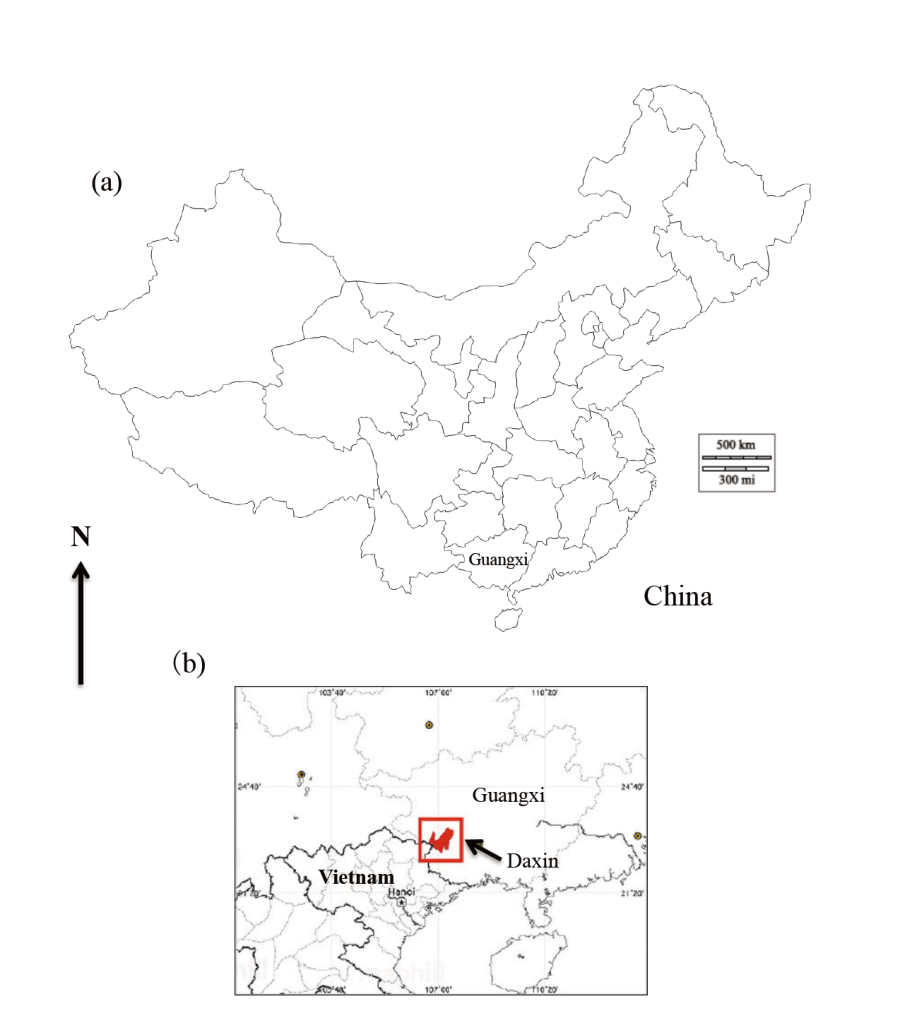
\includegraphics[scale=1]{Figures/Fig21.pdf}
  \caption[Locations of study sites]{Locations of study sites. (a) The Guangxi Zhuang Autonomous Region,
China, (b) the Daxin County (maps from www.maphill.com).}
\end{figure}

\begin{figure}
  \centering
    \label{fig:Fig22}
  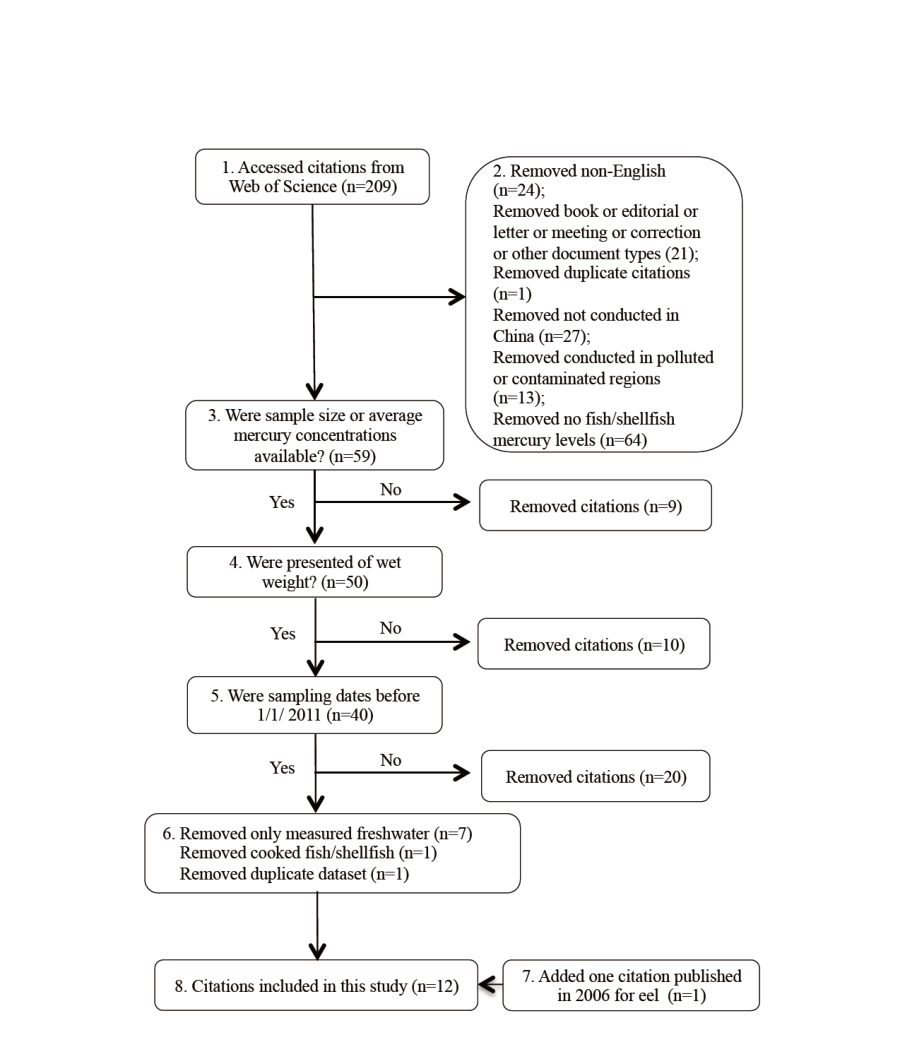
\includegraphics[scale=1]{Figures/Fig22.pdf}
  \caption[Flow chart of the literature search for the total mercury concentrations of
fish/shellfish]{Flow chart of the literature search for the total mercury concentrations of
fish/shellfish.}
\end{figure}

\begin{figure}
  \centering
    \label{fig:Fig23}
  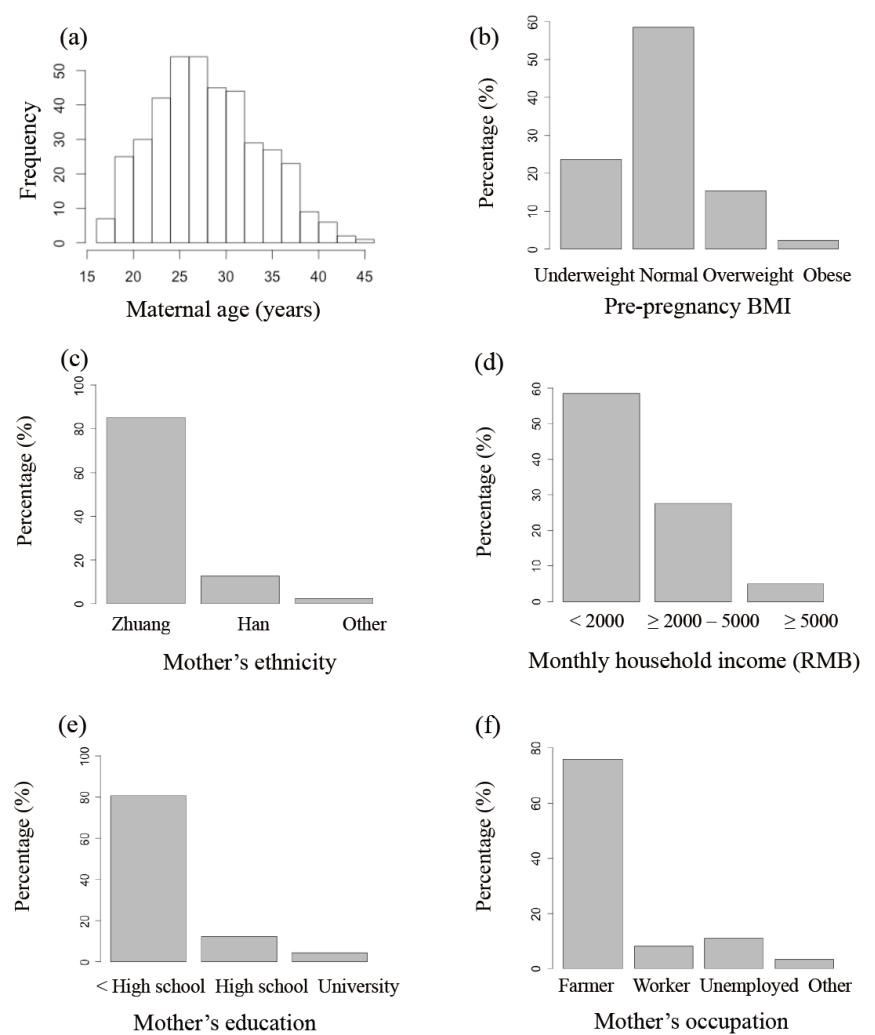
\includegraphics[scale=1]{Figures/Fig23.pdf}
  \caption[Distributions of (a) maternal age, (b) pre-pregnancy body mass index,
(c) mother's ethnicity, (d) monthly household income, (e) mother's education, and (d)
mother's occupation]{Distributions of (a) maternal age, (b) pre-pregnancy body mass index (BMI),
(c) mother's ethnicity, (d) monthly household income, (e) mother's education, and (d)
mother's occupation.}
\end{figure}

\begin{figure}
  \centering
    \label{fig:Fig24}
  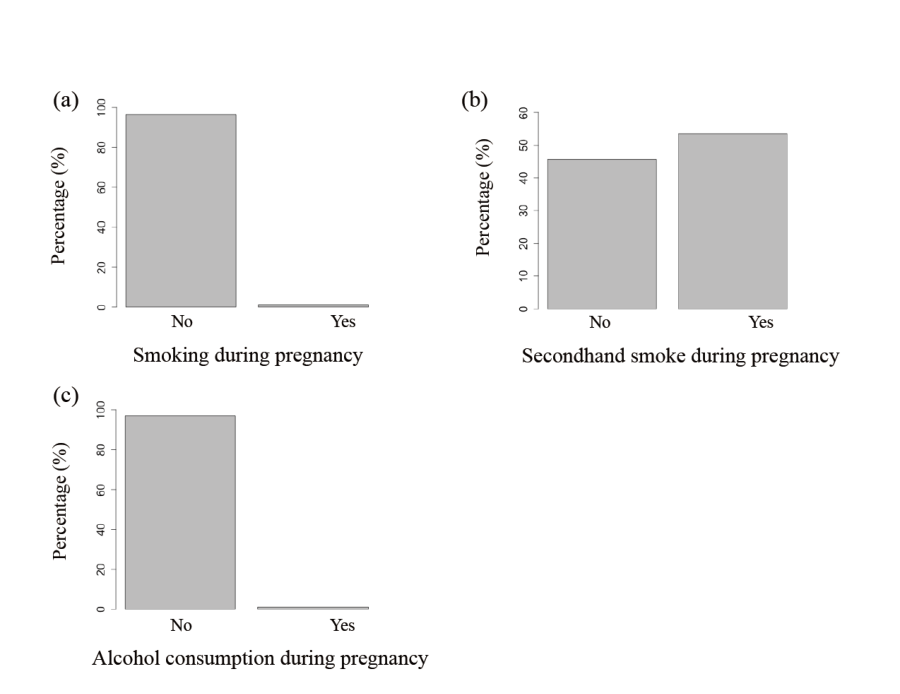
\includegraphics[scale=1]{Figures/Fig24.pdf}
  \caption[Distributions of (a) smoking during pregnancy, (b) secondhand smoke during
pregnancy, and (c) alcohol during pregnancy]{Distributions of (a) smoking during pregnancy, (b) secondhand smoke during pregnancy, and (c) alcohol during pregnancy.}
\end{figure}

\begin{figure}
  \centering
    \label{fig:Fig25}
  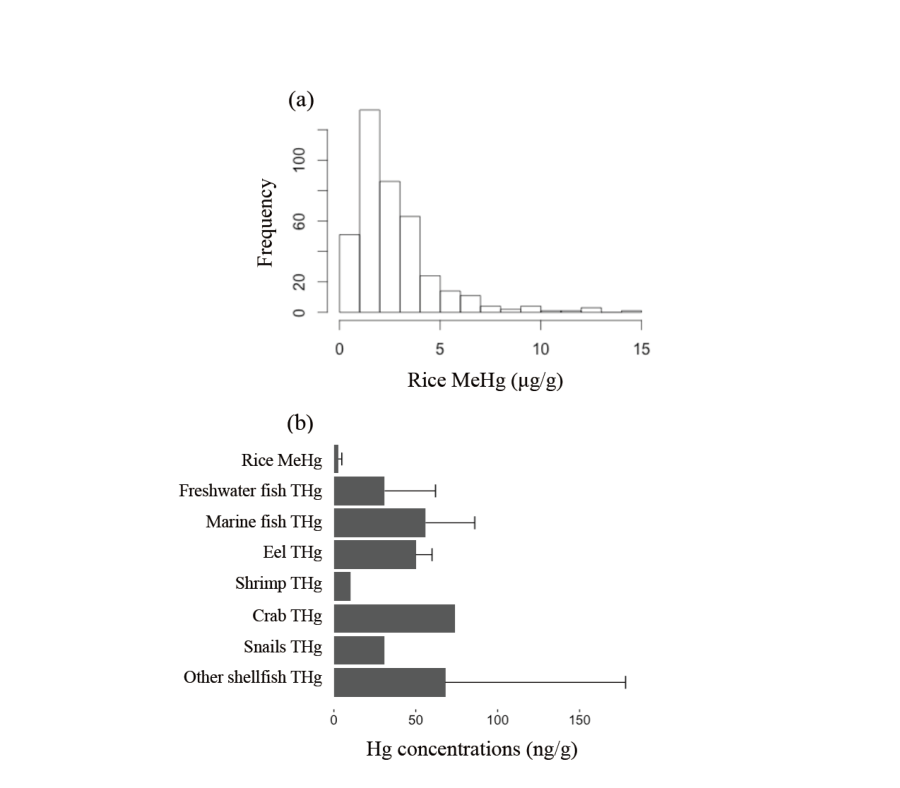
\includegraphics[scale=1]{Figures/Fig25.pdf}
  \caption[Distributions of rice and fish/shellfish mercury levels]{Distributions of rice and fish/shellfish mercury levels. (a) Histogram of the rice methylmercury (MeHg) concentrations, (b) bar chart of the rice MeHg concentrations and total mercury (THg) concentrations for each fish/shellfish variety. For marine fish and other shellfish, the average and SD were weighted based on sample size; for eel, the average and SD was provided by original study; for shrimp, crab, and
snails, the SD was not provided by original studies.}
\end{figure}

\begin{figure}
  \centering
    \label{fig:Fig26}
  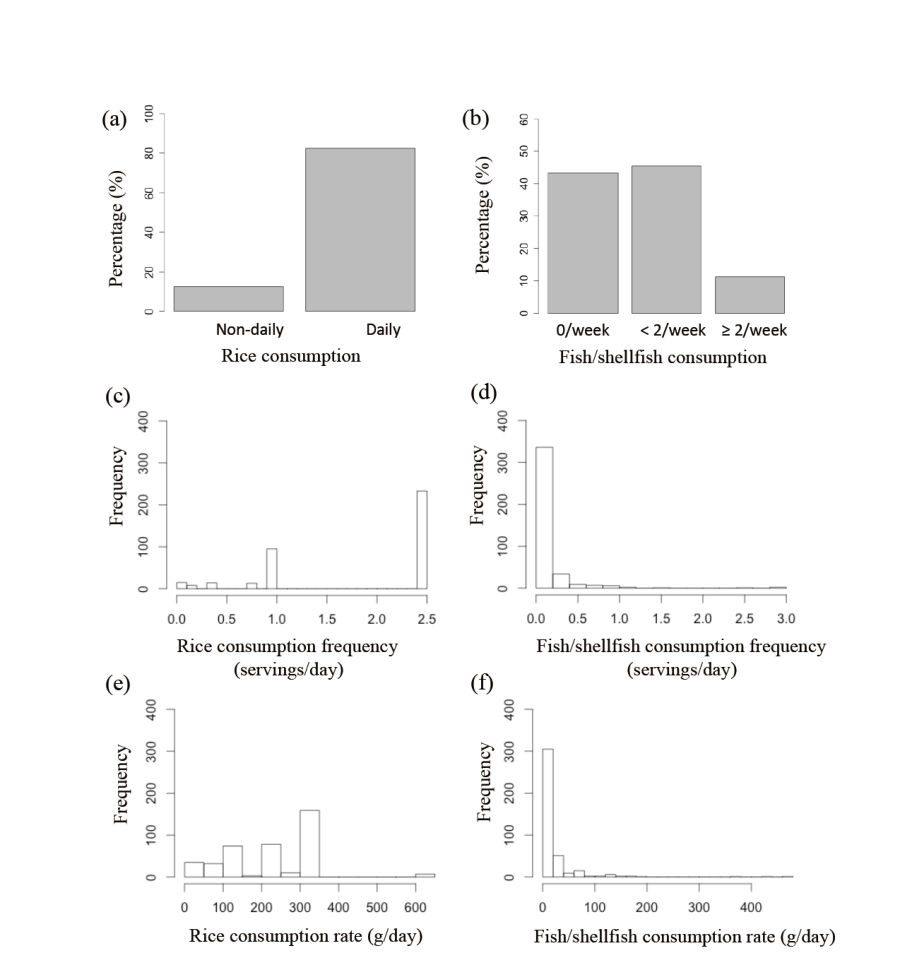
\includegraphics[scale=1]{Figures/Fig26.pdf}
  \caption[Distributions of rice consumption and fish/shellfish consumption]{Distributions of rice consumption and fish/shellfish consumption. (a) Rice consumption (non-daily vs. daily), (b) fish/shellfish consumption (rarely or never, < twice/week, ${\ge}$ twice/week), (c) rice consumption frequency (servings/day), (d) fish/shellfish consumption frequency (servings/day), (e) rice ingestion rate (g/day), and (f) fish/shellfish ingestion rate (g/day).}
\end{figure}

\begin{figure}
  \centering
    \label{fig:Fig27}
  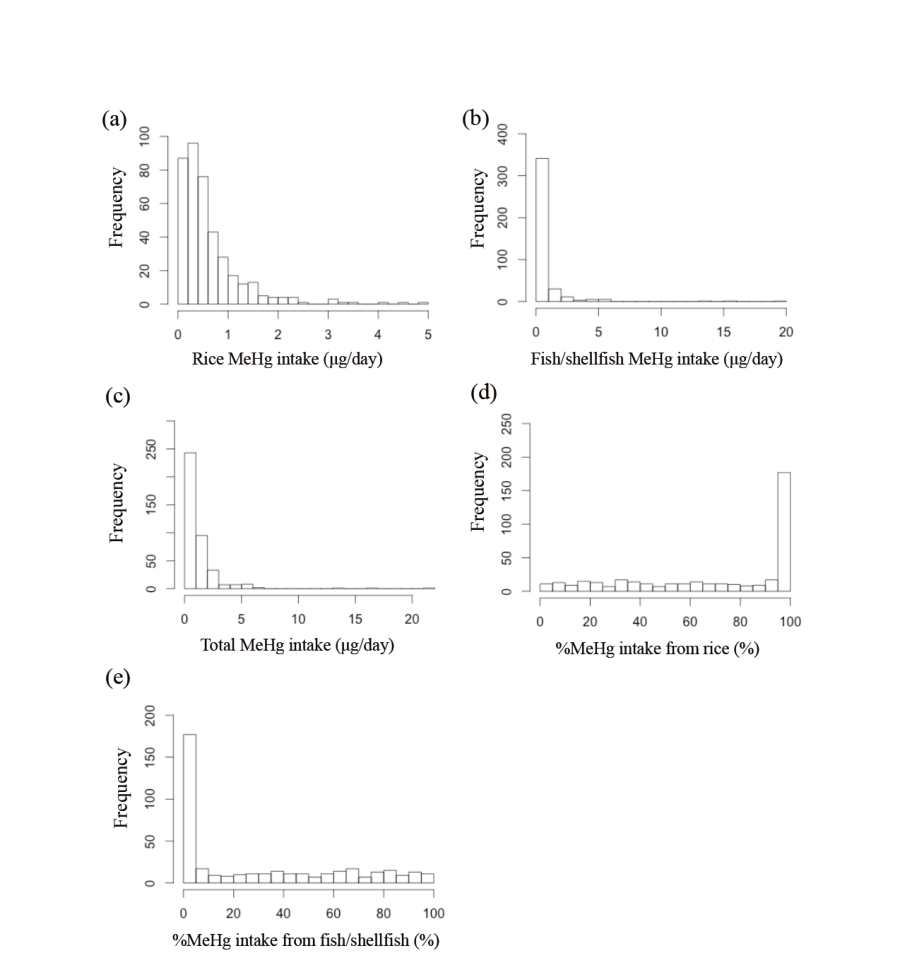
\includegraphics[scale=1]{Figures/Fig27.pdf}
  \caption[Distributions of rice and fish/shellfish methylmercury intake]{Distributions of rice and fish/shellfish methylmercury (MeHg) intake. (a) Rice MeHg intake, (b) fish/shellfish MeHg intake, (c) total MeHg intake through rice and fish/shellfish ingestion, (d) percentage of total MeHg intake from rice consumption, and (e) percentage of total MeHg intake from fish/shellfish consumption.}
\end{figure}

\begin{figure}
  \centering
    \label{fig:Fig28}
  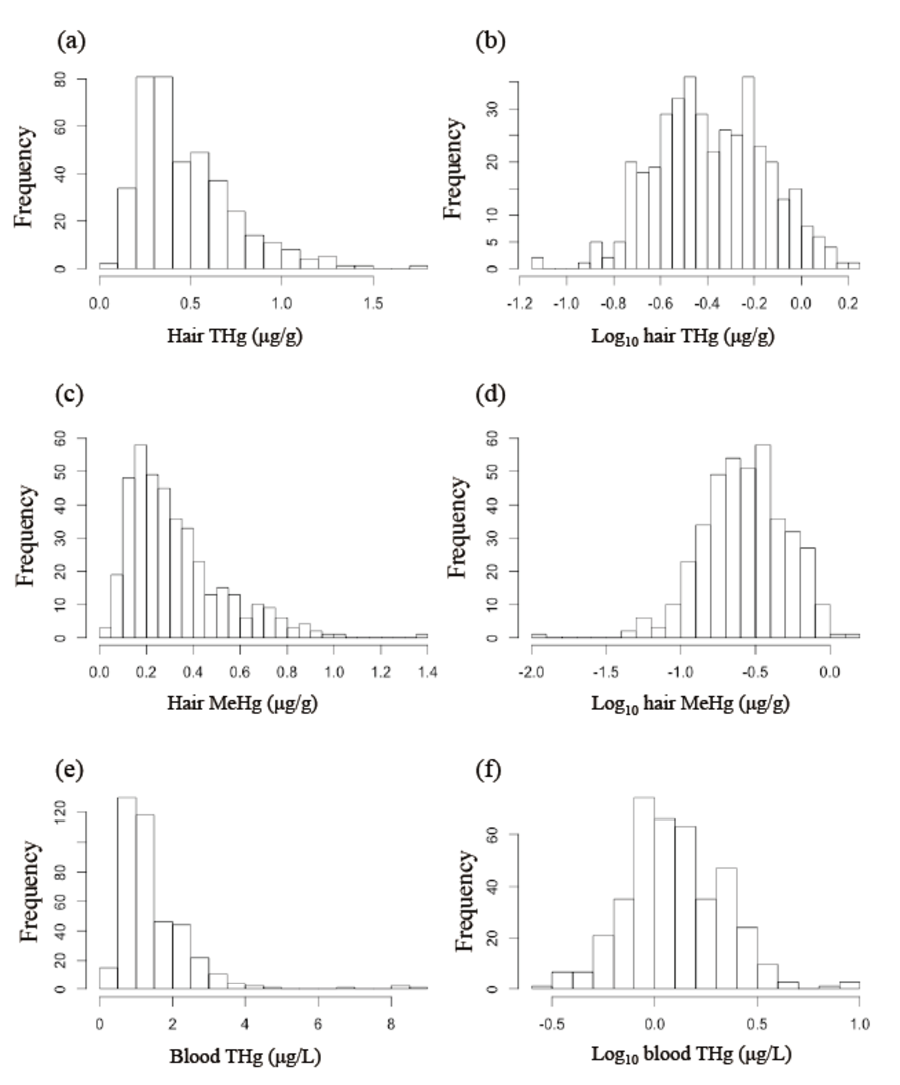
\includegraphics[scale=1]{Figures/Fig28.pdf}
  \caption[Histograms of (a) hair total mercury, (b) $\log_{10}$ hair total mercury, (c) hair methylmercury, (d) $\log_{10}$ hair methylmercury, (e) blood total mercury, and (f) $\log_{10}$ blood total mercury]{Histograms of (a) hair total mercury (THg), (b) $\log_{10}$ hair THg, (c) hair methylmercury (MeHg), (d) $\log_{10}$ hair MeHg, (e) blood THg, and (f) $\log_{10}$ blood THg}
\end{figure}

\begin{figure}
  \centering
    \label{fig:Fig29}
  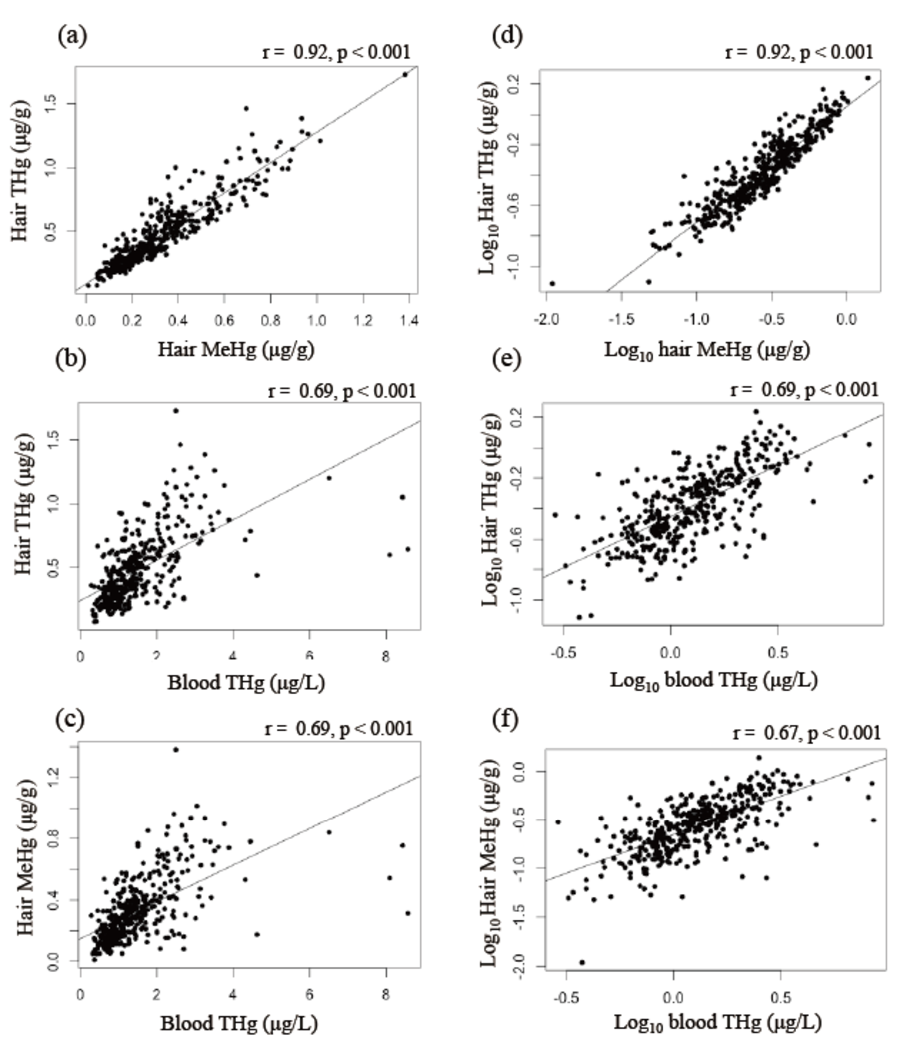
\includegraphics[scale=1]{Figures/Fig29.pdf}
  \caption[Bivariate analyses of hair total mercury, hair methylmercury, and blood total mercury.]{Bivariate analyses of hair total mercury (THg), hair methylmercury (MeHg), and blood THg. Spearman's correlation test for (a) hair MeHg vs. hair THg (r=0.92, p<0.001, n=398), (b) blood THg vs. hair THg (r=0.69, p<0.001, n=397), (c) blood THg vs. hair MeHg (r=0.69, p<0.001, n=397). Pearson's correlations test for (d) $\log_{10}$ hair MeHg vs. $\log_{10}$ hair MeHg (r=0.92, p<0.001, n=398), (e) $\log_{10}$ blood THg vs. $\log_{10}$ hair THg (r=0.69, p<0.001, n=397), (f) $\log_{10}$ blood THg vs. $\log_{10}$ hair MeHg (r=0.67, p<0.001, n=397).}
\end{figure}

\begin{figure}
  \centering
    \label{fig:Fig210}
  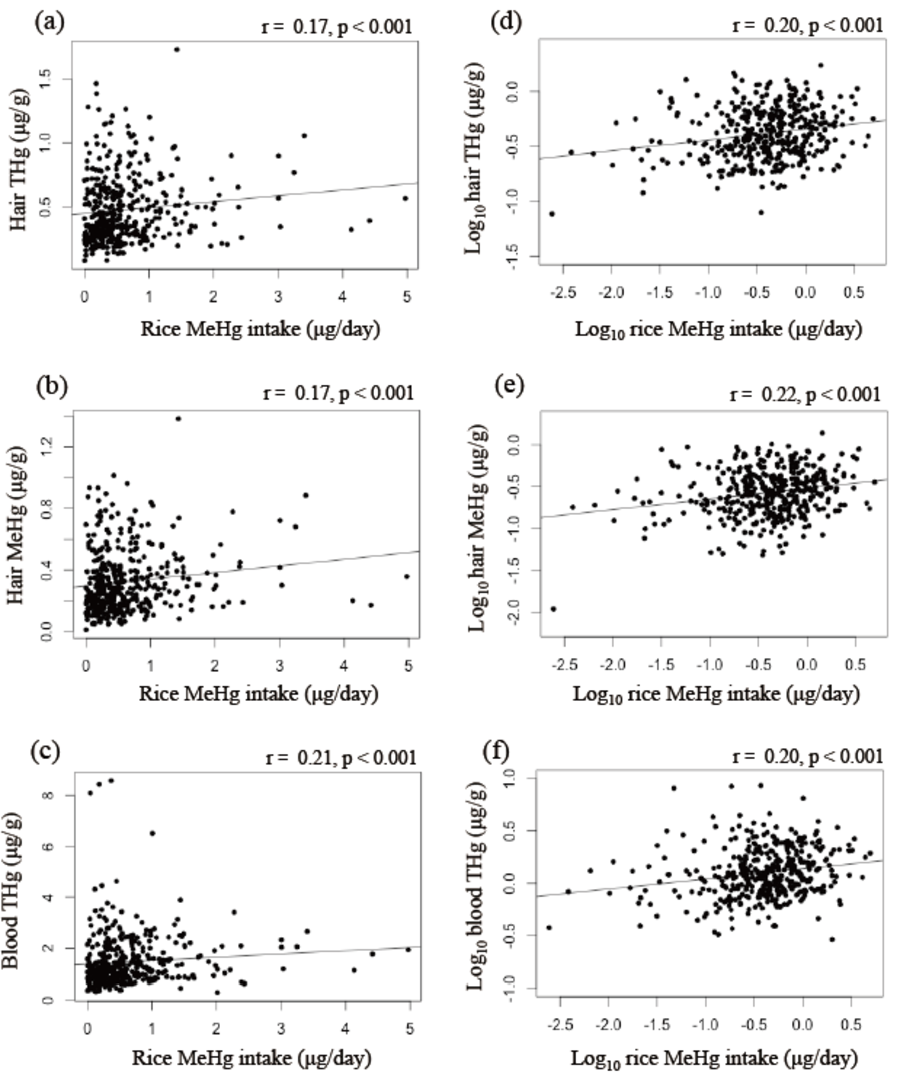
\includegraphics[scale=1]{Figures/Fig210.pdf}
  \caption[Bivariate analyses of rice methylmercury intake and mercury biomarkers]{Bivariate analyses of rice methylmercury (MeHg) intake and mercury biomarkers. Spearman's correlation test for (a) rice MeHg intake versus hair total mercury (THg) (r=0.17, p<0.001), (b) rice MeHg intake versus hair MeHg (r=0.17, p<0.001), (c) rice MeHg intake versus blood THg (r=0.21, p<0.001). Pearson's correlation test for (d) $\log_{10}$ rice MeHg intake versus $\log_{10}$ hair THg (r=0.20, p<0.001), (e) $\log_{10}$ rice MeHg intake versus $\log_{10}$ hair MeHg (r=0.22, p<0.001), and (f) $\log_{10}$ rice MeHg intake versus $\log_{10}$ blood THg (r=0.20, p<0.001) (n=397-398).}
\end{figure}

\begin{figure}
  \centering
    \label{fig:Fig211}
  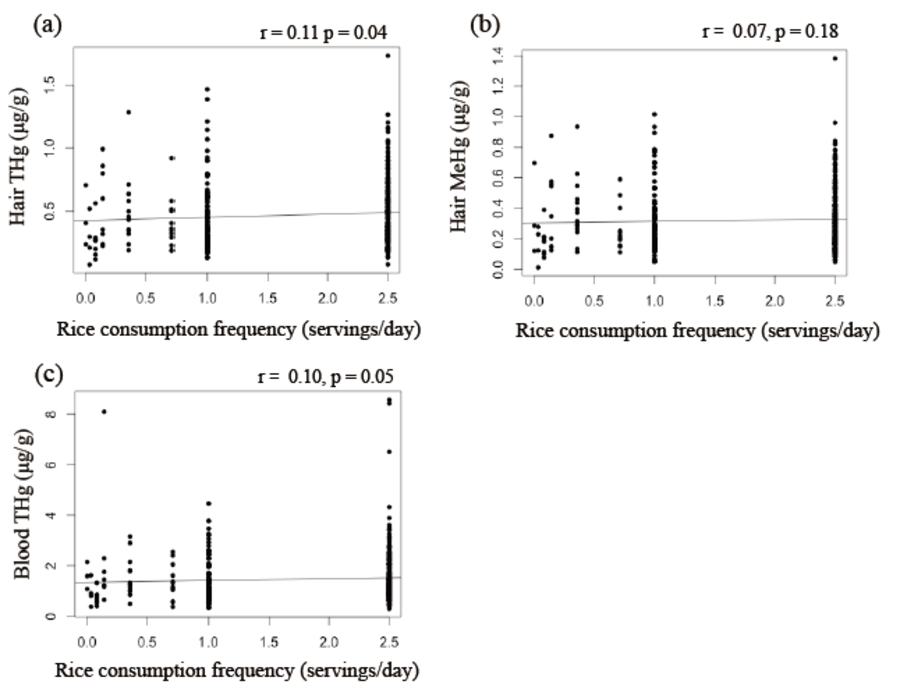
\includegraphics[scale=1]{Figures/Fig211.pdf}
  \caption[Bivariate analyses of rice consumption frequency and mercury biomarkers]{Bivariate analyses of rice consumption frequency and mercury biomarkers. (a) Rice consumption frequency versus hair total mercury (THg) (r=0.11, p=0.04), (b) rice consumption frequency versus hair methylmercury (MeHg) (r=0.07, p=0.18), (c) rice consumption frequency versus blood THg (r=0.10, p=0.05) (Spearman's correlation test for all, n=377-378).}
\end{figure}

\begin{figure}
  \centering
    \label{fig:Fig212}
  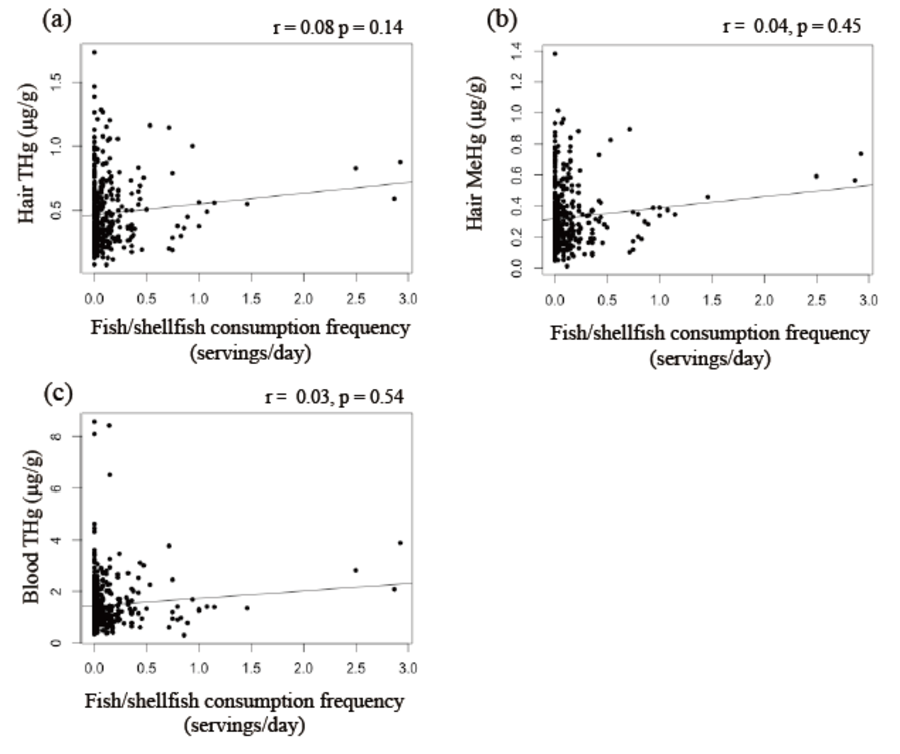
\includegraphics[scale=1]{Figures/Fig212.pdf}
  \caption[Bivariate analyses of fish/shellfish consumption frequency and mercury biomarkers]{Bivariate analyses of fish/shellfish consumption frequency and mercury biomarkers. (a) Fish/shellfish consumption frequency versus hair total mercury (THg) (r=0.08, p=0.14), (b) fish/shellfish consumption frequency versus hair methylmercury (MeHg) (r=0.04, p=0.45), (c) fish/shellfish consumption frequency versus blood THg (r=0.03, p=0.54) (Spearman's correlation test for all, n=397-398).}
\end{figure}

\begin{figure}
  \centering
    \label{fig:Fig213}
  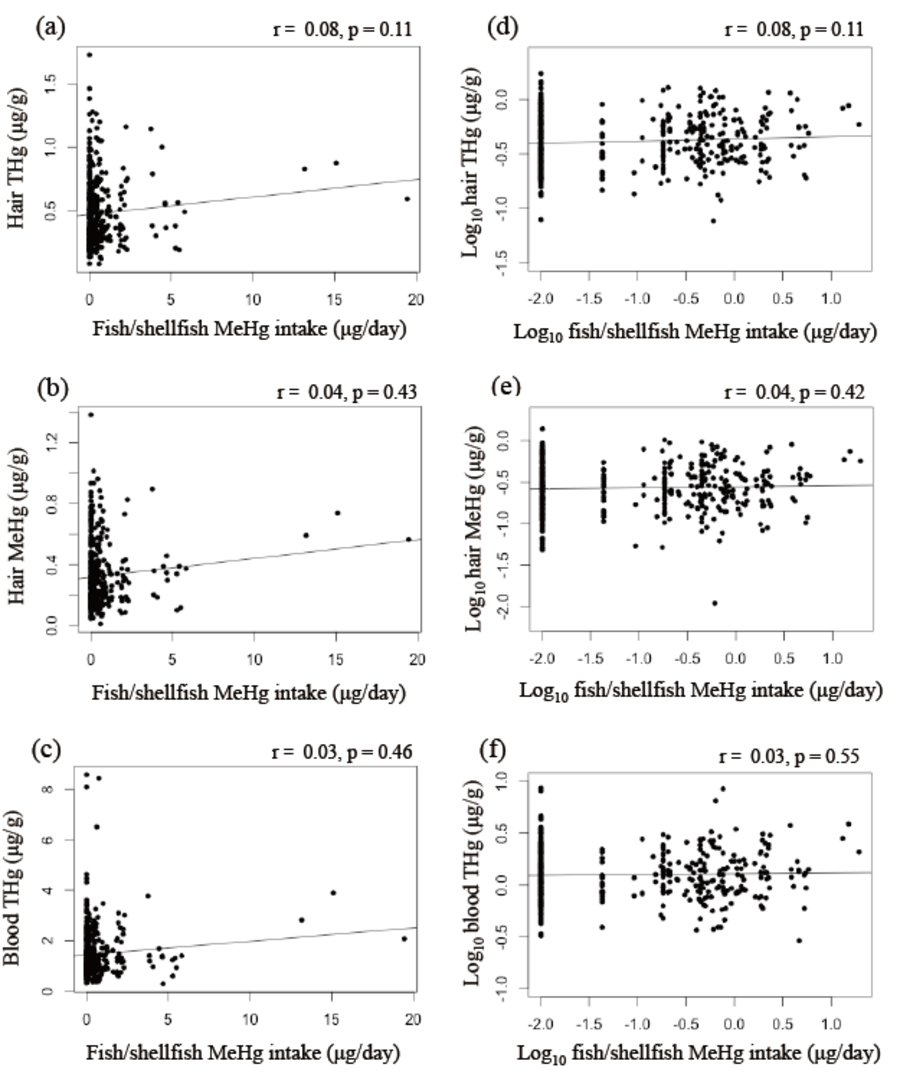
\includegraphics[scale=1]{Figures/Fig213.pdf}
  \caption[Bivariate analyses of fish/shellfish methylmercury intake and mercury biomarkers]{Bivariate analyses of fish/shellfish methylmercury (MeHg) intake and mercury biomarkers. Spearman's correlation test for (a) fish/shellfish MeHg intake versus hair total mercury (THg) (r=0.08, p=0.11), (b) fish/shellfish MeHg intake versus hair MeHg (r=0.04, p=0.45), (c) fish/shellfish MeHg intake versus blood THg (r=0.03, p=0.46). Pearson's correlation test for (d) $\log_{10}$ fish/shellfish MeHg intake versus $\log_{10}$ hair THg (r=0.08, p=0.11), (e) $\log_{10}$ fish/shellfish MeHg intake versus $\log_{10}$ hair MeHg (r=0.04, p=0.42), and (f) $\log_{10}$ fish/shellfish MeHg intake versus $\log_{10}$ blood THg (r=0.03, p=0.55) (n=397-398).}
\end{figure}

\begin{figure}
  \centering
    \label{fig:Fig214}
  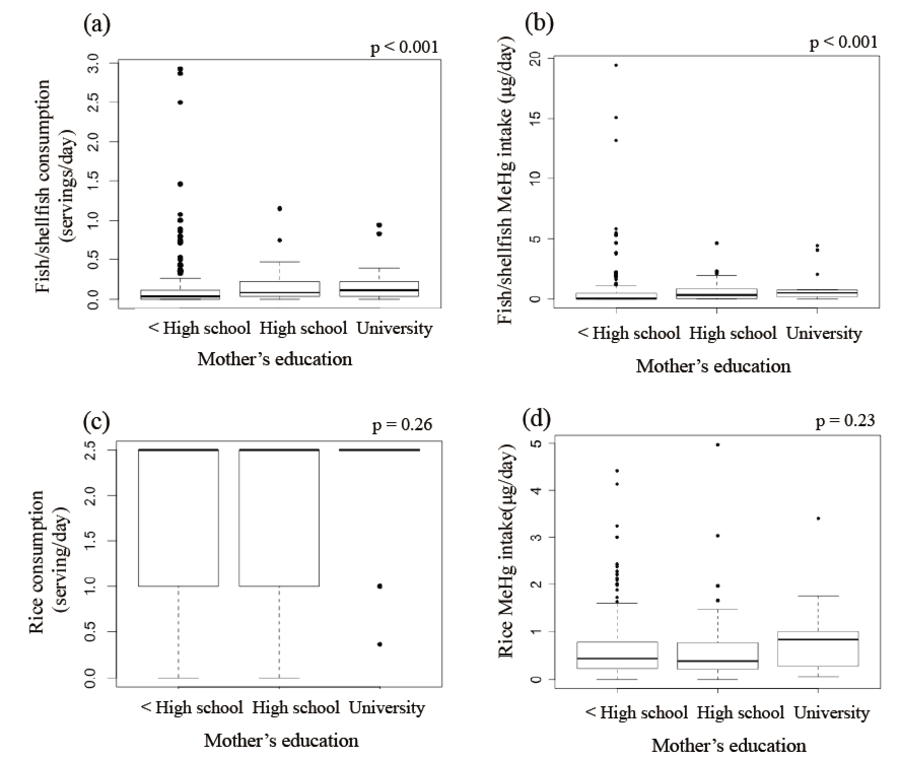
\includegraphics[scale=1]{Figures/Fig214.pdf}
  \caption[Bivariate analyses of mother's education versus fish/shellfish consumption frequency, fish/shellfish methylmercury intake, rice consumption frequency, and rice methylmercury intake]{Bivariate analyses of mother's education versus fish/shellfish consumption frequency, fish/shellfish methylmercury (MeHg) intake, rice consumption frequency, and rice MeHg intake. (a) Education versus fish/shellfish consumption frequency (p<0.001), (b) education versus fish/shellfish MeHg intake (p<0.001)) (c) education versus rice consumption frequency (p=0.26), (d) education versus rice MeHg intake (p=0.23) (Kruskal-Wallis test for all, n=386-388).}
\end{figure}

\begin{figure}
  \centering
    \label{fig:Fig215}
  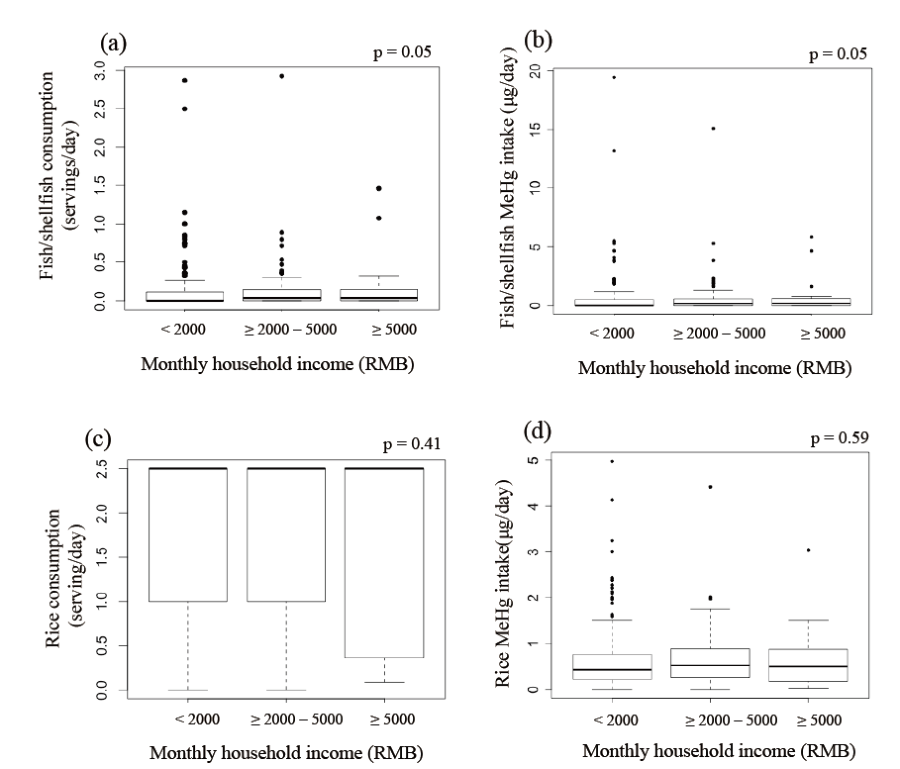
\includegraphics[scale=1]{Figures/Fig215.pdf}
  \caption[Bivariate analyses of monthly household income versus fish/shellfish consumption frequency, fish/shellfish methylmercury intake, rice consumption frequency, and rice methylmercury intake]{Bivariate analyses of monthly household income versus fish/shellfish consumption frequency, fish/shellfish methylmercury (MeHg) intake, rice consumption frequency, and rice MeHg intake. (a) Income versus fish/shellfish consumption frequency (p=0.05), (b) income versus fish/shellfish MeHg intake (p=0.05), (c) income versus rice consumption frequency (p=0.41), (d) income versus rice MeHg intake (p=0.59) (Kruskal-Wallis test for all, n=361-363).}
\end{figure}

\begin{figure}
  \centering
    \label{fig:Fig216}
  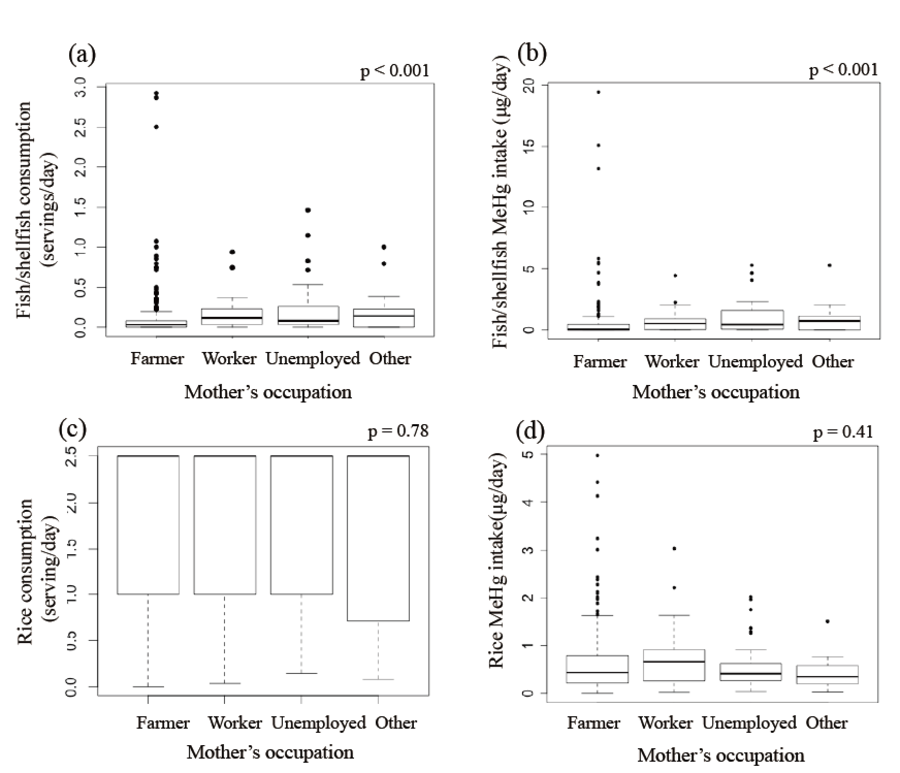
\includegraphics[scale=1]{Figures/Fig216.pdf}
  \caption[Bivariate analyses of mother's occupation versus income versus fish/shellfish consumption frequency, fish/shellfish methylmercury intake, rice consumption frequency, and rice methylmercury intake]{Bivariate analyses of mother's occupation versus income versus fish/shellfish consumption frequency, fish/shellfish methylmercury (MeHg) intake, rice consumption frequency, and rice MeHg intake. (a) Occupation versus fish/shellfish consumption frequency (p<0.001), (b) occupation versus fish/shellfish MeHg intake (p<0.001), (c) occupation versus rice consumption frequency (p=0.78), (d) occupation versus rice MeHg
intake (p=0.41) (Kruskal-Wallis test for all, n=389-391).}
\end{figure}


\begin{figure}
  \centering
    \label{fig:Fig217}
  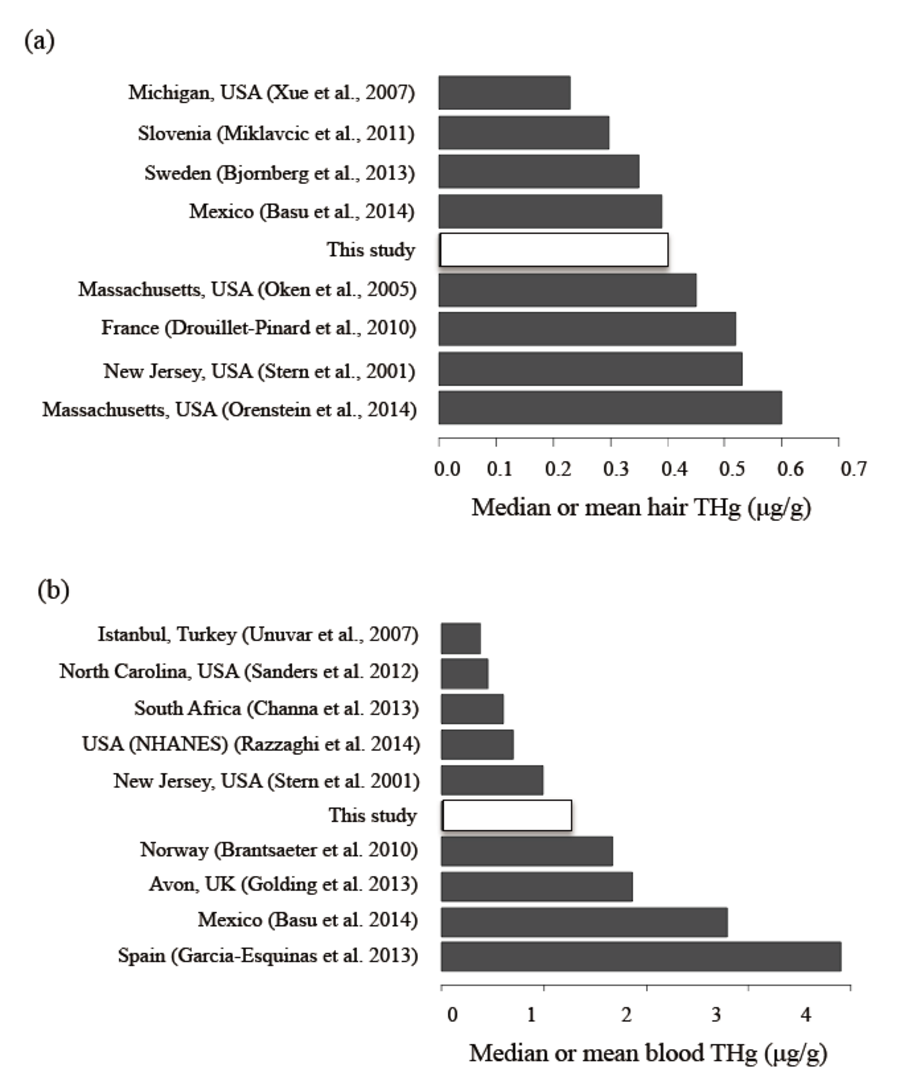
\includegraphics[scale=1]{Figures/Fig217.pdf}
  \caption[Summary of median or mean total mercury concentrations in (a) maternal hair and (b) maternal blood, from studies among pregnant women with low-level mercury exposure]{Summary of median or mean total mercury (THg) concentrations in (a) maternal hair and (b) maternal blood, from studies among pregnant women with low-level mercury exposure (see Table 2.7 for more detail).}
\end{figure}























\chapter{Prenatal Methylmercury Exposure and Neonatal Anthropometry}

\section{Introduction}

Methylmercury (MeHg) is a potent neurotoxin, and it poses a significant risk to human health \citep{mergler2007methylmercury}; National Research Council, 2000). A developing fetus is particularly susceptible to the adverse effects caused by MeHg exposure, as MeHg can readily cross the placenta and pass through the blood brain barrier \citep{clarkson2006toxicology}. A recent review on the human health effects of MeHg exposure indicated that some studies showed that maternal exposure to low-level MeHg during pregnancy had adverse effects on fetal growth, such as birth weight \citep{karagas2012evidence}.

Impaired fetal growth is associated with a number of adverse health effects throughout the lifespan, including neonatal mortality and morbidity \citep{bernstein2000morbidity} and some chronic diseases later in life \citep{barker2006adult,kajantie2005size}. Weight and length at birth are important indicators of developing health conditions. For example, infants born small-for-gestational age (SGA, birth weight for gestational age < 10th percentile) were observed to be at greater risk for developing hypothermia and hypoglycemia during childhood \citep{doctor2001perinatal}. Children born with low birth weight (birth weight < - 2 SD) showed a transition toward adiposity and insulin resistance when they were 2 to 4 years old \citep{ibanez2006early}. Variations in birth length have been associated with the risk of perinatal and postnatal mortality \cite{melve2000infants,cheung2002size}. Restricted brain growth due to severe intrauterine growth restriction was observed to affect the development of cognitive abilities after birth \cite{frisk2002importance}. Additionally, inhibited fetal growth has shown to be associated with some chronic diseases in adulthood, such as high systolic blood pressure,
cardiovascular disease, and type 2 diabetes \citep{barker2006adult}.

The ponderal index (\(\text{birth weight} / \text{birth length}^{3}\)) is used to identify disproportionate fetal growth. The ponderal index was found to be associated with the risk of perinatal and postnatal mortality \citep{cheung2002size}. High ponderal index (${\ge}$ 3.17 g/cm$^{3}$ ${\times}$ 100) was observed to be positively associated with obesity in a cohort of elementary school children in first grade (mean age was 6.1 \({\pm}\) 0.3 years) \cite{loaiza2011birth}. Low ponderal index has been associated with an increased risk of coronary heart disease among adult men \citep{eriksson2001size} or insulin resistance by 10 years of age \citep{larnkjaer2011thin}.

Risk factors for fetal growth are numerous, including maternal demographic or socioeconomic characteristics, health status and nutritional status during pregnancy, and environmental exposures (World Health Organization, 2004b; \cite{de2004risk,triche2007environmental,barger2010maternal}. Some epidemiological studies have shown that prenatal exposure to specific environmental toxins may result in adverse birth outcomes. For example, a Baltimore study observed weak negative associations between cord serum levels of perfluorooctane sulfonate and perfluorooctanoate and birth weight, head circumference, and ponderal index \citep{apelberg2007cord}. A Chinese study reported that prenatal exposure to high-level manganese (${\ge}$ 5.0 ${\mu}$g/L in cord blood) was associated with a high prevalence of high ponderal index (${\ge}$3.17 g/cm$^{3}$ \({\times}\) 100) \citep{yu2013elevated}.

The associations between prenatal exposure to low-level MeHg during pregnancy and neonatal outcomes (such as birth weight, birth length, head circumference, and ponderal index) have been evaluated in some epidemiological studies, yet the results are varied. Some studies have found significant associations between low-level prenatal mercury (Hg) exposure and birth weight, birth length, or ponderal index \citep{wells2016cord,ramon2010fish,gundacker2010perinatal,lee2010interaction,ou2015low}. For example, a Spanish study (n = 554) observed that birth weight decreased with increasing cord blood total mercury (THg) [geometric mean (GM) = 9.4 ${\mu}$g/L] after adjusting for potential variables (fish intake, vegetable intake, energy intake, maternal age, pre-pregnancy weight, gestational weight gain, parity, and smoking status) \citep{ramon2010fish}. A study in South Korea (n = 417) observed significant inverse relationships between maternal blood Hg (GM = 3.3 ${\mu}$g/L) and cord blood Hg (GM = 5.53 ${\mu}$g/L) concentrations and birth weight in both unadjusted and adjusted models [covariates: gestational age, pre-pregnancy body mass index (BMI), maternal age, maternal education level, infant sex, parity, and weight gain during pregnancy] \citep{lee2010interaction}. A study conducted in north China (n = 50) observed significant negative associations
between maternal blood THg (GM = 2.29 ${\mu}$g/L) and birth weight and length in adjusted models (covariates: residential location, maternal age, gestational length, parity, infant sex, maternal after-delivery weight or height, and paternal and parental weight or height) \citep{ou2015low}. An Austria study (n = 53) showed that maternal hair THg (median = 0.184 ${\mu}$g/g) was significantly positively correlated with birth length in bivariate analysis \citep{gundacker2010perinatal}. Finally, a study in Baltimore (n = 271) observed significantly inverse associations between cord blood MeHg (GM = 0.94 ${\mu}$g/L) and ponderal index in both unadjusted and adjusted models [covariates: infant sex, gestational age, maternal age, primiparity, pre-pregnancy BMI, maternal race, maternal smoking, maternal pregestational and gestational hypertension, maternal pregestational and gestational diabetes, cord serum selenium (Se), cord serum omega 3 - highly unsaturated fatty acids (n-3 HUFAs), and cord blood inorganic Hg (IHg)] \citep{wells2016cord}.

However, no significant associations between prenatal low-level MeHg exposure and neonatal outcomes (birth weight, birth length, and head circumference) were observed in a few studies (Daniels et al., 2007; Ding et al., 2013; B.-Q. Guo et al., 2013). For example, a British study (n = 7375) reported that the cord tissue THg (median = 0.01 median = 0.184 ${\mu}$g/g wet weight) was not related to gestational age or birth weight in adjusted models (gestational age, infant sex, birth order, maternal fish consumption, age, education, other dental history variables, prenatal smoking and alcohol use) (Daniels et al., 2007). A study conducted in rural northern China (n = 258) reported no significant associations between maternal blood THg (GM = 0.83 ${\mu}$g/L) or cord blood THg (GM = 1.46 ${\mu}$g/L) levels and birth weight, length, and head circumference in adjusted models (gestational age, parity, infant sex, pre-pregnancy BMI, weight gain during pregnancy, maternal age, household monthly income, and smoking during pregnancy) (Ding et al., 2013). There are a number of factors that likely contributed to differences in previous findings, including differences in biomarkers, covariates, and adjustment for rice and/or fish/shellfish consumption.

In this chapter, we evaluated the associations between prenatal MeHg exposure and neonatal anthropometrics, including birth weight, birth length, head circumference, and ponderal index, in a population living in rural China, where rice ingestion was an important MeHg exposure pathway. Meanwhile, we investigated whether the MeHg exposure impacts would change after adjusting for rice consumption, fish/shellfish consumption, and maternal serum Se.

\section{Methods}

\subsection{Recruitment and data collection}

The study site was located in Daxin County, Guangxi Zhuang Autonomous Region. Briefly, between May 2013 and March 2014, pregnant women were recruited at parturition at the local Maternal and Child Health Hospital. Eligible mothers were those with a singleton pregnancy, in good general health, who had resided in Daxin County during the three previous months and planned to remain for the next year. Written informed consent was obtained from each mother prior to enrollment in this study.
After enrollment, about 50 strands of maternal hair from the occipital region were collected by trained nurses and stored at room temperature in a plastic bag. A non-fasting maternal blood sample was collected by venipuncture (6 ml) into two vials, including one with lithium heparin anticoagulant, and a second vial for separation of serum by centrifugation (3600 rpm, 10 min). Whole blood and serum were stored frozen at -26 \({^\circ}\)C, and then at -80 \({^\circ}\)C.

During their hospital stay, the mothers completed a questionnaire, which included questions about maternal demographic and socioeconomic status (maternal age, height, pre-pregnancy weight, education level, occupation, and monthly household income), maternal characteristics (smoking status and alcohol consumption during pregnancy), and pregnancy history (primipara). Mothers also filled out a modified semi-quantitative food frequency questionnaire (FFQ) \cite{cheng2009assessment}, corresponding to their diet during the third trimester. Food categories included rice and seven commonly consumed
varieties of fish/shellfish (i.e. freshwater fish, marine fish, shrimp, eel, crab, snail and other shellfish). For each food item, the FFQ provided eight options, raging from ``rarely or never'' to ``${\ge}$ twice/week''. With regard to the rice ingestion, mothers also reported quantity per serving by selecting one of three bowls from a picture or actual bowls. Then, rice ingestion rate (g/day) and fish/shellfish consumption frequency (rarely or never, < twice/week, and ${\ge}$ twice/week) were calculated based on the FFQ. For rice ingestion rate (g/day), missing observations (8.5\%) were imputed based on the multivariate normal distribution \cite{schafer1997analysis}.

Information on the current delivery and neonatal outcomes was collected shortly after birth. Birth weight (grams), birth length (cm), head circumference (cm), offspring gender, delivery method, gestational age at delivery, and gestational weight gain were based on electronic medical records.

Percentiles and z-scores for birth weight, birth length, and head circumference according to gestational age and offspring gender were calculated using international newborn standards which were published by the International Fetal and Newborn Growth Consortium for the 21st Century (INTERGROWTH-21$^{st}$) Project \cite{villar2014international}. The INTERGROWTH-21$^{st}$ is a multicenter, multiethnic, population-based project, which was conducted in eight countries (Brazil, China, India, Italy, Kenya, Oman, UK, and USA) \citep{villar2013objectives}. Also, the INTERGROWTH-21$^{st}$ project selected healthy cohorts with no obvious risk factors for intrauterine growth restriction \citep{villar2013objectives}.

SGA by weight (or length or head circumference) was defined as < 10th percentile of birth weight (or birth length or head circumference) for gestational age and gender; large-for-gestational age (LGA) by weight (or length or head circumference) was defined as > 90th percentile of birth weight (or birth length or head circumference) for gestational age and gender; otherwise, newborns were classified as appropriate-for-gestational age (AGA) by weight (or length or head circumference). Ponderal index (g/cm$^{3}$ \({\times}\) 100) was calculated as the ratio of birth weight (grams) to birth length (cm) cubed, multiplied by 100. Protocols were reviewed and approved by the Institutional Review Boards at the University of South Carolina (USA) and Xin Hua Hospital (China).

\subsection{Laboratory analysis and quality assurance/quality control (QA/QC)}

We measured THg and MeHg concentrations in maternal hair, THg concentrations in maternal blood, and Se concentrations in maternal serum. Briefly, maternal hair samples corresponding to the third trimester (34 mm) were analyzed. Before analysis, exogenous Hg was removed by washing hair samples in 0.1\% (v/v) 2- mercaptoethanol. Then, samples were triple-rinsed in double-distilled water (DDI-H2O) and air-dried in a biosafety cabinet (Baker Company, Sanford, USA). After washing, hair
THg was measured without digestion by atomic absorption spectrometry (AAS) using a Lumex Model RA-915+/pyro-915+ (St. Petersburg, Russia) following EPA Method 7473 (U.S. Environmental Protection Agency (USEPA), 2007). Hair MeHg was extracted in 2 ml of 25\% (w/v) sodium hydroxide (NaOH) : DDI-H2O for 3 hours at 75 \({^\circ}\)C, then diluted with boiling DDI-H2O. The extracts of hair MeHg were analyzed using a gas chromatography-cold vapor atomic fluorescence spectrometry (Brooks Rand Model III, Seattle, WA, USA) following EPA Method 1630 (U.S. Environmental Protection Agency (USEPA), 2001a).

Blood THg was measured using a DMA-80 (Milestone, Inc., Shelton, CT, USA) following EPA Method 7473 (U.S. Environmental Protection Agency (USEPA), 2007). Serum Se was analyzed by inductively coupled plasma-mass spectrometry (Agilent 7500CE, USA) following EPA Method 3050B (U.S. Environmental Protection Agency (USEPA), 1996).

The QA/QC for maternal biomarkers analyses were ensured by the use of standard reference materials (SRM), matrix spike recoveries, and relative percent difference (RPD) for analysis of replicates, which was summarized in Table 3.1. In addition, the limits of detection were: hair THg (0.0095 ${\mu}$g/g), hair MeHg (0.0001 ${\mu}$g/g), blood THg (0.14 ${\mu}$g/L), and serum Se (1.6 ${\mu}$g/L). All observations were above the limits of detection.

\subsection{Data analysis}

Univariate analysis and bivariate analysis was provided for all variables. We conducted both simple linear regression and multivariable linear regression models to evaluate the associations between maternal Hg biomarkers (maternal hair THg, maternal hair MeHg, and maternal blood THg) and neonatal outcomes (birth weight z score, birth length z score, head circumference z score, and ponderal index). For model analysis, a $\log_{10}$ transformation was applied to right-skewed variables to minimize the disproportional impact of extreme values. These variables were maternal Hg biomarkers, maternal serum Se, and rice ingestion (g/day).

The inclusion of covariates in the multivariable regression models was based on prior studies concerning prenatal MeHg exposure and birth outcomes \citep{choi2008selenium,guo2009formaldehyde,ding2013prenatal,rothenberg2016maternal,wells2016cord}. Covariates used in this study include maternal age (years), pre-pregnancy BMI (underweight, normal, overweight, obese) (World Health Organization, 2004a), maternal
education (< high school, high school, university), gestational age at delivery (weeks), gestational weight gain (kg), offspring gender (female, male), delivery method (cesarean, vaginal), rice ingestion (g/day), fish/shellfish consumption (rarely or never, < twice/week, ${\ge}$ twice/week), and maternal serum Se (${\mu}$g/L), which has been suggested to be a potential protective factor \cite{choi2008selenium,wells2016cord}.

For consistency, the same set of covariates was included in the multivariable regression model for each outcome measure. The models for head circumference z score were additionally adjusted for the delivery mode (Vaginal, Caesarian), in order to be consistent with other studies \cite{guo2009formaldehyde,wells2016cord}. Additionally, the models for birth weight z score, birth length z score, and head circumference z score were
not adjusted for offspring gender and gestational age, because z score was defined based on growth charts for birth size standards by gestational age (weeks) specific for offspring gender \cite{villar2014international} Diagnostics for multivariable linear regression models included investigation of the plots of residuals versus fitted values, investigation of the quantile-quantile plots to check the distribution of the residuals, and Cook?s distance to check for potential outliers. In addition, we used Akaike Information Criterion values to compare models. 

Analyses were performed using SAS 9.4 software (SAS Institute Inc., Cary, NC, USA) and the R-platform. An alpha-level of 0.05 was considered statistically significant.

\section{Results}

\subsection{Maternal and neonatal characteristics}

Over the course of the recruitment period, 1261 mothers gave birth at the local hospital. Among these mothers, 408 provided informed consent. Subsequently, ten mothers were excluded because they did not give birth in the hospital (n = 1), gave birth to twins (n = 1), did not live in Daxin during the previous three months (n = 3), or did not complete data collection (n = 5), leaving a total of 398 study participants. 

In the Daxin cohort, the average maternal age was 28 ${\pm}$ 5.1 years, and most of the mothers had an education level below high school (81\%) and worked as farmers (76\%). 59\% of the participants had a monthly household income below 2000 RMB. Very few of them reported smoking (1.3\%) or drinking alcohol (1.0\%) during pregnancy. 

Among the newborns, 3.5\% (n = 14) were born with low birth weight (< 2,500 g). Based on the percentiles for birth weight, 46 (12\%) and 17 (4.3\%) newborns were classified as SGA (< 10th) and LGA (> 90th), respectively. For percentiles for birth length, there were 12 (3.0\%) with SGA (< 10th) and 151 (38\%) with LGA (> 90th). And, for percentiles for head circumference, there were 163 (50\%) with SGA (< 10th) and 6 (1.5\%) with LGA (> 90th).

Detailed characteristics of these 398 mothers/offspring are summarized in Table 3.2 (see also Figure 2.3, 2.4, 3.1-3.5).

\subsection{Concentrations of Hg and Se in maternal biomarkers}

Detailed results for the maternal Hg biomarkers are described in Chapter 2 (Table 3.2). For the maternal serum Se, the GM concentration was 150 ?g/L (median = 150 ?g/L, range: 66 - 540 ?g/L, Table 3.2). Among 396 pregnant women, 12 mothers (3.0\%) were Se deficient (< 87 ?g/L for non-pregnant women) (Allen, de Benoist, Dary, \& Hurrell, 2006). The distributions of maternal Hg biomarkers and serum Se were shown in Figure 2.8 and 3.2.

\subsection{Bivariate analyses}

\subsubsection {Comparison with other pregnant cohorts with low-level Hg exposure}

Maternal age and Hg biomarkers were found to be positively correlated in some pregnant cohorts \cite{basu2014mercury,bjornberg2003methyl,wells2016cord,xue2007maternal}. These positive correlations reflect the MeHg exposure increasing with age. For example, a Baltimore birth cohort (n = 271) observed that cord blood MeHg increased with increasing maternal age in unadjusted models (beta = 0.019, 95\% CI: -0.0002, 0.037) \citep{wells2016cord}. A Michigan birth cohort (n = 1024) found that higher maternal hair THg levels were significantly associated with older maternal age (${\pm}$ 25 years)\citep{xue2007maternal}. A Mexico birth cohort (n = 348) reported that maternal age was positively associated with blood Hg levels in trimester 2 (beta = 0.015, p < 0.05) and 3 (beta = 0.035, p < 0.05), but not levels in trimester 1 or in cord blood in unadjusted models \citep{basu2014mercury}. A Swedish study (n = 112) found that older mothers had higher maternal hair THg levels, but not cord blood MeHg \citep{bjornberg2003methyl}. The authors from this Swedish study speculated that in their study older women had a higher seafood intake before pregnancy and the seafood consumption decreased during pregnancy \citep{bjornberg2003methyl}.

However, no significant correlation was observed between maternal age and all Hg biomarkers (i.e. hair THg, hair MeHg and blood THg) in the Daxin cohort (Spearman's rho = 0.05 - 0.09, p = 0.08-0.34) (Figure 3.6). Maternal age was borderline positively correlated with blood THg (Spearman's rho = 0.09, p = 0.08). Our findings were similar to a study from Canada \citep{mahaffey1998blood} (n = 288), which did not observe significant relationships between blood THg levels and age in men and women.

\subsubsection{Pre-pregnancy BMI}

Pre-pregnancy BMI is known to be an influencing factor for fetal growth (World Health Organization, 2004b). Several recent studies have observed that pre-pregnancy BMI was positively associated with birth weight \citep{pfrederick2008pre,nohr2008combined}. In a systematic review and meta-analyses, the authors observed that maternal underweight (defined by the original studies) has been shown to increase the risk of preterm birth (< 37 weeks) and low birth weight (< 2,500 g) \citep{han2012maternal}. A Chinese study observed that pre-pregnancy BMI was positively correlated with birth weight, birth length, and ponderal index \citep{yu2013elevated}. As expected, we observed that pre-pregnancy BMI was weakly positively correlated with all neonatal anthropometries (i.e. birth weight, birth length, head circumference, and ponderal index) in this study (Spearman's rho = 0.12-0.21, p < 0.05 for all) (Figures 3.7 and 3.8). 

Additionally, in this study, we observed that pre-pregnancy BMI was negatively correlated with hair THg (Spearman's rho = -0.11, p = 0.03), and borderline with blood THg (Spearman's rho = -0.08, p = 0.09), but not with hair MeHg (Spearman's rho = -0.05, p = 0.28) (Figure 3.9). Our findings were potentially similar to a U.S. study (National Health and Nutrition Examination Survey, 2007-2010) that reported that blood Hg levels for adults were inversely associated with BMI, after controlling for MeHg intake through fish/shellfish ingestion \citep{rothenberg2015influence}.

\subsubsection{Gestational weight gain}

The Institute of Medicine (IOM) published recommendations for weight gain during pregnancy based on pre-pregnancy BMI (Institue of Medicine (IOM), 2009). Excessive gestational weight gain is associated with an increased risk of caesarean delivery and LGA, and inadequate gestational weight gain is associated with an increased risk of SGA \citep{nohr2008combined}. In general, the IOM recommends less weight gain for
increasing pre-pregnancy BMI (Institue of Medicine (IOM), 2009). In this study, we observed that pre-pregnancy BMI was inversely correlated with gestational weight gain (Spearman's rho= -0.23, p < 0.0001) (Figure 3.10), which was consistent with other studies \citep{rode2007association,nohr2008combined,dietz2009low} and IOM recommendations (Institue of Medicine (IOM), 2009). Using the WHO BMI cutoff points for American populations (underweight: less than 18.5 kg/m$^{2}$, normal
weight: 18.5-24.9 kg/m$^{2}$, overweight: 25-29.9 kg/m$^{2}$, obese: 30 and greater kg/m$^{2}$), 209 mothers (53\%) were below the IOM guideline, 105 mothers (26\%) were within the IOM
guidelines, and 83 mothers (21\%) were above the IOM guidelines (Table 3.3).

\subsubsection{Rice and fish/shellfish ingestion}

The mean rice ingestion rate in the Daxin cohort was 231 g /day (median: 210 g/day, range: 0-650 g/day), which was similar to the mean rate in China (214 g/day) (Food and Agriculture Organization of the United Nations (UNFAO), 2016). The statistics test results indicated that there were no significant differences in the rice consumption (g/day) by mother's education level (< high school, high school, university), mother's occupation (farmers, workers, unemployed, other), or household income (< 2000 RMB/month, ${\ge}$ 2000 RMB/month) (Kruskal-Wallis test, p > 0.1 or Wilcoxon- Mann-Whitney test, p > 0.1, Table 2.14, 2.15, and 2.16).

For the fish/shellfish consumption, the mean ingestion rate was 18 g/day (median = 5.6 g/day, range: 0 - 470 g/day), which was lower than the average rate of the general Chinese population (95 g/day) (Food and Agriculture Organization of the United Nations (UNFAO), 2016). The fish/shellfish consumption (g/day) was significantly higher for mothers who completed university (median: < high school = 3.3 g/day; high school = 10 g/day; university = 17 g/day), who were workers or other (median: farmers = 3.3 g/day; workers = 17 g/day; unemployed = 14 g/day; other = 22 g/day), or who had higher monthly household income (RMB/month) (< 2000 = 0 g/day; ${\ge}$ 2000 = 5.6 g/day) (Kruskal-Wallis test or Wilcoxon-Mann-Whitney test, p < 0.05) (Figure 3.11).

Additionally, the rice consumption rate (g/day) was not correlated with fish/shellfish consumption rate (g/day) (Spearman's rho = 0.05, p = 0.27, n=398).

\subsubsection{Hg and Se}

Se is an essential trace metal, which is hypothesized to be a natural antagonist to Hg in mammalian animals. Se is incorporated into selenoproteins which are able to interact with Hg by forming Se-Hg protein compounds \citep{gromer2005human,taylor2009recent}. The Se-Hg interaction may possibly affect MeHg toxicity. For example, an animal study found that the symptoms of neuronal degeneration induced by MeHg in the developing rat cerebrum were prevented by coexposure to Se, which indicated that Se might be an protective factor against MeHg toxicity in mammals \citep{sakamoto2013selenomethionine}. Additionally, a human study observed that among subjects with high Hg exposure, the expression of selenoproteins in serum was increased, however no correlation was observed between serum Hg and Se \citep{chen2006roles}. The authors suggested that the selenoproteins might affect the Hg toxicity by binding more Hg through their highly reactive selenol groups \citep{chen2006roles}. The associations between Se and Hg in pregnant women have received some attention from other researchers. In two Faroe Islands birth cohorts with maternal whale consumption, Se and Hg in cord blood were positively correlated (r=0.35 for the first cohort, n=880 and r=0.29 for the second cohort, n=142) \citep{choi2008selenium}. However, there were no inverse relationships observed between Se and scores of Hg-induced neuropsychological dysfunctions assessments in multivariate regression models \citep{choi2008selenium}. A Baltimore study (n = 271) reported that cord blood MeHg and cord serum Se was not correlated (Spearman's rho = -0.02), and the strength of the relationship between MeHg and birth outcomes (i.e. gestational age, birth weight, birth length, head circumference, and ponderal index) was not affected by the inclusion of Se in multivariable regression models \citep{wells2016cord}. In this study, we observed that hair THg and hair MeHg were not significantly correlated with serum Se (Spearman's rho = 0.06-0.09, p = 0.09-0.20), while blood THg had a weakly positive correlation with serum Se (Spearman's rho = 0.10, p = 0.04) (Figure 3.12).

\subsubsection{Other variables}

Education, occupation, and monthly household income were associated with each other in the Daxin cohort (p < 0.001 for education versus occupation, p = 0.08 for occupation versus monthly household income, p = < 0.01 for education versus monthly household income, Fisher's exact test for all). For example, mothers who were workers mostly had an education level of high school or above and a monthly household income
above 2000 RMB/month.

Additionally, education was marginally correlated with delivery method (Chi-squared test, p = 0.07). Mothers with an education level of high school or above were more likely to deliver their children by cesarean. Among 388 mothers who reported education and delivery method, 37\% of the mothers with a high school degree or above delivered their children by cesarean, whereas 25\% of the mothers with an education level below high school delivered their children by cesarean (Table 3.4).

\subsection{Hg biomarkers and outcome measures}

Unadjusted correlations between Hg biomarkers and outcome measures were investigated. Birth weight z score was weakly inversely correlated with all three Hg biomarkers (Spearman's rho range: |0.10 - 0.11|, p ${\le}$ 0.05 for all), while the ponderal index was weakly inversely correlated only with blood THg (Spearman's rho = -0.11, p=0.03) (Figures 3.13-3.18). However, all other unadjusted correlations between Hg biomarkers and outcome measures (including ponderal index, birth length z score, and head circumference z score) were non-significantly inverse (Spearman's rho range: |<0.01-0.07|, p = 0.15-0.98) (Figures 3.13-3.18).

In adjusted linear models for birth weight z score, birth length z score and head circumference z score, birth weight z score was inversely associated with all three biomarkers, but the trends for log10 hair THg (beta: -0.41, 95\% CI: -0.78, -0.032, p = 0.03) and $\log_{10}$ hair MeHg (beta: -0.31, 95\% CI: -0.63, 0.0013, p = 0.05) were significant, while the trend for $\log_{10}$ blood THg (beta: -0.36, 95\% CI: -0.73, 0.010, p = 0.06) was borderline. For a doubling in $\log_{10}$ hair THg (${\mu}$g/g), the z score for birth weight decreased by 0.12 (95\% CI: -0.23, -0.01); for a doubling in $\log_{10}$ hair MeHg (${\mu}$g/g), the z score for birth weight decreased by 0.09 (95\% CI: -0.19, < 0.01); for a doubling in $\log_{10}$ blood THg (${\mu}$g/L), the z score for birth weight decreased by 0.11 (95\% CI: -0.22, < 0.01). The relationships observed in other adjusted models for Hg biomarkers and outcome measures (birth length z score and head circumference z score) were inverse but nonsignificant (Table 3.5 and Figures 3.19-3.21).

In three adjusted models for ponderal index, ponderal index significantly decreased with increasing $\log_{10}$ blood THg (beta: -0.13, 95\% CI: -0.24, -0.017), but not with other Hg biomarkers (Table 3.5 and Figure 3.22). For a doubling in blood THg (${\mu}$g/L), the ponderal index decreased by 0.04 (g/cm$^{3}$ \({\times}\) 100) (95\% CI: -0.07, < -0.01). Additionally, for all models for ponderal index, we observed two disconnected observations in the plots of residuals versus fitted values (Figure 3.25). These two disconnected observations were the two lowest observations for ponderal index (0.83 and 0.97, g/cm$^{3}$ \({\times}\) 100) (< 10th percentile). After excluding these two disconnected observations, the betas and 95\% CIs for Hg biomarkers and other covariates did not change much (Tables 3.5 and 3.6, and Figure 3.22).

\subsection{Other covariates and outcome measures}

Unadjusted relationships between other covariates [i.e. maternal age (years), prepregnancy BMI (underweight, normal, overweight, obese), gestational weight gain (kg), education (< high school, high school, university), offspring gender, gestational age (years), delivery method (cesarean, vaginal), rice ingestion (g/day), fish/shellfish consumption (rarely or never, < twice/week, ${\ge}$ twice/week), and serum se (${\mu}$g/L)] and outcome measures were investigated. Gestational weight gain was weakly positively
correlated with birth weight z score, birth length z score, head circumference z score (Pearson's rho range: 0.19 - 0.22, p < 0.001 for all), but not with ponderal index (Pearson's rho = 0.06, p = 0.20) (Figure 3.24). Also, gestational age was weakly negatively correlated with head circumference z score (Pearson's rho = -0.14, p = 0.004), and weakly positively correlated with ponderal index (Pearson's rho = 0.10, p = 0.04) (Figure 3.25). Additionally, offspring whose mothers possessed an education level of high school or above were likely to have a larger birth length z score and head circumference z score (One-way ANOVA test, p < 0.05) (Figure 3.26). Offspring delivered by cesarean had a larger head circumference z score than those delivered vaginally (Student's t-test, p < 0.01)(Figure 3.27). No significant relationships were observed between other covariates and outcome measures (Figures 3.28-3.35).

In all 12 adjusted models, gestational weight was still positively associated with birth weight z score (beta = 0.4 for all, p < 0.01), birth length z score (beta = 0.03 for all, p = 0.01), and head circumference z score (beta = 0.04 for all, p < 0.01), but marginally positively associated with ponderal index (beta < 0.01 for all, p = 0.08-0.09). In all three adjusted models for head circumference, delivery method was associated with head circumference z score. We observed that babies born by cesarean had a higher head circumference z score, compared to those delivered vaginally (p < 0.001 for all), and babies whose mothers possessed a high school education level had a marginally higher head circumference than those whose mothers had an education level below high school (beta: 0.26-0.27, p ${\le}$ 0.1 for all). This may be due to the correlations between maternal education and delivery method. After excluding either education or delivery method from
the adjusted models, there were no significant changes for the betas, 95\% CIs, and the models satisfied assumptions, which indicated that they were not confounders quantitatively for the main associations of interest. Additionally, compared to mothers who were underweight, mothers who were overweight had higher birth weight z score (p < 0.01 for all) and z score for head circumference (p < 0.02 for all). No significant associations were observed between other covariates and outcome measures. Detailed
results are summarized in Tables 3.7 - 3.9.

\section{Discussion}

In this study, we included three maternal Hg biomarkers (hair THg, hair MeHg, blood THg) and four birth outcome measures (birth weight, birth length, head circumference, ponderal index), and evaluated each association in unadjusted and adjusted analyses. Our findings indicated that all three Hg biomarkers were inversely related with birth weight z score in adjusted models, the trends were significant for hair THg and hair MeHg, and marginally significant for blood THg. We found similar results for the relationships between all three Hg biomarkers and birth weight z score, birth length z score, and head circumference z score; however, the relationships between Hg biomarkers and the ponderal index were different. In the adjusted model analyses for ponderal index, the trends were non-significant for hair THg and hair MeHg, but significant for blood THg. Additionally, the results showed that the relationships between all Hg biomarkers and neonatal outcomes did not differ greatly between unadjusted and adjusted models.

So far, several studies have evaluated the influences of prenatal low-level MeHg exposure through maternal fish/shellfish ingestion on neonatal anthropometrics, and have shown varied results \citep{daniels2007maternal,ramon2010fish,gundacker2010perinatal,lee2010interaction,ding2013prenatal,ou2015low,wells2016cord}
\citep{daniels2007maternal,ramon2010fish,gundacker2010perinatal,lee2010interaction,ding2013prenatal,ou2015low,wells2016cord}. Similar to the previous studies reporting inverse relationships between birth weight and some Hg biomarkers in fish-eating populations, such as cord blood THg \citep{ramon2010fish,lee2010interaction} or maternal blood THg \citep{lee2010interaction,ou2015low}, we observed that birth weight z score was significantly inversely associated with hair THg and hair MeHg, and marginally inversely associated with blood THg after adjusting for potential covariates in this cohort whose significant MeHg exposure source was rice.

For the birth length, to date only one study has reported a significantly adverse relationship between maternal blood THg and birth length in adjusted models \cite{ou2015low}. Additionally, a significantly positive correlation between maternal hair THg and birth length was found in a study from Austria based on bivariate analysis \cite{gundacker2010perinatal}. Fish/shellfish ingestion was considered to be the main route of prenatal MeHg exposure in these two study cohorts \citep{gundacker2010perinatal,ou2015low}. In this
study, no significant relationships were found between any Hg biomarkers and birth length z score in adjusted models, similar to five other fish-eating cohorts which did not report significant associations of birth length with prenatal Hg exposure, measured in cord blood \cite{lederman2008relation,ding2013prenatal,guo2013levels,wells2016cord}, maternal hair \citep{drouillet2010prenatal,guo2013levels},, or maternal blood \citep{lederman2008relation,ding2013prenatal}, in adjusted models. 

For head circumference, no significant differences were found between prenatal low-level MeHg exposure and neonatal head circumference \citep{lederman2008relation,drouillet2010prenatal,gundacker2010perinatal,ding2013prenatal,guo2013levels,wells2016cord}. Likewise, we did not observe any significant relationships for head circumference z score in the Daxin cohort.

Ponderal index is one of the anthropometric methods used to evaluate proportionate fetal growth. Several studies have shown that obesity later in life was positively associated with ponderal index \citep{eriksson2001size,lausten2013neonatal,loaiza2011birth},. Recently, a few studies reported that prenatal exposure to some toxins was associated with ponderal index, but the reported trends were different. For example, ponderal index was observed to be positively related with cord serum manganese levels in a Chinese study \cite{yu2013elevated}, and maternal urinary bisphenol A concentrations in a Korean study \citep{lee2014prenatal}. In contrast, ponderal index was also found to be negatively associated with cord serum concentrations of perfluorooctane sulfonate and perfluorooctanoate in a Baltimore study \citep{apelberg2007cord}, and maternal hair nicotine levels in a Spanish study \citep{pichini2003assessment}. In this study, we observed weakly inverse linear relationships between maternal blood THg and ponderal index in both unadjusted and adjusted analyses. Our findings were consistent with a study in Baltimore, which observed an inverse association of cord blood MeHg and ponderal index in adjusted models \citep{wells2016cord}.

Additionally, a few studies have reported that some protective factors related to fetal growth and development, such as fish/shellfish consumption, may potentially conceal the adverse influences of prenatal MeHg exposure \citep,{ramon2010fish,wells2016cord}. Fish/shellfish is a source of MeHg as well as nutrients, such as n-3 HUFAs, which can benefit fetal growth and development (U.S. Environmental Protection Agency (USEPA), 2014). In a Spanish study, \cite{ramon2010fish} found that the negative association between cord blood THg and birth weight was strengthened after adjusting for maternal fish/shellfish intake. Likewise, in a Baltimore study, a negative association between cord blood MeHg and ponderal index was strengthened after additionally adjusting for cord serum n-3 HUFAs \citep{wells2016cord}. However, in this study, all associations between maternal Hg biomarker and birth outcome measures did not change after adjusting for fish/shellfish intake.

Se is a potential protective factor against MeHg exposure \cite{choi2008selenium,wells2016cord}. However, in the Daxin cohort, the strength of the relationships between Hg biomarkers and outcome measures were not affected by the inclusion of serum Se, similar to a Baltimore study \citep{wells2016cord}. And we did not observe significant positive associations between serum Se and any outcome measures.

\section{Conclusions}

Despite the differences in the dietary source for MeHg in this study compared to other cohorts (rice versus fish/shellfish), our results were similar to the previous findings. In summary, we observed weakly inverse associations between low-level prenatal MeHg exposure through rice ingestion and neonatal outcome (birth weight, birth length, head circumference, and ponderal index) in this cohort. Our findings have important
implications about the influence of prenatal MeHg exposure on fetal growth in mothers who consume rice as a staple food. These findings should be verified in other rice-eating populations. 

\begin{figure}[htbp]
\begin{center}
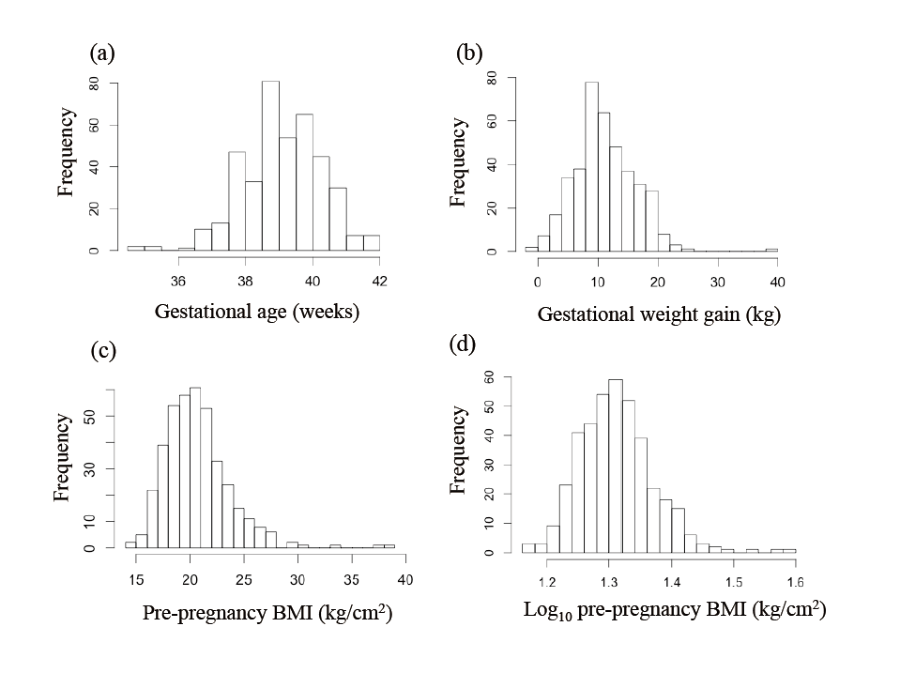
\includegraphics{Figures/Fig31.pdf}
\caption[Histograms of (a) gestational age, (b) gestational weight gain, (c) pre-pregnancy body mass index, and (d) $\log_{10}$ pre-pregnancy body mass index]{Histograms of (a) gestational age, (b) gestational weight gain, (c) prepregnancy body mass index (BMI), and (d) $\log_{10}$ pre-pregnancy BMI.}
\label{fig:Fig31}
\end{center}
\end{figure}


\begin{figure}
  \centering
  \label{fig:Fig32}
  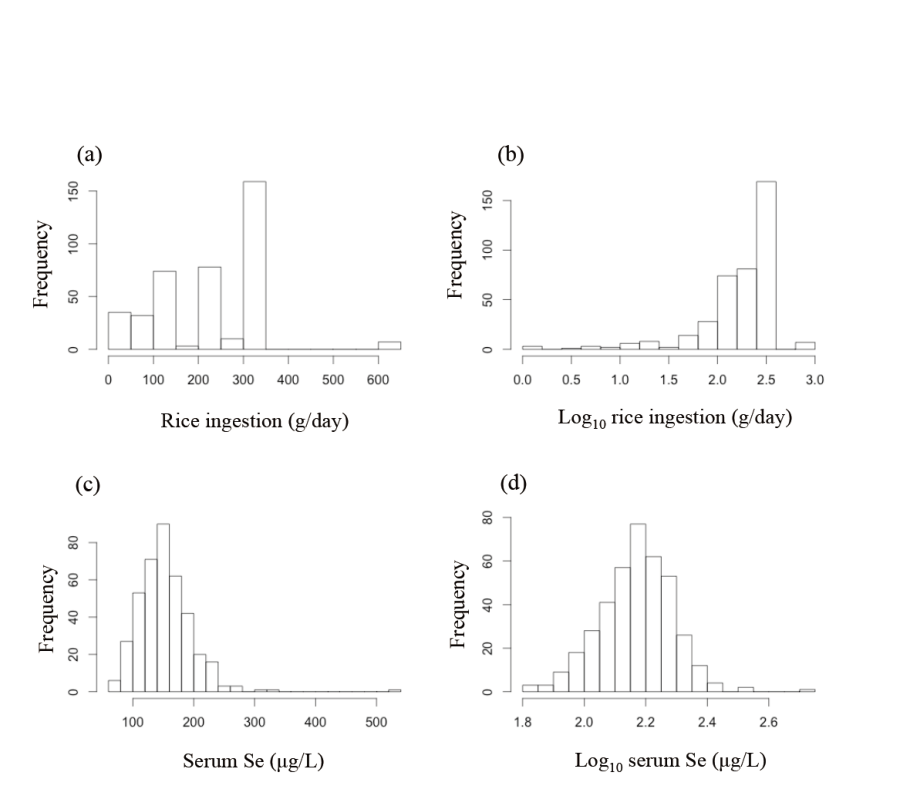
\includegraphics[scale=1]{Figures/Fig32.pdf}
  \caption[Histograms of (a) rice ingestion, (b) $\log_{10}$ rice ingestion, (c) serum selenium, and (4) $\log_{10}$ serum selenium]{Histograms of (a) rice ingestion, (b) $\log_{10}$ rice ingestion, (c) serum selenium (Se), and (4) $\log_{10}$ serum Se.}
\end{figure}

\begin{figure}
  \centering
    \label{fig:Fig33}
  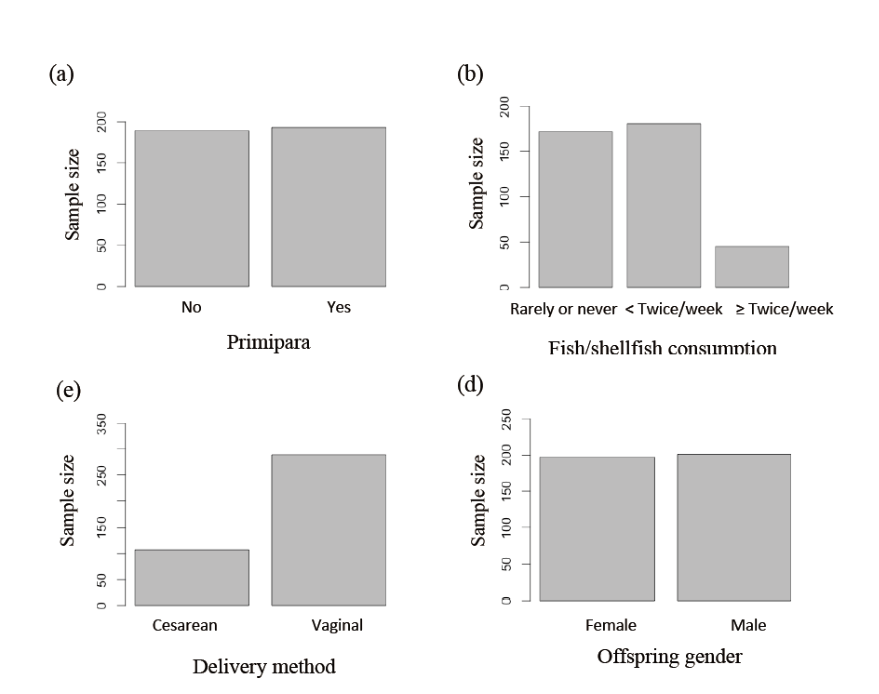
\includegraphics[scale=1]{Figures/Fig33.pdf}
  \caption[Distributions of (a) primipara, (b) fish/shellfish consumption, (c) delivery method, and (d) offspring gender]{Distributions of (a) primipara, (b) fish/shellfish consumption, (c) delivery method, and (d) offspring gender.}
\end{figure}

\begin{figure}
  \centering
    \label{fig:Fig34}
  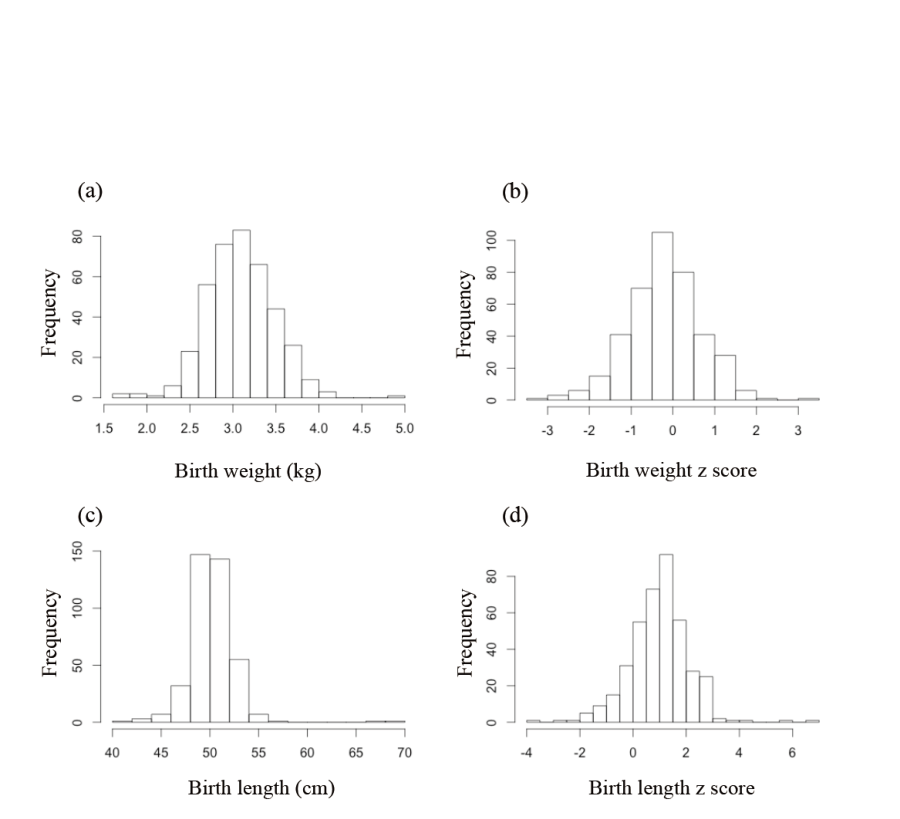
\includegraphics[scale=1]{Figures/Fig34.pdf}
  \caption[Histograms of (a) birth weight, (b) birth weight z score, (c) birth length, and (d) birth length z score]{Histograms of (a) birth weight, (b) birth weight z score, (c) birth length, and (d) birth length z score.}
\end{figure}

\begin{figure}
  \centering
    \label{fig:Fig35}
  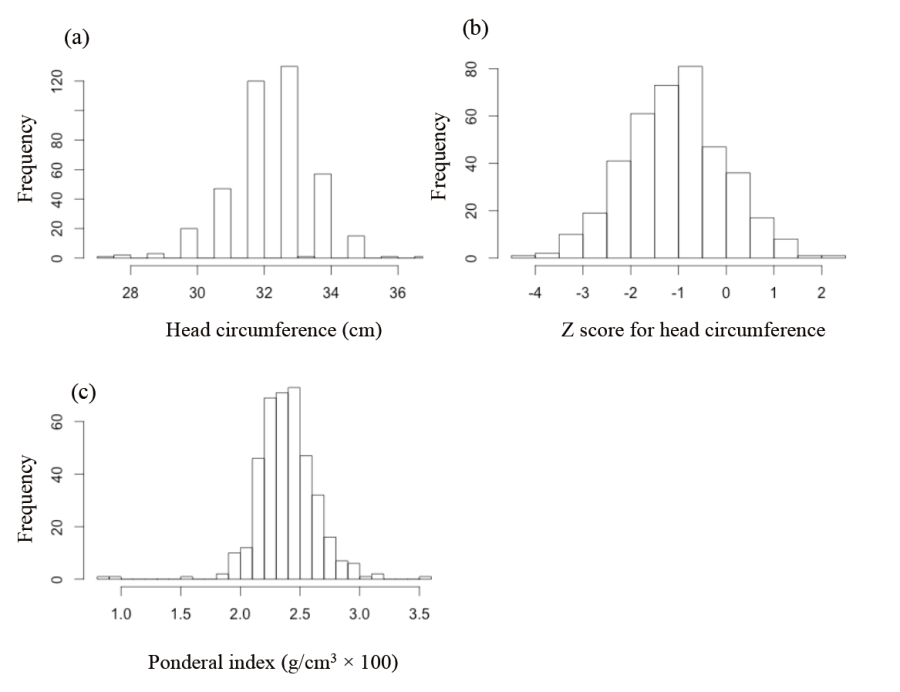
\includegraphics[scale=1]{Figures/Fig35.pdf}
  \caption[Histograms of (a) head circumference, (b) head circumference z score, and (c) ponderal index]{Histograms of (a) head circumference, (b) head circumference z score, and (c) ponderal index.}
\end{figure}

\begin{figure}
  \centering
    \label{fig:Fig36}
  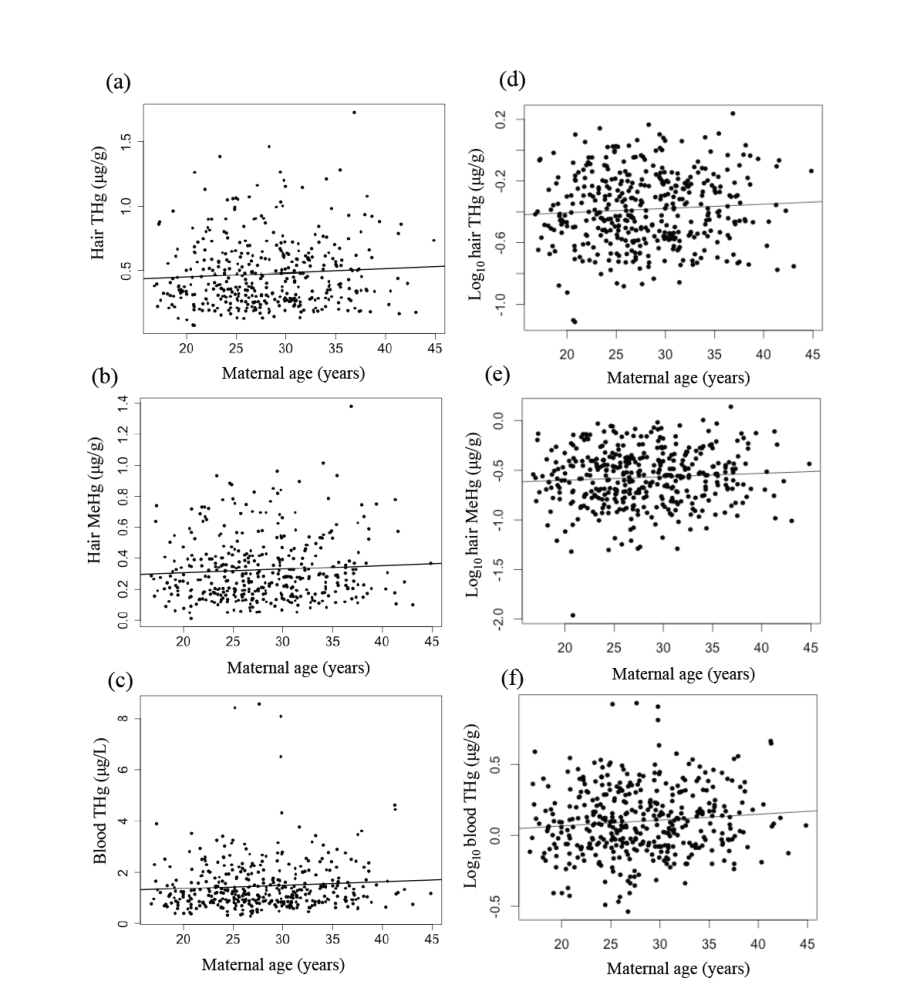
\includegraphics[scale=1]{Figures/Fig36.pdf}
  \caption[Bivariate analyses of maternal age versus mercury biomarkers]{Bivariate analyses of maternal age versus mercury biomarkers. Spearman's correlation test of maternal age versus (a) hair total mercury (THg) (rho=0.048, p=0.34), (b) hair methylmercury (MeHg) (rho=0.05, p=0.32), (c) blood THg (rho=0.087, p=0.08), and Pearson's correlation test of maternal age versus (d) $\log_{10}$ hair THg (rho=0.068, p=0.18), (e) $\log_{10}$ hair MeHg (rho=0.071, p=0.16), and (f) $\log_{10}$ blood THg (rho=0.099, p=0.06) (n=397-398 for all).}
\end{figure}

\begin{figure}
  \centering
    \label{fig:Fig37}
  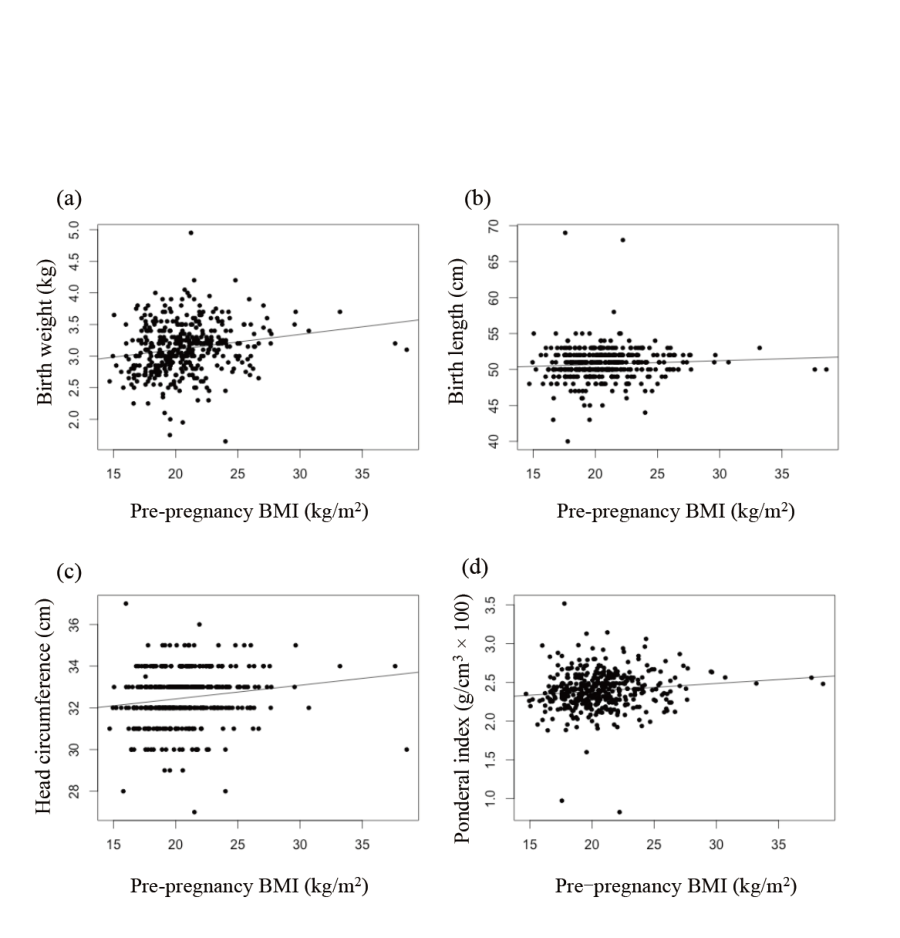
\includegraphics[scale=1]{Figures/Fig37.pdf}
  \caption[Bivariate analyses of pre-pregnancy body mass index versus birth outcomes]{Bivariate analyses of pre-pregnancy body mass index (BMI) versus birth outcomes. Spearman's correlation test of pre-pregnancy BMI versus (a) birth weight (rho = 0.21, p < 0.01), (b) birth length (rho = 0.12, p = 0.02), (c) head circumference (rho = 0.20, p < 0.01), and (d) ponderal index (rho = 0.14, p < 0.01) (Spearman's correlation test for all, n=397 for all).}
\end{figure}

\begin{figure}
  \centering
    \label{fig:Fig38}
  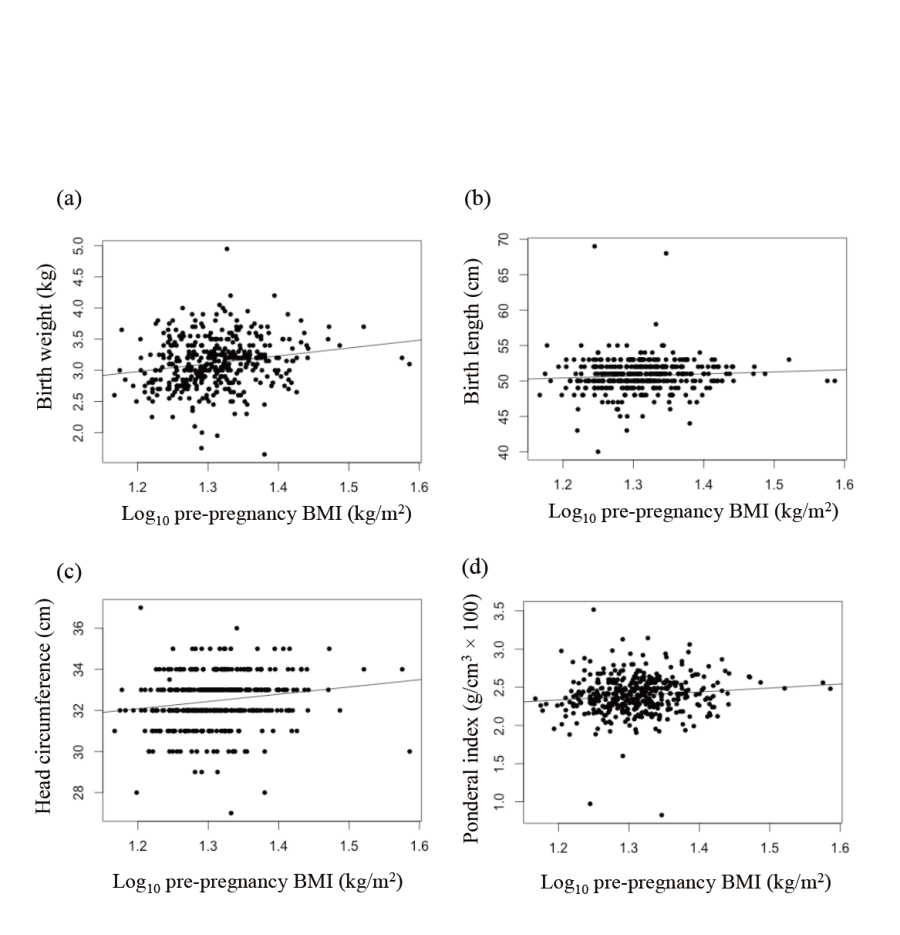
\includegraphics[scale=1]{Figures/Fig38.pdf}
  \caption[Bivariate analyses of $\log_{10}$  pre-pregnancy body mass index versus birth outcomes (birth weight, birth length, head circumference, ponderal index)]{Bivariate analyses of $\log_{10}$  pre-pregnancy body mass index (BMI) versus birth outcomes (birth weight, birth length, head circumference, ponderal index). Pearson's correlation test of $\log_{10}$  pre-pregnancy BMI versus (a) birth weight (rho = 0.19, p < 0.001), (b) birth length (rho = 0.073, p = 0.05), (c) head circumference (rho = 0.17, p < 0.001), and (d) ponderal index (rho = 0.12, p = 0.01) (Pearson's correlation test for all, n=397 for all).}
\end{figure}

\begin{figure}
  \centering
    \label{fig:Fig39}
  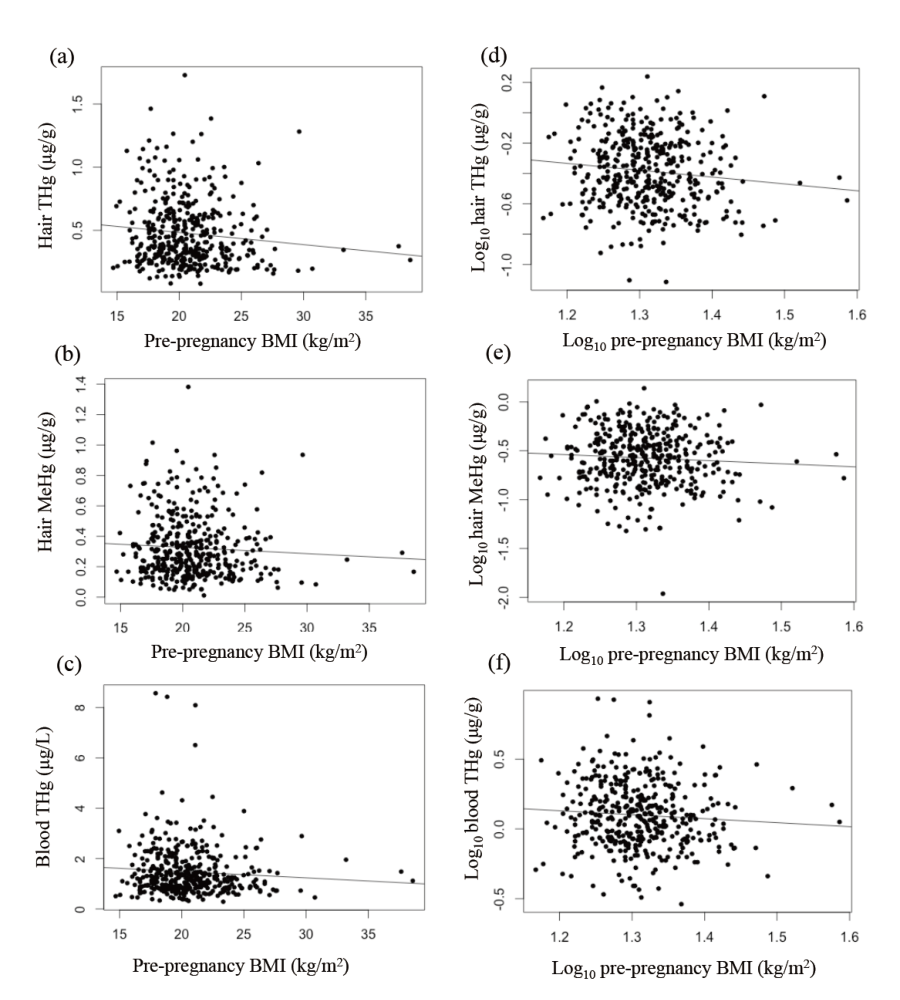
\includegraphics[scale=1]{Figures/Fig39.pdf}
  \caption[Bivariate analyses of pre-pregnancy body mass index versus mercury biomarkers]{Bivariate analyses of pre-pregnancy body mass index (BMI) versus mercury biomarkers. Spearman's correlation test of pre-pregnancy BMI versus (a) hair total mercury (THg) (rho = -0.11, p = 0.03), (b) hair methylmercury (MeHg) (rho = -0.05, p = 0.28), (c) blood THg (rho = -0.08, p = 0.09), and Pearson's correlation test of $\log_{10}$ pre-pregnancy BMI versus (a) $\log_{10}$ hair THg (rho = -0.12, p = 0.02), (b) $\log_{10}$ hair MeHg (rho = -0.07, p =0.18), (c) $\log_{10}$ blood THg (rho = -0.07, p = 0.15) (n=396-397 for all).}
\end{figure}

\begin{figure}
  \centering
    \label{fig:Fig310}
  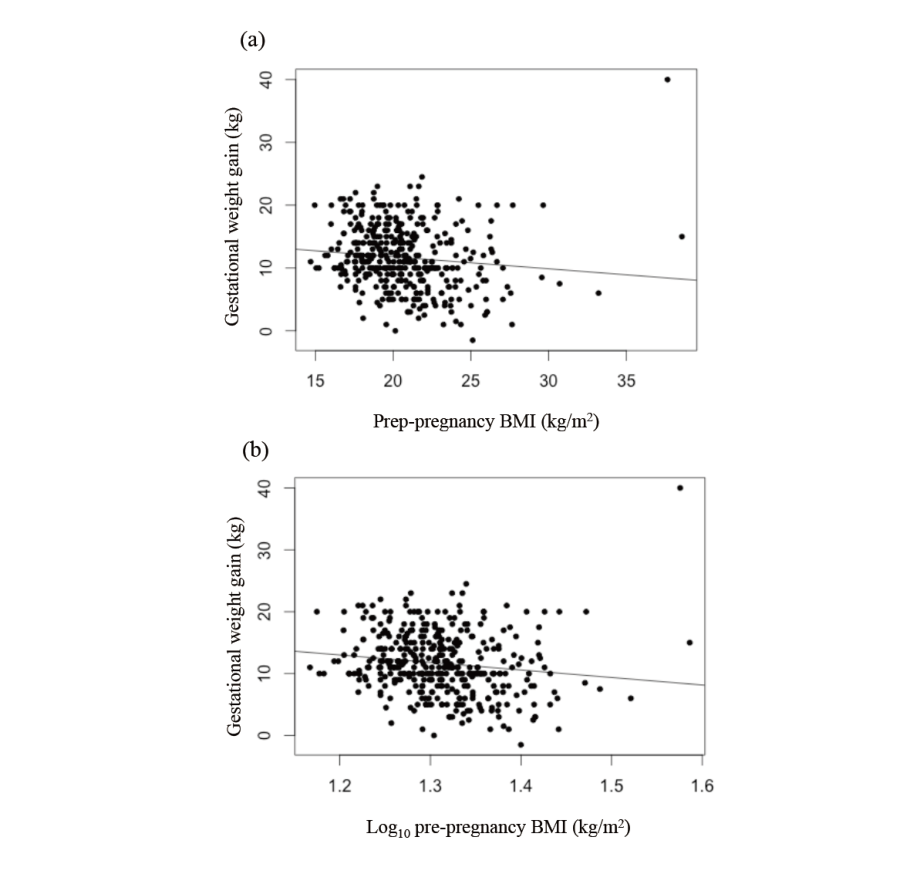
\includegraphics[scale=1]{Figures/Fig310.pdf}
  \caption[Bivariate analyses of gestational weight gain versus pre-pregnancy body mass index]{Bivariate analyses of gestational weight gain versus pre-pregnancy body mass index (BMI). (a) Gestational weight gain versus pre-pregnancy BMI (Spearman's rho = -0.23, p < 0.0001) and (b) gestational weight gain versus $\log_{10}$ pre-pregnancy BMI (Pearson's rho = -0.14, p = 0.004) (n=397 for all).}
\end{figure}

\begin{figure}
  \centering
    \label{fig:Fig311}
  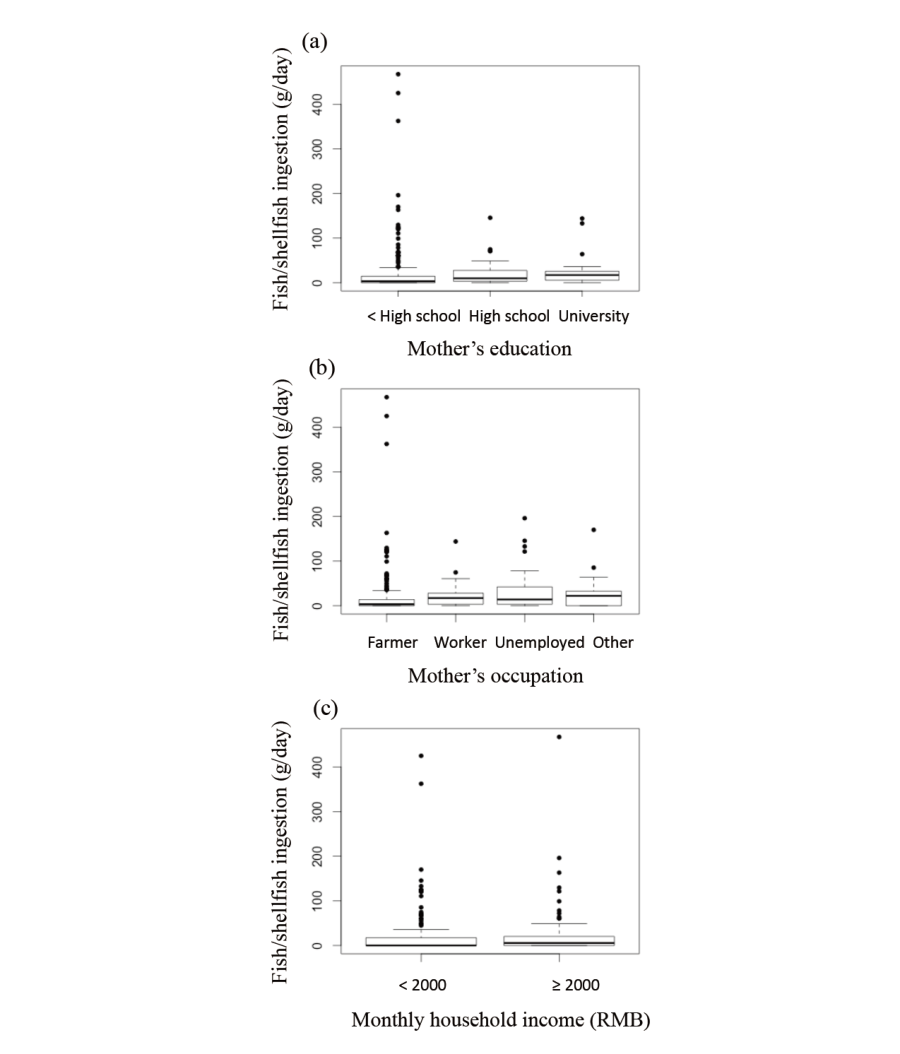
\includegraphics[scale=1]{Figures/Fig311.pdf}
  \caption[Bivariate analyses of fish/shellfish ingestion versus maternal characteristics (education, occupation, household income)]{Bivariate analyses of fish/shellfish ingestion versus maternal characteristics (education, occupation, household income). Fish/shellfish ingestion versus (a) mother's education (Kruskal-Wallis test, p < 0.01, n = 388), (b) mother's occupation (Kruskal-Wallis test, p < 0.01, n = 391), and (c) monthly household income (Wilcoxon-Mann-Whitney test, p = 0.03, n=363).}
\end{figure}

\begin{figure}
  \centering
    \label{fig:Fig312}
  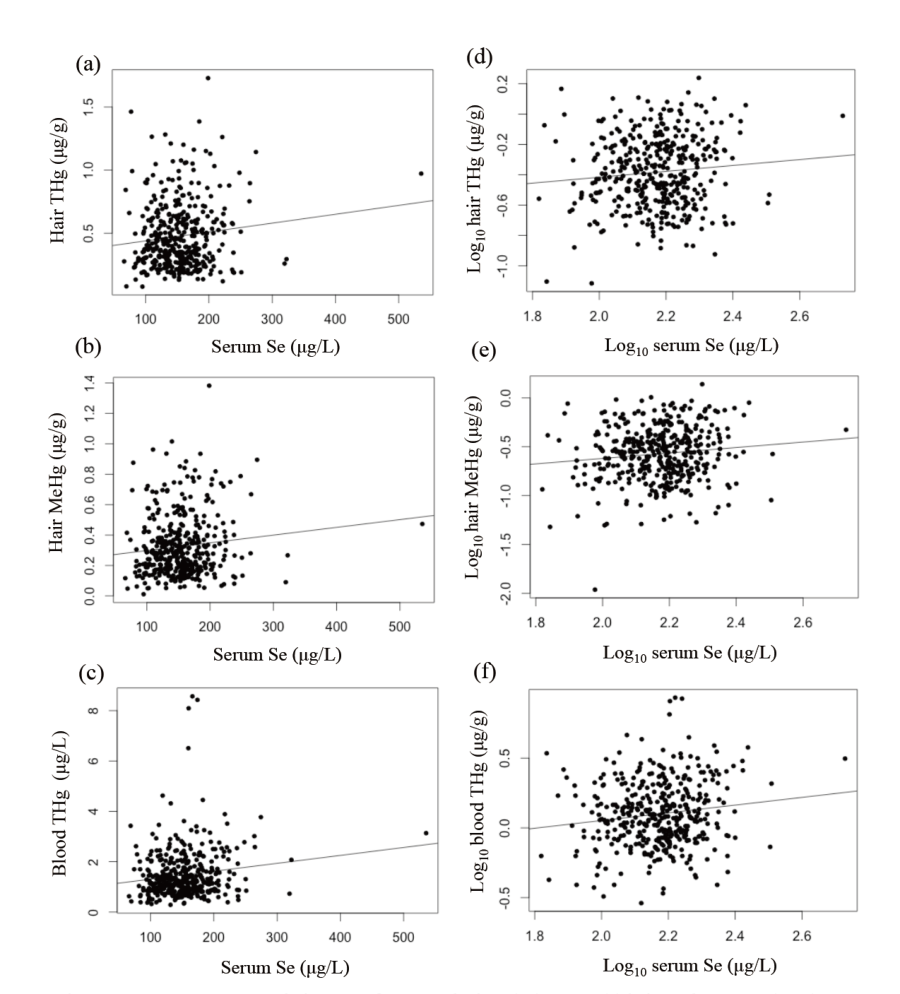
\includegraphics[scale=1]{Figures/Fig312.pdf}
  \caption[Bivariate analyses of serum selenium versus mercury biomarkers]{Bivariate analyses of serum selenium (Se) versus mercury biomarkers. Spearman's correlation test of serum Se versus (a) hair total mercury (THg) (rho = 0.06, p = 0.20), (b) hair methylmercury (MeHg) (rho = 0.09, p = 0.09), (c) blood THg (rho = 0.10, p = 0.04), and Pearson's correlation test of $\log_{10}$ serum Se versus (a) $\log_{10}$ hair THg (rho = 0.10, p = 0.08), (b) $\log_{10}$ hair MeHg (rho = 0.12, p =0.06), (c) $\log_{10}$ blood THg (rho = 0.14, p = 0.05) (n=396 for all).}
\end{figure}

\begin{figure}
  \centering
    \label{fig:Fig313}
  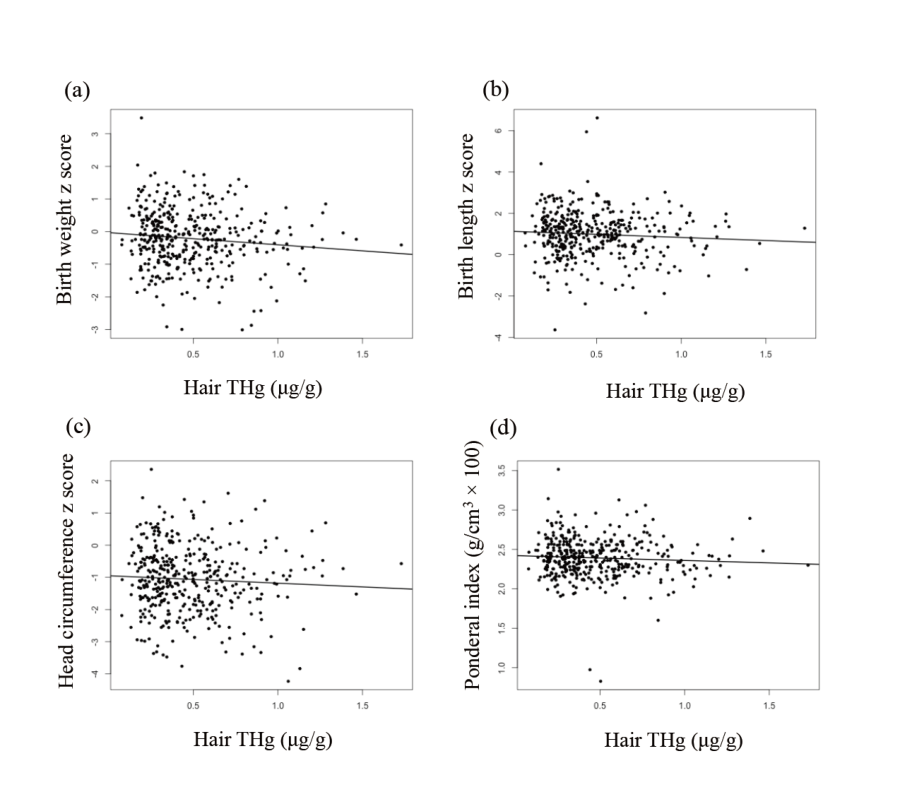
\includegraphics[scale=1]{Figures/Fig313.pdf}
  \caption[Bivariate analyses of hair total mercury versus birth outcomes (birth weight z score, birth length z score, head circumference z score, ponderal index)]{Bivariate analyses of hair total mercury (THg) versus birth outcomes (birth weight z score, birth length z score, head circumference z score, ponderal index). Spearman's correlation test of hair THg versus (a) birth weight z score (rho = -0.11, p = 0.04), (b) birth length z score (rho = -0.07, p = 0.19), (c) head circumference z score (rho = -0.07, p = 0.15), and (d) ponderal index (rho = -0.07, p = 0.15) (n=398 for all).}
\end{figure}


\begin{figure}
  \centering
    \label{fig:Fig314}
  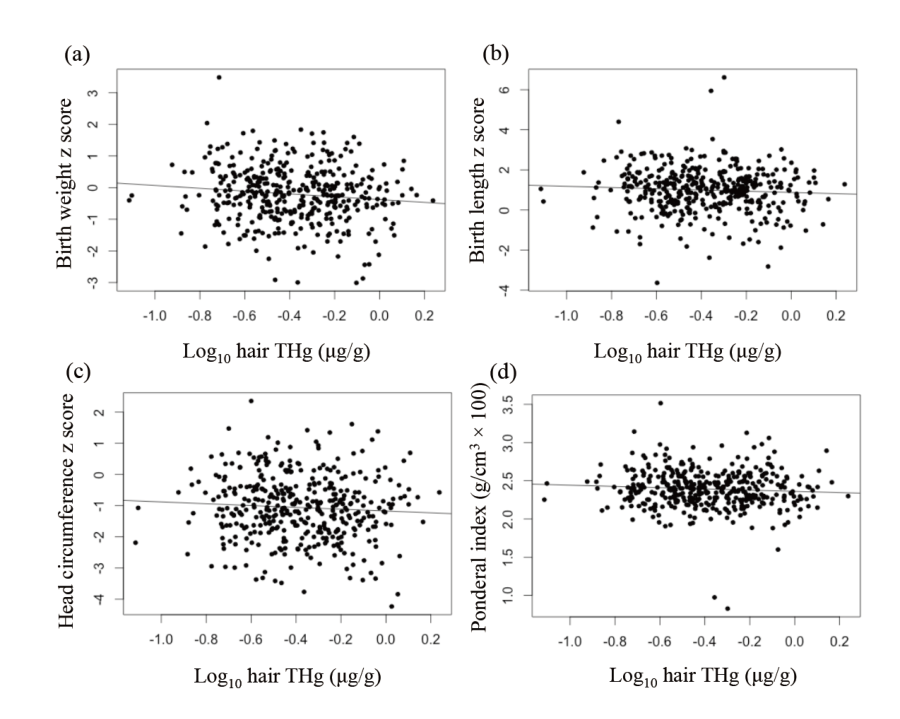
\includegraphics[scale=1]{Figures/Fig314.pdf}
  \caption[Bivariate analyses of $\log_{10}$ hair total mercury versus birth outcomes (birth weight z score, birth length z score, head circumference z score, ponderal index)]{Bivariate analyses of $\log_{10}$ hair total mercury (THg) versus birth outcomes (birth weight z score, birth length z score, head circumference z score, ponderal index). Pearson's correlation test of $\log_{10}$ hair THg versus (a) birth weight z score (rho = -0.12, p = 0.02), (b) birth length z score (rho = -0.07, p = 0.19), (c) head circumference z score (rho = -0.07, p = 0.19), and (d) ponderal index (rho = -0.08, p = 0.13) (n=398 for all).}
\end{figure}


\begin{figure}
  \centering
    \label{fig:Fig315}
  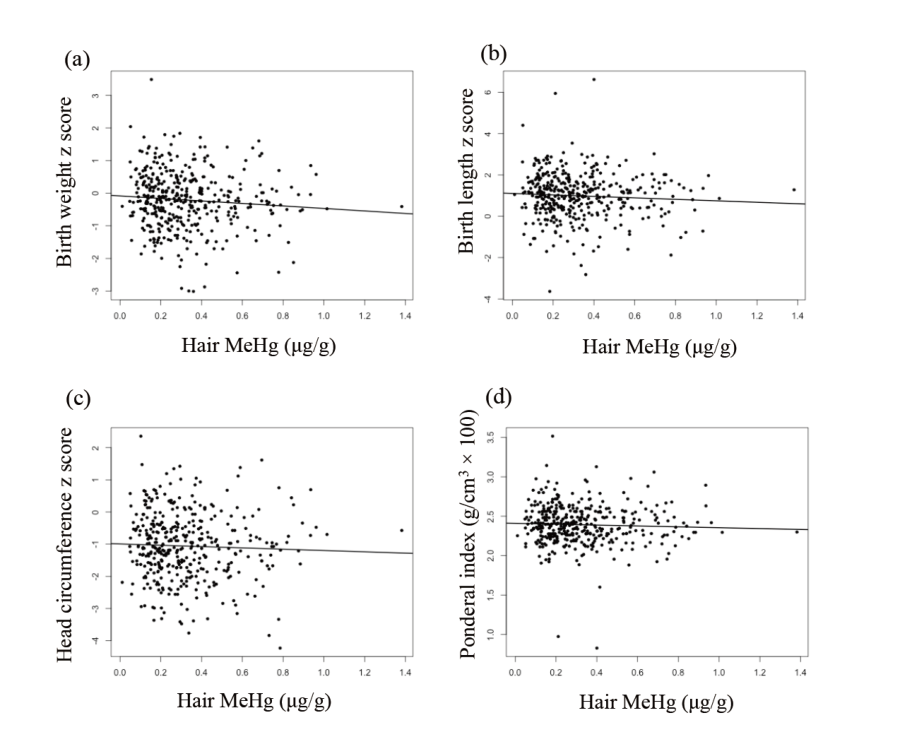
\includegraphics[scale=1]{Figures/Fig315.pdf}
  \caption[Bivariate analyses of hair methylmercury versus birth outcomes (birth weight z score, birth length z score, head circumference z score, ponderal index)]{Bivariate analyses of hair methylmercury (MeHg) versus birth outcomes (birth weight z score, birth length z score, head circumference z score, ponderal index). Spearman's correlation test of hair MeHg versus (a) birth weight z score (rho = -0.10, p = 0.05), (b) birth length z score (rho = -0.07, p = 0.16), (c) head circumference z score (rho = -0.07, p = 0.19), and (d) ponderal index (rho = -0.07, p=0.19) (n=398 for all).}
\end{figure}


\begin{figure}
  \centering
    \label{fig:Fig316}
  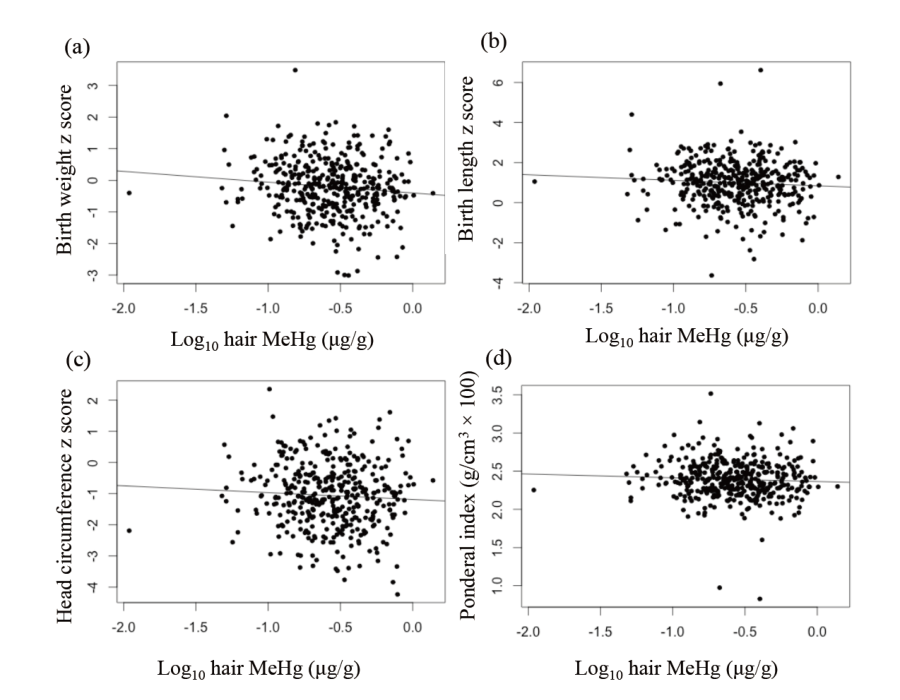
\includegraphics[scale=1]{Figures/Fig316.pdf}
  \caption[Bivariate analyses of $\log_{10}$ hair methylmercury versus birth outcomes (birth weight z score, birth length z score, head circumference z score, ponderal index)]{Bivariate analyses of $\log_{10}$ hair methylmercury (MeHg) versus birth outcomes (birth weight z score, birth length z score, head circumference z score, ponderal index). Pearson's correlation test of $\log_{10}$ hair MeHg versus (a) birth weight z score (rho = -0.11, p = 0.03), (b) birth length z score (rho = -0.07, p = 0.16), (c) head circumference z score (rho = -0.06, p = 0.24), and (d) ponderal index (rho = -0.06, p=0.27) (n=398 for
all).}
\end{figure}

\begin{figure}
  \centering
    \label{fig:Fig317}
  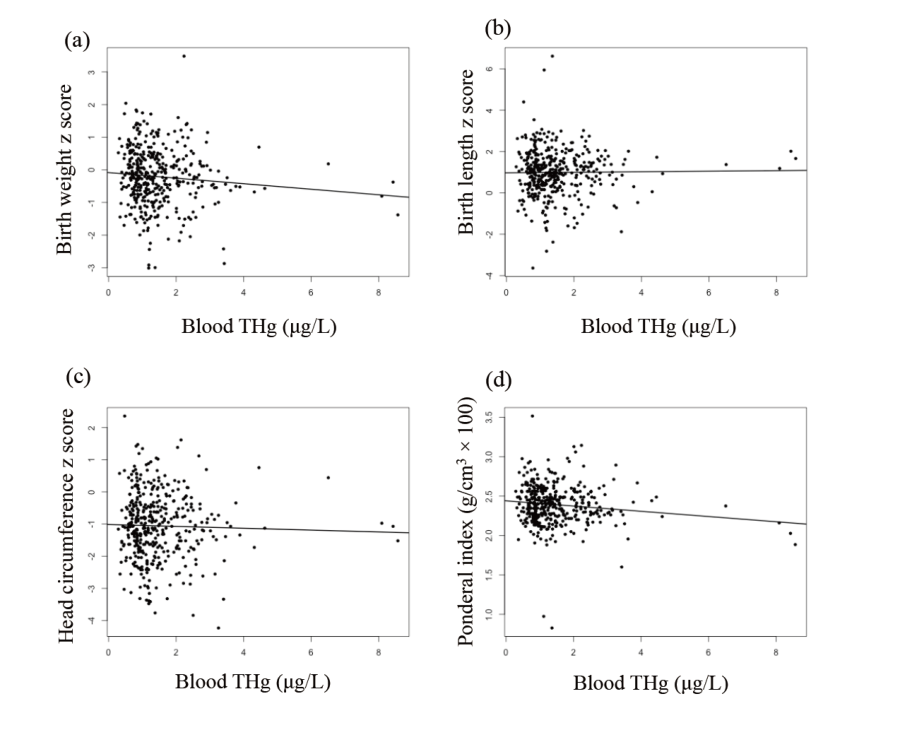
\includegraphics[scale=1]{Figures/Fig317.pdf}
  \caption[Bivariate analyses of blood total mercury versus birth outcomes (birth weight z score, birth length z score, head circumference z score, ponderal index)]{Bivariate analyses of blood total mercury (THg) versus birth outcomes (birth weight z score, birth length z score, head circumference z score, ponderal index). Spearman's correlation test of blood THg versus (a) birth weight z score (rho = -0.10, p = 0.05), (b) birth length z score (rho = 0.0014, p=0.98), (c) head circumference z score (rho = -0.03, p=0.54), and (d) ponderal index (rho = -0.11, p = 0.03) (n=397 for all).}
\end{figure}


\begin{figure}
  \centering
    \label{fig:Fig318}
  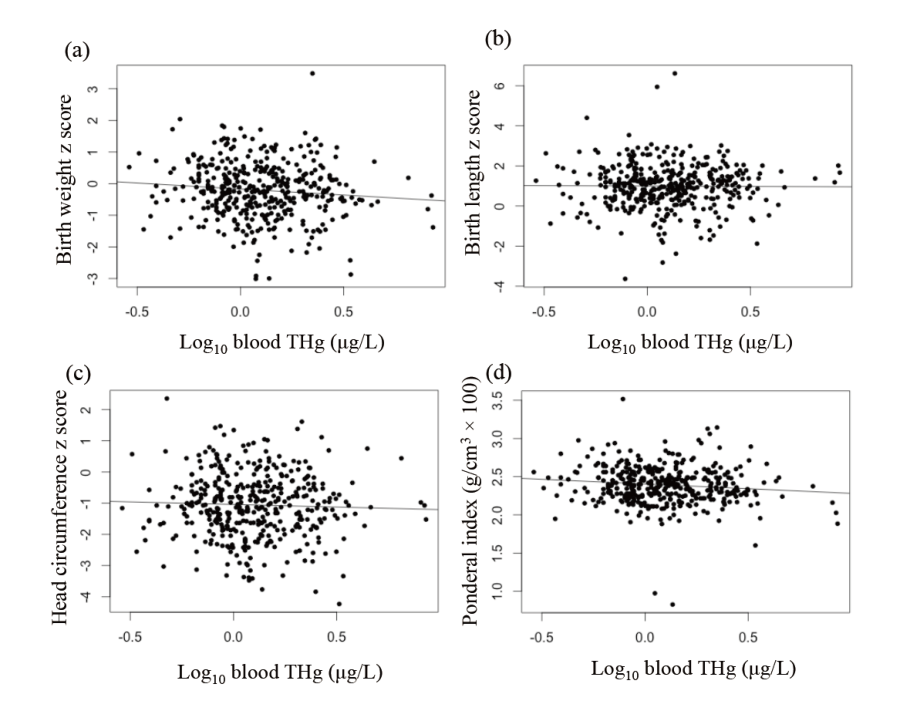
\includegraphics[scale=1]{Figures/Fig318.pdf}
  \caption[Bivariate analyses of $\log_{10}$ blood total mercury versus birth outcomes (birth weight z score, birth length z score, head circumference z score, ponderal index)]{Bivariate analyses of $\log_{10}$ blood total mercury (THg) versus birth outcomes (birth weight z score, birth length z score, head circumference z score, ponderal index). Pearson's correlation test of $\log_{10}$ blood THg versus (a) birth weight z score (rho = -0.10, p = 0.04), (b) birth length z score (rho = 0.0092, p=0.85), (c) head circumference z score (rho = -0.04, p=0.45), and (d) ponderal index (rho = -0.12, p = 0.02) (n=397 for all).}
\end{figure}


\begin{figure}
  \centering
    \label{fig:Fig319}
  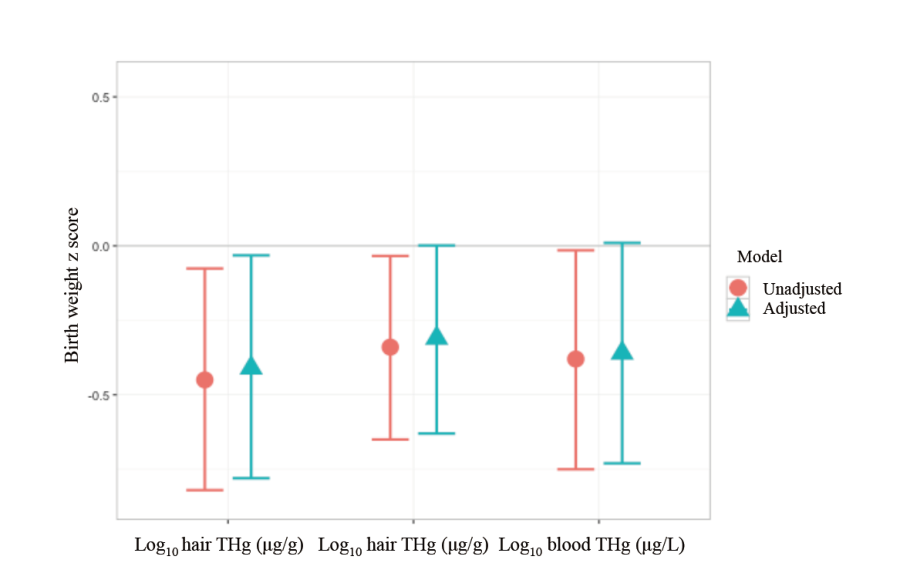
\includegraphics[scale=1]{Figures/Fig319.pdf}
  \caption[Betas and 95\% confidence intervals for birth weight z score related to $\log_{10}$ hair total mercury, $\log_{10}$ hair methylmercury, and $\log_{10}$ blood total mercury in unadjusted and adjusted models]{Betas and 95\% confidence intervals (CIs) for birth weight z score related to $\log_{10}$ hair total mercury (THg), $\log_{10}$ hair methylmercury (MeHg), and $\log_{10}$ blood THg in unadjusted and adjusted models.}
\end{figure}


\begin{figure}
  \centering
    \label{fig:Fig320}
  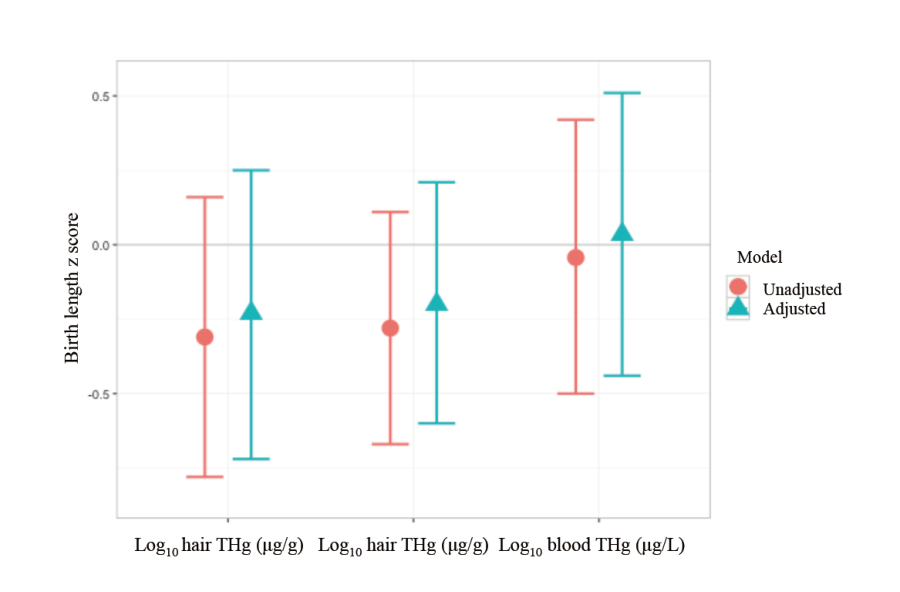
\includegraphics[scale=1]{Figures/Fig320.pdf}
  \caption[Betas and 95\% confidence intervals for birth length z score related to $\log_{10}$ hair total mercury, $\log_{10}$ hair methylmercury, and $\log_{10}$ blood  total mercury in unadjusted and adjusted models]{Betas and 95\% confidence intervals (CIs) for birth length z score related to $\log_{10}$ hair total mercury (THg), $\log_{10}$ hair methylmercury (MeHg), and $\log_{10}$ blood THg in unadjusted and adjusted models.}
\end{figure}


\begin{figure}
  \centering
    \label{fig:Fig321}
  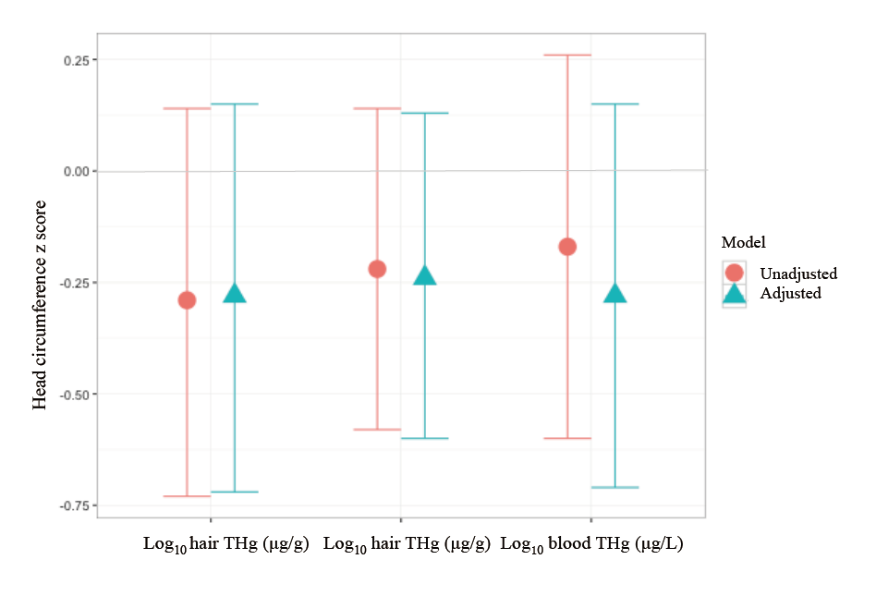
\includegraphics[scale=1]{Figures/Fig321.pdf}
  \caption[Betas and 95\% confidence intervals for head circumference z score related to $\log_{10}$ hair total mercury, $\log_{10}$ hair methylmercury, and $\log_{10}$ blood total mercury in unadjusted and adjusted models]{Betas and 95\% confidence intervals (CIs) for head circumference z score related to $\log_{10}$ hair total mercury (THg), $\log_{10}$ hair methylmercury (MeHg), and $\log_{10}$ blood THg in unadjusted and adjusted models.}
\end{figure}


\begin{figure}
  \centering
    \label{fig:Fig322}
  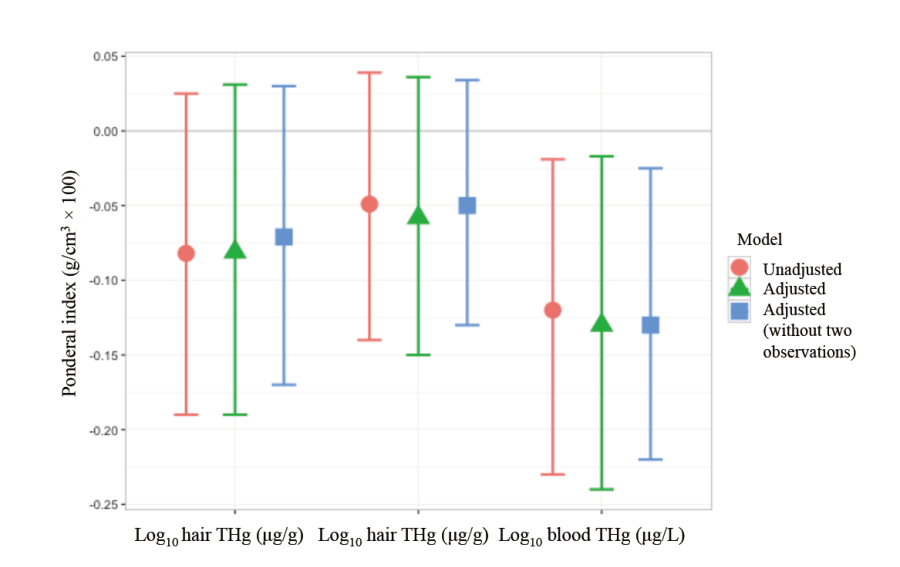
\includegraphics[scale=1]{Figures/Fig322.pdf}
  \caption[Betas and 95\% confidence intervals for ponderal index related to $\log_{10}$ hair total mercury, $\log_{10}$ hair methylmercury, and $\log_{10}$ blood total mercury in unadjusted and adjusted models (with and without two outliers)]{Betas and 95\% confidence intervals (CIs) for ponderal index related to $\log_{10}$ hair total mercury (THg), $\log_{10}$ hair methylmercury (MeHg), and $\log_{10}$ blood THg in unadjusted and adjusted models (with and without two outliers).}
\end{figure}


\begin{figure}
  \centering
    \label{fig:Fig323}
  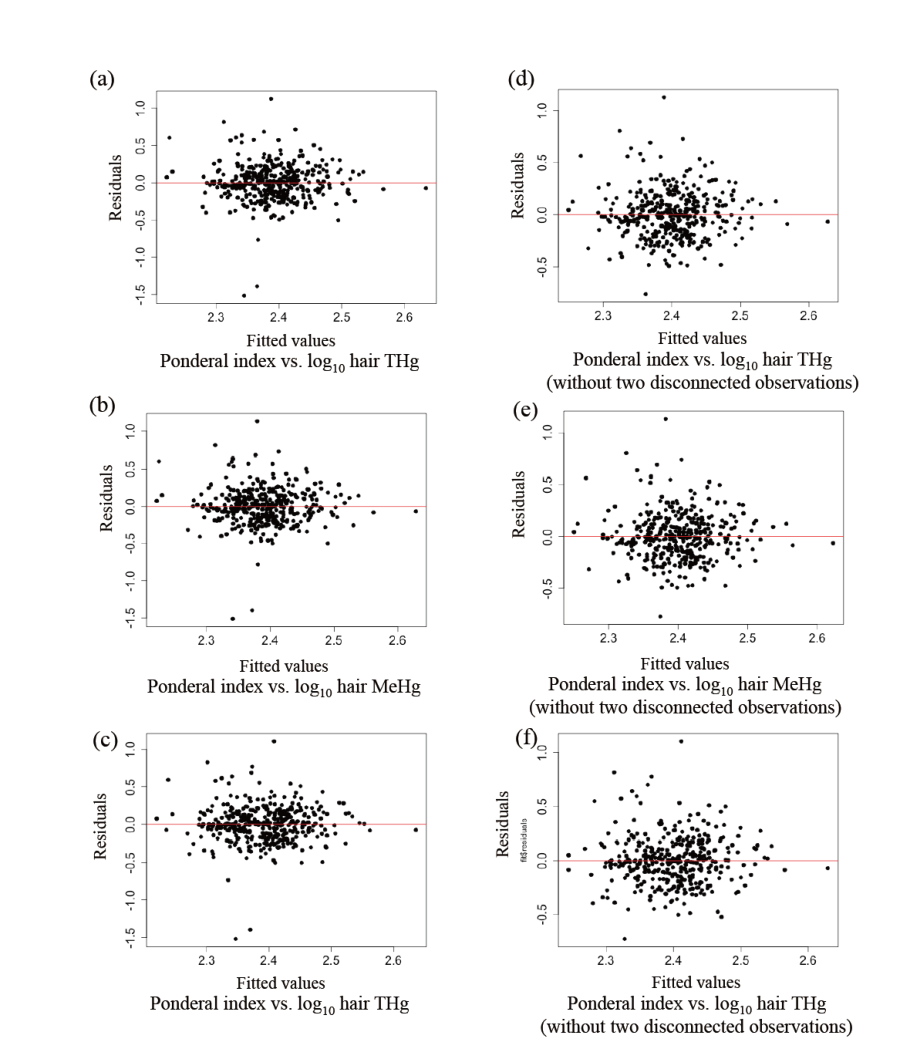
\includegraphics[scale=1]{Figures/Fig323.pdf}
  \caption[Residuals versus fitted values plots of multiple linear regression models]{Residuals versus fitted values plots of multiple linear regression models. (a) and (d) for ponderal index versus $\log_{10}$ hair total mercury (THg), (b) and (e) for ponderal index versus $\log_{10}$ methylmercury (MeHg), (c) and (f) for ponderal index versus $\log_{10}$ blood THg. (a)-(c) for all participant, and (d)-(f) for participants without two disconnected observations.}
\end{figure}


\begin{figure}
  \centering
    \label{fig:Fig324}
  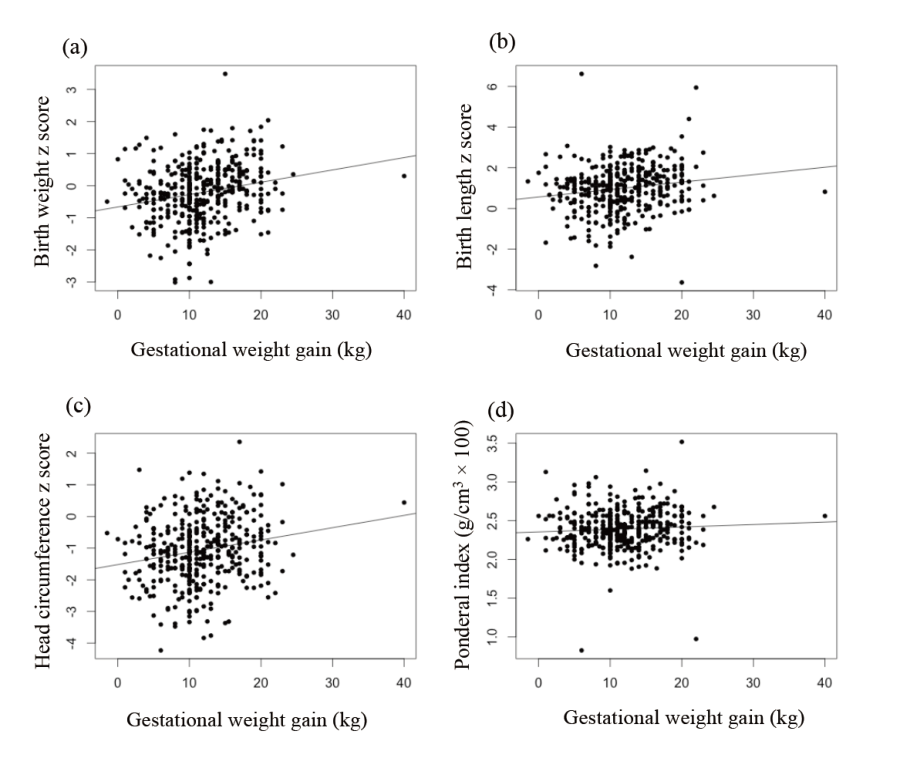
\includegraphics[scale=1]{Figures/Fig324.pdf}
  \caption[Bivariate analyses of maternal gestational weight gain versus birth outcomes (birth weight z score, birth length z score, head circumference z score, ponderal index)]{Bivariate analyses of maternal gestational weight gain versus birth outcomes (birth weight z score, birth length z score, head circumference z score, ponderal index). Pearson's correlation test of gestational weight gain versus (a) birth weight z score (rho = 0.22, p < 0.0001), (b) birth length z score (rho = 0.17, p < 0.001), (c) head circumference z score (rho = 0.19, p < 0.001), (d) ponderal index (rho = 0.06, p = 0.20) (n=397 for all).}
\end{figure}


\begin{figure}
  \centering
    \label{fig:Fig325}
  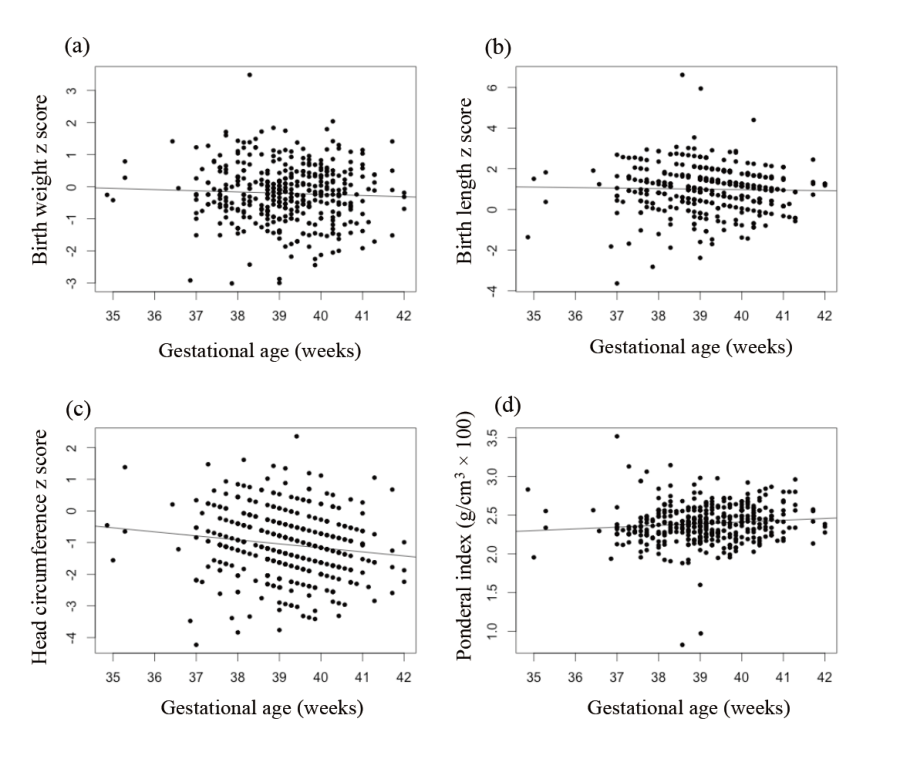
\includegraphics[scale=1]{Figures/Fig325.pdf}
  \caption[Bivariate analyses of gestational age versus birth outcomes (birth weight z score, birth length z score, head circumference z score, ponderal index)]{Bivariate analyses of gestational age versus birth outcomes (birth weight z score, birth length z score, head circumference z score, ponderal index). Pearson's correlation test of gestational age versus (a) birth weight z score (rho = -0.05, p = 0.33), (b) birth length z score (rho = -0.03, p = 0.59), (c) head circumference z score (rho = -0.14, p = 0.004), (d) ponderal index (rho = 0.10, p = 0.04) (n=398 for all).}
\end{figure}


\begin{figure}
  \centering
    \label{fig:Fig326}
  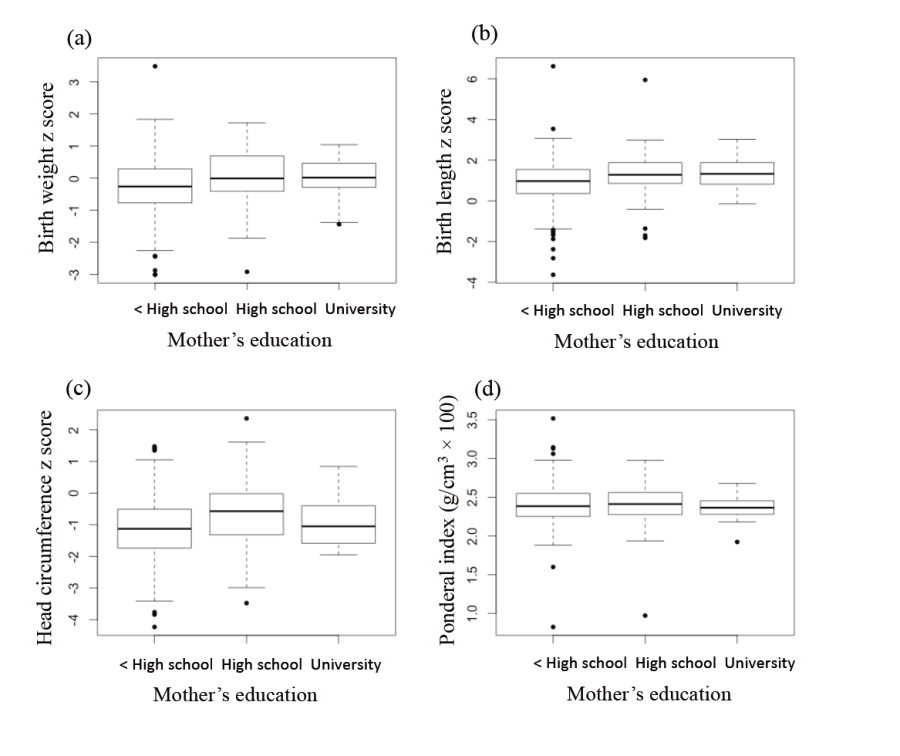
\includegraphics[scale=1]{Figures/Fig326.pdf}
  \caption[Bivariate analyses of mother's education versus birth outcomes (birth weight z score, birth length z score, head circumference z score, ponderal index)]{Bivariate analyses of mother's education versus birth outcomes (birth weight z score, birth length z score, head circumference z score, ponderal index). One-way ANOVA test of mother's education versus (a) birth weight z score (p = 0.08), (b) birth length z score (p = 0.04), (c) head circumference z score (p = 0.02), (d) ponderal index (p = 0.90) (n=388 for all).}
\end{figure}


\begin{figure}
  \centering
    \label{fig:Fig327}
  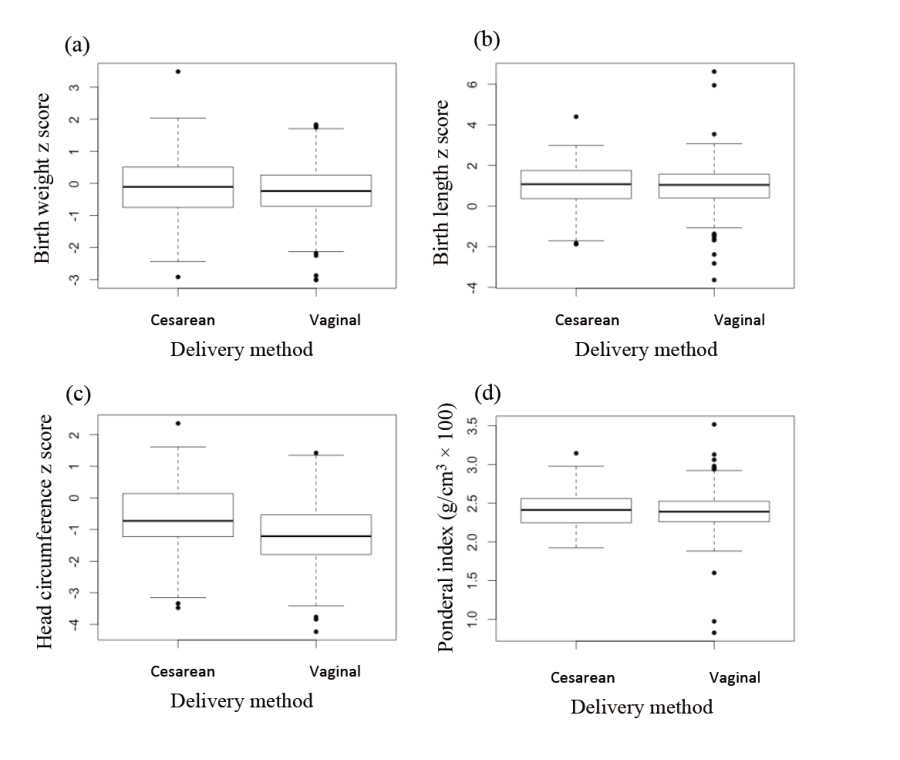
\includegraphics[scale=1]{Figures/Fig327.pdf}
  \caption[Bivariate analyses of delivery method versus birth outcomes (birth weight z score, birth length z score, head circumference z score, ponderal index)]{Bivariate analyses of delivery method versus birth outcomes (birth weight z score, birth length z score, head circumference z score, ponderal index). Student's t-test of delivery method versus (a) birth weight z score (p = 0.17), (b) birth length z score (p = 0.59), (c) head circumference z score (p < 0.01), (d) ponderal index (p = 0.70) (n=398 for all).}
\end{figure}

\begin{figure}
  \centering
    \label{fig:Fig328}
  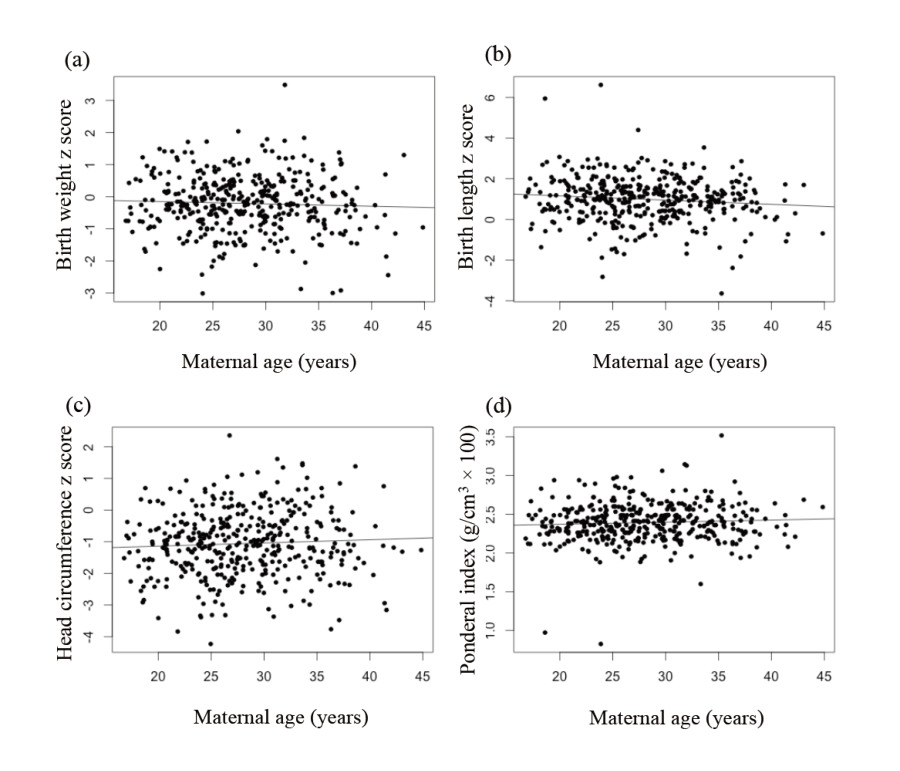
\includegraphics[scale=1]{Figures/Fig328.pdf}
  \caption[Bivariate analyses of maternal age versus birth outcomes (birth weight z score, birth length z score, head circumference z score, ponderal index)]{Bivariate analyses of maternal age versus birth outcomes (birth weight z score, birth length z score, head circumference z score, ponderal index). Pearson's correlation test of maternal age versus (a) birth weight z score (rho = -0.05, p = 0.35), (b) birth length z score (rho = -0.11, p = 0.13), (c) head circumference z score (rho = 0.06, p=0.27), and (d) ponderal index (rho = 0.06, p = 0.22) (n=398 for all).}
\end{figure}

\begin{figure}
  \centering
    \label{fig:Fig329}
  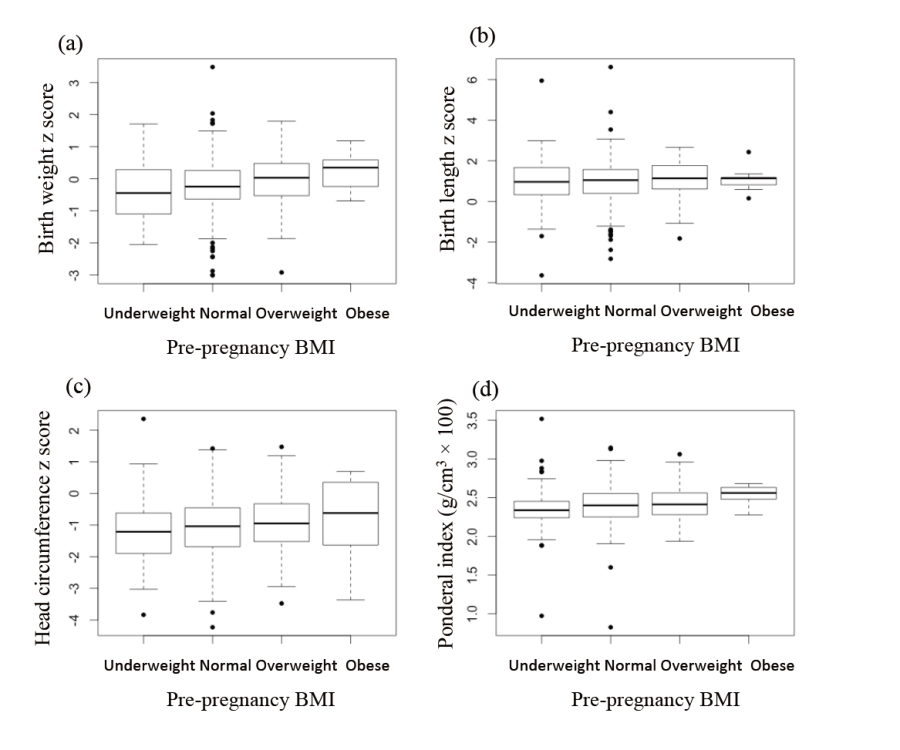
\includegraphics[scale=1]{Figures/Fig329.pdf}
  \caption[Bivariate analyses of maternal pre-pregnancy body mass index versus birth outcomes (birth weight z score, birth length z score, head circumference z score, ponderal index)]{Bivariate analyses of maternal pre-pregnancy body mass index (BMI) versus birth outcomes (birth weight z score, birth length z score, head circumference z score, ponderal index). One-way ANOVA test of pre-pregnancy BMI versus (a) birth weight z score (p = 0.11), (b) birth length z score (p = 0.97), (c) head circumference z score (p = 0.28), (d) ponderal index (p = 0.10) (n=397 for all).}
\end{figure}

\begin{figure}
  \centering
    \label{fig:Fig330}
  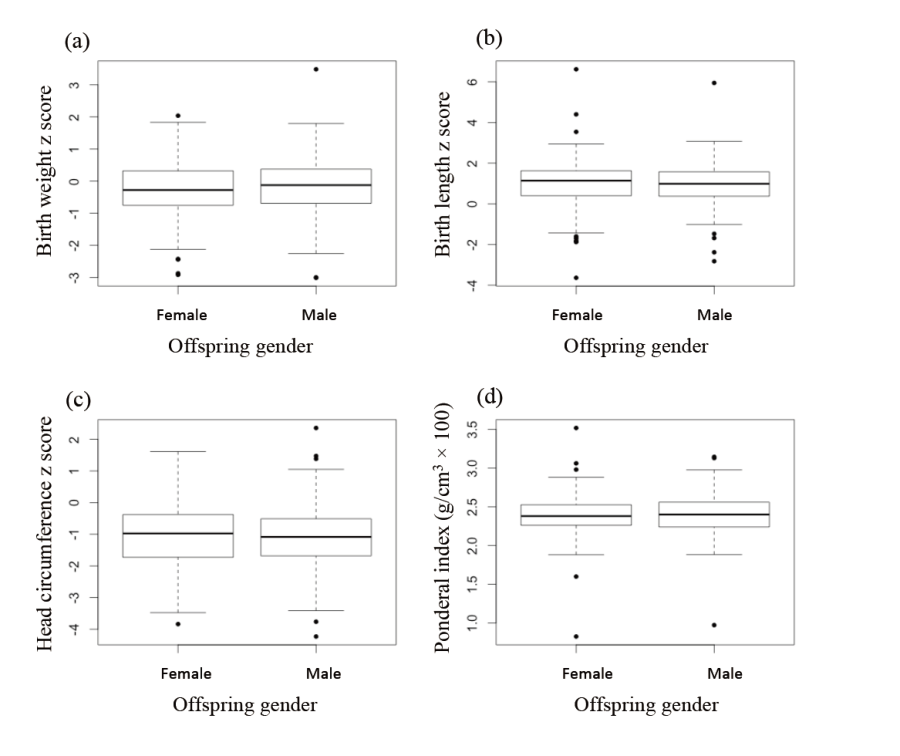
\includegraphics[scale=1]{Figures/Fig330.pdf}
  \caption[Bivariate analyses of offspring gender versus birth outcomes (birth weight z score, birth length z score, head circumference z score, ponderal index)]{Bivariate analyses of offspring gender versus birth outcomes (birth weight z score, birth length z score, head circumference z score, ponderal index). Student's t-test of offspring gender versus (a) birth weight z score (p = 0.30), (b) birth length z score (p = 0.66), (c) head circumference z score (p = 0.65), (d) ponderal index (p = 0.60) (n=398 for all).}
\end{figure}

\begin{figure}
  \centering
    \label{fig:Fig331}
  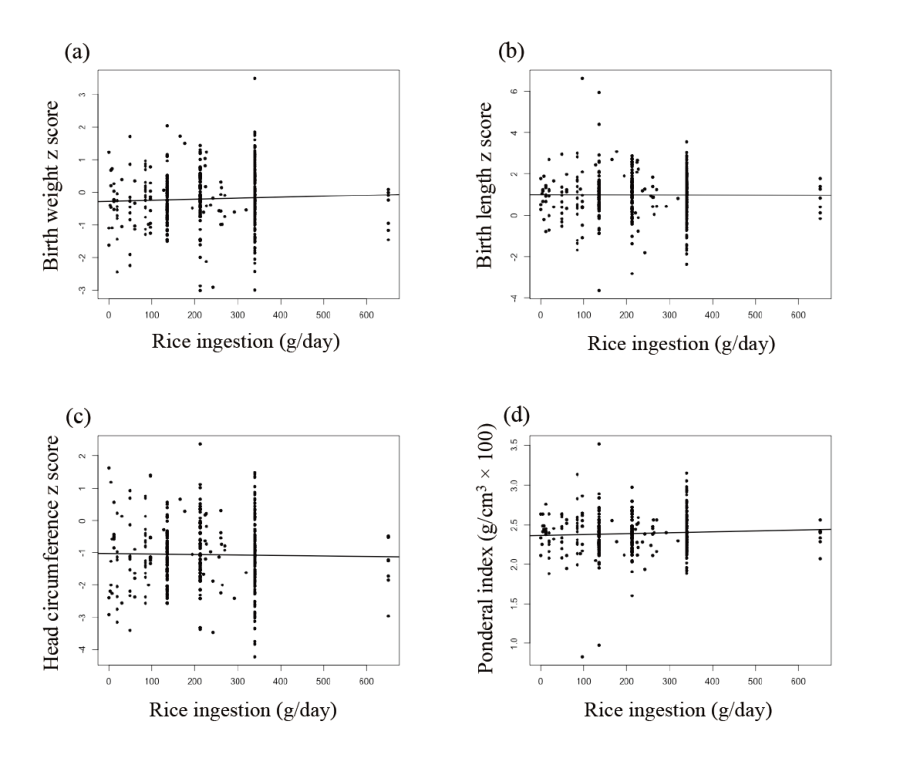
\includegraphics[scale=1]{Figures/Fig331.pdf}
  \caption[Bivariate analyses of rice ingestion versus birth outcomes (birth weight z score, birth length z score, head circumference z score, ponderal index)]{Bivariate analyses of rice ingestion versus birth outcomes (birth weight z score, birth length z score, head circumference z score, ponderal index). Spearman's correlation test of rice ingestion versus (a) birth weight z score (rho = 0.06, p = 0.20), (b) birth length z score (rho = 0.03, p = 0.55), (c) head circumference z score (rho = 0.01, p = 0.82), (d) ponderal index (rho = 0.04, p = 0.41) (n=398 for all).}
\end{figure}

\begin{figure}
  \centering
    \label{fig:Fig332}
  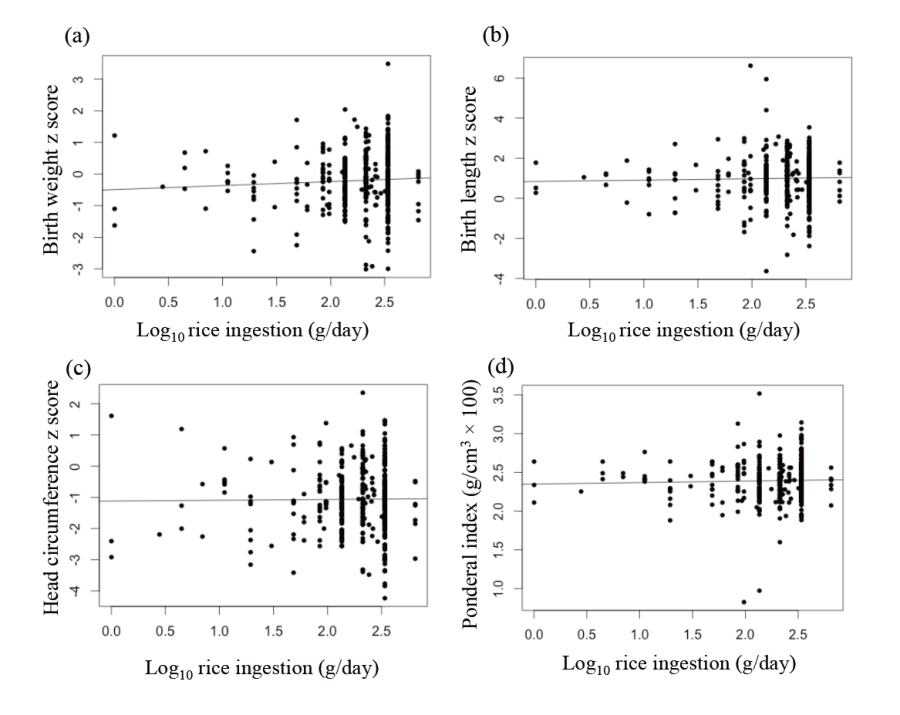
\includegraphics[scale=1]{Figures/Fig332.pdf}
  \caption[Bivariate analyses of $\log_{10}$ rice ingestion versus birth outcomes (birth weight z score, birth length z score, head circumference z score, ponderal index)]{Bivariate analyses of $\log_{10}$ rice ingestion versus birth outcomes (birth weight z score, birth length z score, head circumference z score, ponderal index). Pearson's correlation test of $\log_{10}$ rice ingestion versus (a) birth weight z score (rho = 0.06, p = 0.23), (b) birth length z score (rho = 0.03, p = 0.61), (c) head circumference z score (rho = 0.01, p = 0.84), (d) ponderal index (rho = 0.03, p = 0.52) (n=398 for all).}
\end{figure}

\begin{figure}
  \centering
    \label{fig:Fig333}
  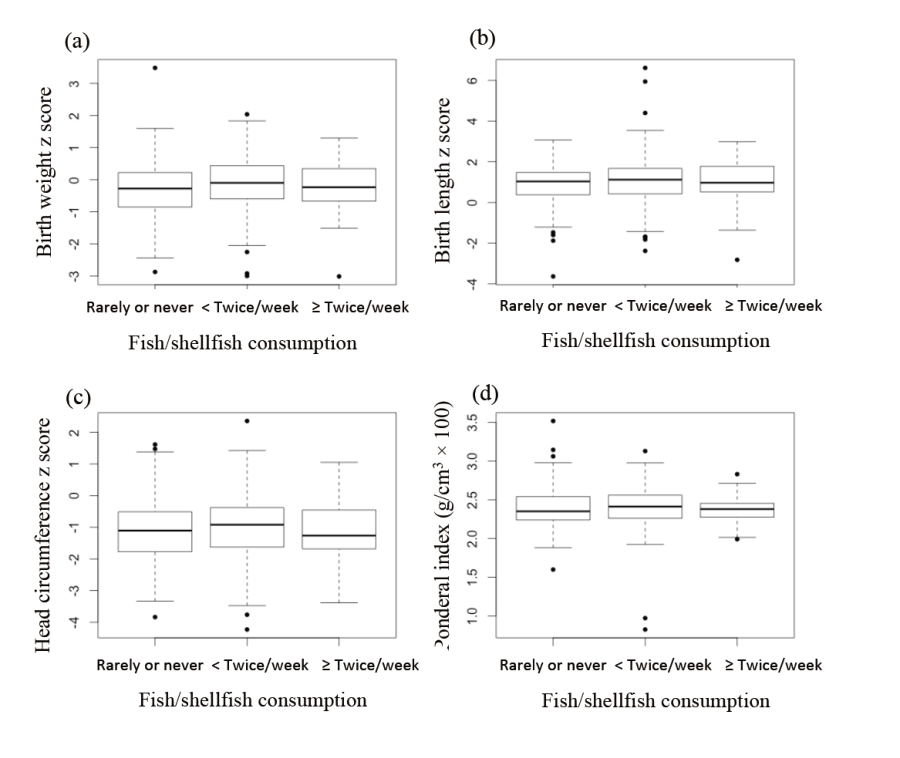
\includegraphics[scale=1]{Figures/Fig333.pdf}
  \caption[Bivariate analyses of fish/shellfish consumption versus birth outcomes (birth weight z score, birth length z score, head circumference z score, ponderal index)]{Bivariate analyses of fish/shellfish consumption versus birth outcomes (birth weight z score, birth length z score, head circumference z score, ponderal index). Oneway ANOVA test of fish/shellfish consumption versus (a) birth weight z score (p = 0.15), (b) birth length z score (p = 0.52), (c) head circumference z score (p = 0.48), and (d) ponderal index (p = 0.82) (n=398 for all).}
\end{figure}

\begin{figure}
  \centering
    \label{fig:Fig334}
  \includegraphics[scale=1]{Figures/Fig334.pdf}
  \caption[Bivariate analyses of serum selenium versus birth outcomes (birth weight z score, birth length z score, head circumference z score, ponderal index)]{Bivariate analyses of serum selenium (Se) versus birth outcomes (birth weight z score, birth length z score, head circumference z score, ponderal index). Spearman's correlation test of serum Se versus (a) birth weight z score (rho = -0.03, p = 0.60), (b) birth length z score (rho = 0.06, p = 0.28), (c) head circumference z score (rho = 0.04, p = 0.47), and (d) ponderal index (rho = -0.03, p = 0.59) (n=396 for all).}
\end{figure}

\begin{figure}
  \centering
    \label{fig:Fig335}
  \includegraphics[scale=1]{Figures/Fig335.pdf}
  \caption[Bivariate analyses of $\log_{10}$ serum selenium versus birth outcomes (birth weight z score, birth length z score, head circumference z score, ponderal index)]{Bivariate analyses of $\log_{10}$ serum selenium (Se) versus birth outcomes (birth weight z score, birth length z score, head circumference z score, ponderal index). Pearson's correlation test of $\log_{10}$ serum Se versus (a) birth weight z score (rho = -0.00001, p = 1.0), (b) birth length z score (rho = 0.02, p = 0.74), (c) head circumference z score (rho = 0.03, p = 0.50), and (d) ponderal index (rho = -0.0053, p = 0.92) (n=396 for all).}
\end{figure}



\chapter{Summary and Conclusions}

\section{Summary}

Hg is a toxic heavy metal and a global pollutant (National Research Council, 2000). MeHg is one of the most toxic forms of Hg, which biomagnifies along the food chain and accumulates in the human body (National Research Council, 2000). MeHg can cross the placenta and pass through the blood-brain barrier; the developing fetus is the most vulnerable population to the adverse effects of MeHg exposure (Clarkson \& Magos, 2006; Mergler et al., 2007). A few recent studies have shown that maternal exposure to low-level MeHg during pregnancy influenced fetal growth and development (reviewed in (Karagas et al., 2012)). For many people in the world, fish/shellfish is the primary source of MeHg exposure (National Research Council, 2000; Clarkson \& Magos, 2006), however, human dietary MeHg exposure also occurs through rice ingestion (Rothenberg et al., 2014). Rice does not contain the same beneficial nutrients for fetal development as fish/shellfish does, such as long chain polyunsaturated fatty acids, iodine, and selenium. Thus, maternal MeHg exposure mainly through rice ingestion may increase adverse influences on the developing fetus without the nutritional benefits from the consumption of fish/shellfish (Rothenberg et al., 2011). To our knowledge, few studies reporting rice Hg concentrations or rice ingestion and Hg biomarker levels were conducted in pregnant cohorts.

In Chapter 2, we measured the THg and/or MeHg concentrations in maternal scalp hair and whole blood in a cohort of newborns recruited at parturition from an inland rural area of Guangxi, China, where rice is a staple food and Hg contamination was considered minimal. The findings of this chapter confirmed the presence of low-level prenatal MeHg exposure occurring in this birth cohort, and indicated that maternal rice
ingestion during pregnancy contributed to the prenatal MeHg exposure, more so than the consumption of fish/shellfish. Meanwhile, the magnitude of prenatal MeHg in the Daxin cohort was comparable to other pregnant cohorts worldwide with low-level Hg exposure mainly through fish/shellfish consumption.

Furthermore, we examined the associations between socioeconomic characteristics and dietary MeHg intake. The study population of mothers represented a typical rural population of inland regions in Southern China. Similar to previous studies, we found that fish/shellfish consumption was higher for mothers who possessed a higher education level or had a higher household income (Knobeloch et al., 2005; Mahaffey et
al., 2009; Wang et al., 2009; Zhou et al., 2015; Hightower \& Brown, 2011). Notably, we found that mothers who were farmers consumed relatively low levels of fish/shellfish, which may be explained by the limited access to fish/shellfish. This is of interest because the food environment of famers is similar to the ``food desert''. Farmers in this cohort lived far away from the town of Daxin where diverse food (including fish/shellfish) was sold by local markets or groceries. Such a ``food desert'' may potentially affect farmers'
food access and nutritious status, however, fewer studies in China focused on this issue.

In Chapter 3, we examined the associations between maternal Hg biomarkers (i.e. hair THg, hair MeHg, and blood THg) and neonatal outcomes (i.e. birth weight, birth length, head circumference, and ponderal index) in both unadjusted and adjusted linear regression models. Firstly, we observed that birth weight z score was inversely associated with all Hg biomarkers in adjusted linear regression models, but the trends for hair THg
and hair MeHg were significant, while the trend for blood THg was borderline. Our findings were similar to some previous studies, which observed significantly inverse relationships between birth weight and some Hg biomarkers, such as cord blood THg (Ram�n et al., 2009; Lee et al., 2010) or maternal blood THg (Lee et al., 2010; Ou et al., 2015). Secondly, we observed inverse but non-significant adjusted linear relationships
between all Hg biomarkers and birth length z score or head circumference z score, which were consistent with other studies. For example, a few studies have reported that birth length was not related with prenatal Hg exposure in cord blood (Ding et al., 2013; Guo et al., 2013; Lederman et al., 2008; Wells et al., 2016), maternal hair (Drouillet-Pinard et al., 2010; Guo et al., 2013), or maternal blood (Lederman et al., 2008; Ding et al., 2013), in adjusted models. Also, six recent studies which evaluated head circumference (Ding et al.,
2013; Drouillet-Pinard et al., 2010; Gundacker et al., 2010; H. Guo et al., 2009; Lederman et al., 2008; Wells et al., 2016) observed non-significant associations between prenatal low-level MeHg exposure and head circumference in adjusted models. Lastly, the ponderal index was found to be significantly decreased with increasing blood THg in adjusted models, but not with other Hg biomarkers. Our findings were consistent with a Baltimore study, which observed an inverse association of cord blood MeHg and ponderal index after adjusting for potential covariates (Wells et al., 2016).

Moreover, this chapter provided an opportunity to investigate some protective factors related to fetal growth and development, such as fish/shellfish consumption and Se. However, the strength of the relationships between Hg biomarkers and birth outcomes in the Daxin cohort were not affected by the inclusion of fish/shellfish consumption frequency or maternal serum Se.

\section{Strengths and limitations}

A major strength of this study was the recruitment conducted in an area without Hg contamination, which is helpful to understand the general magnitude of MeHg exposure through rice consumption in a rice-eating population and the potential effects on fetal growth. Meanwhile, the sample size of this study is much larger than the previous studies (Maramba et al., 2006; Rothenberg et al., 2013), which improve the statistical power to evaluate the association between prenatal MeHg exposure and birth outcomes. Other strengths included the application of three maternal Hg biomarkers and four birth outcomes in this study, which made our findings more comprehensive and comparative.

There are several limitations in this study. The FFQ for the third trimester was conducted at parturition and was self-reported by the mothers, which might affect the validity of the maternal consumption information due to recall bias or wrong reporting. Moreover, we only measured 13 freshwater fish samples from Daxin local markets and did a literature review to obtain the Hg levels in other types of fish/shellfish. Future studies should measure Hg levels in all types of fish/shellfish included in the FFQ.

\section{Future studies}

Future studies of prenatal MeHg exposure through maternal consumption of rice and birth outcomes should be conducted to confirm these findings. For the present study, we collected the information of exposure and birth outcomes at parturition. Future studies about MeHg exposure during pregnancy could improve the study design. A longitudinal study conducted across the duration of pregnancy would be useful for determining the influence on fetal growth. For example, serial ultrasounds could be used to examine fetal
growth trajectory, and Hg levels in the maternal blood and hair could be measured at different stages during the pregnancy.

Additionally, the issue of ``food desert'' should be considered in future studies. The association between prenatal MeHg exposure and fetal growth may be affected by the maternal nutritional status due to the limited access to diverse or nutritious foods. To date, many studies have reported that the nutrition intake and diet quality before or during pregnancy is associated with fetal growth and development (Institute of Medicine (IOM), 1990; G. Wu, Bazer, Cudd, Meininger, \& Spencer, 2004). For instance, poor nutritious status before or during pregnancy was found to be associated with some adverse birth outcomes, such as small for gestational age (Mitchell et al., 2004) and lower birth weight (Sram, Binkova, Lnenickova, Solansky, \& Dejmek, 2005). Some recent studies reported that neighborhood food environments are associated with human dietary patterns (Walker, Keane, \& Burke, 2010). For example, a US study of adults observed that participants living far away from supermarkets (> 1 mile) were 25 - 46\% less likely to have a healthy dietary pattern than other respondents who did their food shopping within 1 mile of their home after adjustment for confounders (e.g. age, sex, race/ethnicity, and socioeconomic factors) (Moore \& Diez Roux, 2006). It is worth noting that the dietary quality and nutrition intake during pregnancy has a relationship with the food environment where the pregnant women live (Laraia, Siega-Riz, Kaufman, \& Jones, 2004). For example, in a North Carolina study, Laraia et al. observed that the distance to the closest supermarkets was positively associated with the diet quality index for pregnancy after adjusting for confounders (individual characteristics and other food retail outlets) (Laraia et al., 2004). However, to date, there are few studies on the food environment and fetal growth and the results are inconsistent. In a New York study, the authors observed that women living near a supermarket had significantly fewer low birth weight births after controlling for covariates, such as income (Lane et al., 2008). While in a Louisiana study, the authors reported that the local supermarket density was associated with neither the gestational age nor the birth weight-for-gestational age (Farley et al., 2006). Similarity, in a South Carolina study, authors found that either the accessibility or the availability of supermarkets and grocery stores was not associated with birth
outcomes and gestational age (Ma, Liu, Hardin, Zhao, \& Liese, 2015). Therefore, the food access in this study cohort may be a potentially important factor influencing the fetal growth, and should be evaluated in future studies about the association between prenatal MeHg exposure and birth outcome. For example, we can collect the information of individual access to nutritious or diverse foods (e.g. fish/shellfish), such as the distance from a participant's home to the nearest food market and the number of food markets within a 1-mile distance from participant's home. Then, we can evaluate the relationship of food access with MeHg exposure and birth outcomes.

\section{Conclusions}

In summary, these findings of this study confirm that prenatal exposure to MeHg was occurring among newborns born in Daxin County due to maternal consumption of rice during pregnancy. Despite the relatively low-level MeHg concentrations in maternal biomarkers (i.e. hair THg, hair MeHg, and blood THg), we observed significantly inverse linear relationships between birth weight and hair THg and hair MeHg, and also between ponderal index and blood THg in adjusted linear regression models. Future studies are needed to confirm these findings in other pregnant women cohorts who consume rice as a staple food. Given the human exposure to MeHg mainly through rice consumption in rice-eating populations, potential influences on fetal growth and development could have significant implications.
















%
%\usepackage[style=uscauthoryear]{biblatex}
\bibliography{biblio}


%\usepackage[style=uscauthoryear]{biblatex}
\bibliography{biblio}

\end{document}
%%%%%%%%%%%%%%%%%%%%%%%%%%%%%%%%%%%%%%%%%%%%%%%%%%%%%%%%%%%%%%%
